 
% example for dissertation.sty
\documentclass[
  % Replace oneside by twoside if you are printing your thesis on both sides
  % of the paper, leave as is for single sided prints or for viewing on screen.
  oneside,
  %twoside,
  11pt, a4paper,
  footinclude=true,
  headinclude=true,
  cleardoublepage=empty
]{scrbook}

\usepackage{dissertation}
\usepackage[utf8]{inputenc} %Needed for PT letters unavailable to EN language ( ç,....)
\usepackage{amsmath,mathtools,calc}
\usepackage{footnote}
\usepackage{hyperref}
\usepackage{multirow}
\usepackage[normalem]{ulem}


\usepackage{listings}
%LISTING - GENERAL
\lstset{
	basicstyle=\small,
	keywords={},
	numbers=left,
	numberstyle=\tiny,
	numbersep=5pt,
	breaklines=true,
	stepnumber=1,
    	frame=tB,
	%mathescape=true,
	escapeinside={(*@}{@*)}
}
%
%\lstset{ %
%	language=Java,							% choose the language of the code
%	basicstyle=\ttfamily\footnotesize,		% the size of the fonts that are used for the code
%	keywordstyle=\bfseries,					% set the keyword style
%	%numbers=left,							% where to put the line-numbers
%	numberstyle=\scriptsize,				% the size of the fonts that are used for the line-numbers
%	stepnumber=2,							% the step between two line-numbers. If it's 1 each line
%											% will be numbered
%	numbersep=5pt,							% how far the line-numbers are from the code
%	backgroundcolor=\color{white},			% choose the background color. You must add \usepackage{color}
%	showspaces=false,						% show spaces adding particular underscores
%	showstringspaces=false,					% underline spaces within strings
%	showtabs=false,							% show tabs within strings adding particular underscores
%	frame=none,								% adds a frame around the code
%	%abovecaptionskip=-.8em,
%	%belowcaptionskip=.7em,
%	tabsize=2,								% sets default tabsize to 2 spaces
%	captionpos=b,							% sets the caption-position to bottom
%	breaklines=true,						% sets automatic line breaking
%	breakatwhitespace=false,				% sets if automatic breaks should only happen at whitespace
%	title=\lstname,							% show the filename of files included with \lstinputlisting;
%											% also try caption instead of title
%	escapeinside={\%*}{*)},					% if you want to add a comment within your code
%	morekeywords={*,...}					% if you want to add more keywords to the set
%}

% ACRONYMS -----------------------------------------------------

%import the necessary package with some options
\usepackage[acronym,nonumberlist,nomain]{glossaries}

%enable the following to avoid links from the acronym usage to the list
%\glsdisablehyper

%displays the first use of an acronym in italic
\defglsdisplayfirst[\acronymtype]{\emph{#1#4}}


%the style of the Glossary
\glossarystyle{listgroup}

% set the name for the acronym entries page
\renewcommand{\glossaryname}{Acronyms}

%this shall be the last thing in the acronym configuration!!
\makeglossaries


% here are the acronym entries
\newacronym{mei}{MEI}{Mestrado em Engenharia Informática}
\newacronym{di}{DI}{Departamento de Informática}
\newacronym{um}{UM}{Universidade do Minho}

\newacronym{qos}{QoS}{Quality of Service}
\newacronym{soa}{SOA}{Service Oriented Architecture}

% these could go in an acronyms.tex file, and loaded with:
% \loadglsentries[\acronymtype]{Parts/Definitions/acronyms}
% when using this, you may want to remove 'nomain' from the package options

%% **MORE INFO** %%

%to add the acronyms list add the following where you want to print it:
%\printglossary[type=\acronymtype]
%\clearpage
%\thispagestyle{empty}

%to use an acronym:
%\gls{qps}

% compile the thesis in command line with the following command sequence:
% pdlatex dissertation.tex
% makeglossaries dissertation
% bibtex dissertation
% pdlatex dissertation.tex
% pdlatex dissertation.tex

% ----------------------------------------------------------------

% Title
\titleA{Implementing an Integrated Syntax}
\titleB{Directed Editor for LISS.} % (if any)
%\titleB{for LogoLISS with incremental compilation} % (if any)
%\subtitleA{First Part of Subtitle}
%\subtitleB{Second part of Subtitle} % (if any)

% Author
\author{Damien da Silva Vaz}

% Supervisor(s)
\supervisor{Professor Pedro Rangel Henriques}
\cosupervisor{Professor Daniela da Cruz}

% University (uncomment if you need to change default values)
% \def\school{Escola de Engenharia}
% \def\department{Departamento de Inform\'{a}tica}
% \def\university{Universidade do Minho}
% \def\masterdegree{Computer Science}

% Date
\date{\myear} % change to text if date is not today

% Keywords
%\keywords{master thesis}

% Glossaries & Acronyms
%\makeglossaries  %  either use this ...
%\makeindex	   % ... or this

% Define Acronyms
%%!TEX root = ../dissertation.tex

\newacronym{mei}{MEI}{Mestrado em Engenharia Inform\'{a}tica}
\newacronym{um}{UM}{Universidade do Minho}
%\glsaddall[types={\acronymtype}]



\ummetadata % add metadata to the document (author, publisher, ...)

\begin{document}
	% Cover page ---------------------------------------
	\umfrontcover	
	\umtitlepage
	
	% Add acknowledgements ----------------------------
	\chapter*{Acknowledgements}
	Firstly, I would like to thank my supervisor Pedro Rangel Henriques and co-supervisor Daniela da Cruz. They are the most who supported me throw this ambitious project and took me to the final stage of my university career.\newline
Thank you also to my family and friends (Ranim, Bruno, Chloé, Tiago, Tamara, Saozita, Nuno, David) for supporting me.\newline
And last but not least, I would like to dedicate this thesis to my, particularly, most beautiful mother.
Despite you couldn't be here to watch me conclude my studies. Wherever you are, I hope that you are proud of me.	
None of this could have been made without their unconditional help.

	% Add abstracts (en,pt) ---------------------------
	\chapter*{Abstract}
	The aim of this master work is to implement LISS language in ANTLR compiler generator system using an attribute grammar which create an abstract syntax tree (AST) and generate MIPS assembly code for MARS (MIPS Assembler and Runtime Simulator) .
Using that AST, it is possible to create a Syntax Directed Editor (SDE) in order to provide the typical help of a structured editor which controls the writing according to language syntax as defined by the underlying context free grammar.
	
	\cleardoublepage
	\chapter*{Resumo}
	O tema desta dissertação é implementar a linguagem LISS em ANTLR com um gramática de atributos e no qual, irá criar uma árvore sintática abstrata e gerar MIPS assembly código para MARS (MIPS Assembler and Runtime Simulator).
        Usando esta árvore sintática abstrata, criaremos uma SDE (Editor Dirigido a Sintaxe) no qual fornecerá toda a ajuda típica de um editor estruturado que controlará a escrita de acordo com a gramática.	
	
	% Summary Lists ------------------------------------
	\tableofcontents
	\listoffigures
	\listoftables
	%\lstlistoflistings
	%\listofabbreviations
	\printglossary[type=\acronymtype]
	\clearpage
	\thispagestyle{empty}

	
	\pagenumbering{arabic}
	
	% CHAPTER - Introduction -------------------------
	\chapter{Introduction}
In informatics, solving problems with computers is related to the necessity of helping the end-users, facilitating their life.
And all these necessities pass through developers who creates programs for this purpose.

However, developing programs is a difficult task; analyzing problems, and debugging software takes effort and time.

And this is why we must find a solution for these problems.

Developing a software package  requires tools to help the developers to maximize their programming productivity.
These tools are: on one hand, compilers to generate lower-level code (machine code) from the high-level source code (the input program written in an high-level programming language); on the other hand, editors to create that source code.
And to make easier and safer the programmers work, high-level programming languages were created for facilitating their work.

This is not enough to overcome all the difficulties for creating a program in a safety way and having  a high level productivity!

This is why we need to have fresh ideas and to implement more features to help on solving these problems.

\section{Objectives}
In this work, this project aims to develop an editor with the concept of a SDE (Syntax Directed Editor).

It is intended that the editor works with language designed by the members of the Language Processing group at UM which is called LISS.

LISS language will be specified by an attribute grammar that will be passed, as input, to ANTLR. The compiler generated by ANTLR will generate MIPS assembly code (lower-level source code).

The front-end and the back-end of that compiler will be explained and detailed along the next pages.

\section{Research Hypothesis}

\section{Thesis Outcomes}

\section{Document Structure}	

In this section, the project planned for this master thesis will be explained.

%Firstly, there is the necessity of generating the GIC from LISS language, like that we will see if there is no problem with the rules and definitions of a well grammar and follow the same grammar as LISS language (not being distinct) using ANTLR tool.

First, create an ANTLR version of the CFG grammar for LISS language.


Second, extend the LISS CFG to an AG in order to specify throw it the generation of MIPS assembly code.
To verify the correctness of the assembly code generated, a simple MIPS simulator, named MARS, will be selected to provide all the tools for checking it.

Third, the desired Structure-Editor, SDE, will be developed based on ANTLR.
It will be implemented in with Java SWING because ANTLR has always been implemented via Java and it is said, also, to use Java target as a reference implementation mirrored by other targets.
SWING is a GUI widget toolkit for Java which provides all the API for creating an interface with Java.
At this phase, we will create an IDE similar to other platforms but with the capacity of being a syntax-directed editor.

Fourthly, to complete the SDE functionality, an incremental compiler shall be included.
Incremental compilation ~\citep{RTD83a,Hol87a,VSK90a} means that only the part that was changed must be processed again. And like that, both tasks (edition and compilation) are done synchronously at the same time and having an editor which compiles cleverly.

Finally, exhaustive and relevant tests will be made with the tool created and, the outcomes will be analyzed and discussed.


%\chapter{State of the art}
\chapter{Languages and grammar: concept \& tools}
%       State of the art review; related work
A grammar ~\citep{Chomsky62a,Gau83a,WG84a,ASU86a,Kas91c,Muchnick97,Hopcroft2006b,Grune2012a} is a set of derivation rules (or production) that explains how words are used to build the sentences of a language.

A grammar ~\citep{DJB88a,Alb91a,Kas91a,SV91a,WAGA90,Rai80a,Fil83a,OPHCC2010} is considered to be a language generator and also a language recognizer (checking if a sentence is correctly derived from the grammar).

The rules describe how a string is formed using the language alphabet, defining the sentences that are valid according to the language syntax.

One of the most important researchers in this area was Noam Chomsky. He defined the notion of grammar in computer science's field.

He described that a formal grammar is composed by a finite set of production rules \\
\centerline{(left hand side $\mapsto$ right hand side)} \\
where each side is composed by a sequence of symbols.

These symbols are split into two sets : non terminals, terminals; the start symbol is a special non-terminal.

%And he explained that a grammar is composed by different symbols : non-terminals, terminals and start symbol.

%Non terminals are symbols which can be replaced, yet terminals are symbols which cannot be replaced.



There is, always, at least one rule for the start symbol (see Figure~\ref{fig:CFG}) followed by other rules to derive each non-terminal.
The non terminals are symbols which can be replaced and terminals are symbols which cannot be.

\begin{figure}[h!]
  \centering
    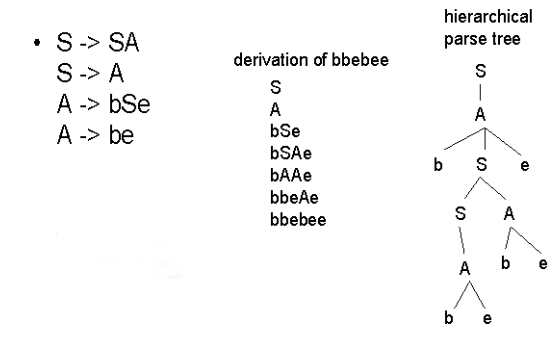
\includegraphics[width=0.7\textwidth]{img/GIC2.png}
    \caption{CFG example \protect\footnote{http://www.biiet.org/blog/wp-content/uploads/2013/07/img028.jpg}}
    \label{fig:CFG}
\end{figure}

%\footnote{http://www.biiet.org/blog/wp-content/uploads/2013/07/img028.jpg}
%falar dos terminais, nao terminais, start symbols e de Noam Chomsky

One valid sentences (Example in Figure ~\ref{fig:CFG}), could be : bbebee .

In the compilers area two major classes of grammars are used : CFG (Context-free grammar) and AG ( Attribute Grammar).

The difference between these two grammars are that a CFG is directed to define the syntax (only) and, AG contains semantic and syntax rules.

An AG is , basically, a GFC grammar extended with semantic definitions. It is a formal way to define attributes for the symbols that occur in each production of the underlying grammar. We can associate values to these attributes later, after processed with a parser; the evaluation will occur applying those semantic definition to any node of the abstract syntax tree.
These attributes are divided into two groups: synthesized attributes and inherited attributes.

The synthesized attributes are the result of the attribute evaluation rules for the root symbol of each subtree, and may also use the values of the inherited attributes. The inherited attributes are passed down from parent nodes to children or between siblings.

Like that it is possible to transport information anywhere in the abstract syntax tree which is one of the strength for using an AG (as seen on Listing ~\ref{lst:ag}).

%put an AG example !

\begin{comment}
\begin{figure}[h!]
  \centering
    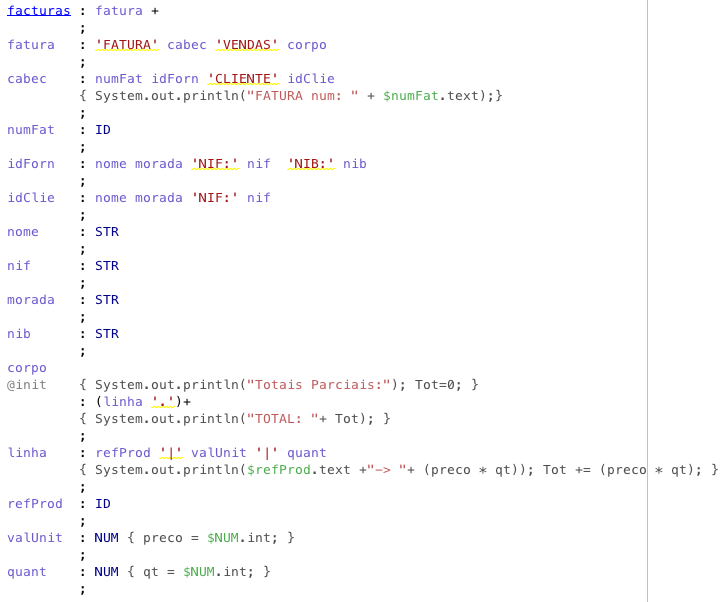
\includegraphics[width=0.9\textwidth]{img/ga.png}
    \caption{Example of an AG}
    \label{fig:GA}
\end{figure}
\end{comment}	

\begin{lstlisting}[caption={Example of an AG},label={lst:ag}]
facturas : fatura (facturas)*
         ;

fatura : 'FATURA' cabec 'VENDAS' corpo {System.out.println("Total Factura: "+$corpo.totOut);}
       ;

cabec : idFat idForn 'CLIENTE' idClie {System.out.println("Factura n: "+$idFat.text);}
      ;

idFat : numFat ;

numFat : ID ;

idForn : nome morada 'NIF:' nif 'NIB:' nib
       ;

idClie : nome morada 'NIF:' nif
       ;

nome :  STR ;

morada : STR;

nif : STR;

nib : STR;

corpo returns [int totOut]
    : linha '.' {$totOut += $linha.linhatot;}
      (linha '.' {$totOut += $linha.linhatot;})*
    ;

linha returns [int linhatot]
      : refProd '|' valUnit '|' quant {$linhatot = $valUnit.val * $quant.quan;System.out.println("Ref: "+$refProd.text+" Total linha: "+($linhatot)+" Euros");}
      ;
	
	refProd : ID;
valUnit returns [int val]
        : NUM {$val = $NUM.int;}
        ;
quant returns [int quan]
    : NUM {$quan = $NUM.int;}
    ;

\end{lstlisting}


In this way, an AG will be used to specify the translation from syntax tree directly into code for some specific machine or into another intermediate language.
For our thesis, the AG will be processed by ANTLR tool in order to build automatically the parser, the attribute evaluator, and the code generation.
%%%%%%%%%%%%%%%%%%%%%%%%%%%%%%%%%%%%%%%%%%%%%%%%%%%%%%

\section{Formal Grammar}
According to Noam Chomsky, a classic formalization of generative grammars is composed by:
\begin{itemize}
        \item A finite set N of nonterminals symbols.
        \item A finite set $\sum$  of terminals symbols.
        \item A finite set P of production rules.
        \item A start symbol S $\in$  P
\end{itemize}
A grammar is formally constructed by that tuple (N,$\sum$,P,S).



Grammar is a set of productions rules which describes the syntax of the language (not semantic). Each grammar has only one start symbol production that defines where the grammar begins.
%And there is two types after that the production rules are then applied in any order.
And each production is composed by two things : LHS (Left Hand Side) and RHS (Right and Side). Left Hand Side represents the non terminal and the right hand side represents the behaviour of the rule ( composed by non terminal and terminal).

\begin{lstlisting}[caption={A rule production},label={lst:ruleExample}]
     liss : 'program' identifier body
          ;
\end{lstlisting}

In ~\ref{lst:ruleExample}, we can see that it is composed by two sides. The left hand side and the right hand side, delimited by ':'.
On the LHS, 'liss' is a non-terminal and on the RHS, it is composed by the terminal 'program' followed by two non-terminals.
This is the syntax of one production rule of the grammar.

Now let's speak about the entire syntax of the LISS.

%\subsection{LISS Syntax}
\chapter{LISS language}

LISS ~\citep{CH07a} -that stands for Language of Integers, Sequences and Sets- is an imperative programming language, defined by the Language Processing members (Pedro Henriques and Leonor Barroca) at UM for teaching purposes (compiler course).

The idea behind the design of LISS language was to create a simplified version of the more usual imperative languages although combining functionalities from various languages.

It is designed to have atomic or structured integer values, as well as, control statements and block structure statements.

Now, let's explain in the next sections the basic statements of the language and its data types, using a context free gammar.

\section{LISS Data types}
\label{sec:data_types}

There are 5 types available.
From atomic to structured types, they are known as : integer, boolean, array, set and sequence.

Used for declaring a variable in a program, the data type gives us vital information for understanding what kind of value we are dealing with.

Let's obverse a LISS code example:

\begin{lstlisting}[caption={Declaring a variable in LISS},label={lst:declare_variable}]
  a -> integer;
  b -> boolean;
  c -> array size 5,4;
  d -> set;
  e -> sequence;
\end{lstlisting}

As we can see in Listing ~\ref{lst:declare_variable}, some variables ('a','b','c','d' and 'e')  are being declared each one associated to a type ('integer', 'boolean', 'array', 'set' and 'sequence').
Syntactically, in LISS, this is done by writing the variable name followed by an arrow and the type of the variable (see Listing ~\ref{lst:variable_declaration_BNF}).

\begin{lstlisting}[caption={CFG for declaring a variable in LISS},label={lst:variable_declaration_BNF}]
  variable_declaration : vars '->' type ';'
                     ;
  vars : var (',' var )*
     ;
  var : identifier value_var
    ;
  value_var :
          | '=' inic_var
          ;
  type : 'integer'
     | 'boolean'
     | 'set'
     | 'sequence'
     | 'array' 'size' dimension
     ;
  dimension : number (',' number )*
          ;
  inic_var : constant
         | array_definition
         | set_definition
         | sequence_definition
         ;
  constant : sign number
         | 'true'
         | 'false'
         ;
  sign :
     | '+'
     | '-'
     ;

\end{lstlisting}

Variables that are not initialized, have a default value (according to Table ~\ref{tbl:data_types}).

\begin{table}[]
\centering
\caption{LISS data types}
\label{tbl:data_types}
\begin{tabular}{|c|c|}
\hline
\textbf{Type}       & \multicolumn{1}{l|}{\textbf{Default Value}} \\ \hline
boolean             & false                                       \\ \hline
integer             & 0                                           \\ \hline
array               & {[}0,...,0{]}                               \\ \hline
set                 & \{\}                                        \\ \hline
sequence            & nil                                         \\ \hline
\end{tabular}
\end{table}

\newpage
Additionally, we may change the default values of the variables by initializing them with a different value (see an example in Listing ~\ref{lst:variable_declaration}).
This can be made by writing an equal symbol after the variable name and, then, inserting the right value according to the type (see example in Listing ~\ref{lst:variable_declaration_BNF}).

\begin{lstlisting}[caption={Initialize a variable},label={lst:variable_declaration}]
  a = 4, b -> integer;
  t = true -> boolean;
  vector1 = [1,2,3], vector2 -> array size 5;
  a = { x | x<10} -> set ;
  seq1 = <<10,20,30,40,50>>, seq3 = <<1,2>>, seq2 -> sequence;
\end{lstlisting}

Now, let's define which types are, correctly, associated with the arithmetic operators and functions in LISS (see Table ~\ref{tbl:type_operations}).


\begin{table}[]
\centering
\caption{Operations and signatures in LISS}
\label{tbl:type_operations}
\begin{tabular}{|c|c|}
\hline
\textbf{Operators \&\& Functions} & \multicolumn{1}{l|}{\textbf{Signatures}} \\ \hline
+ (add)                                   & integer x integer \verb+->+ integer                                        \\ \hline
- (subtract)                              & integer x integer \verb+->+ integer                                        \\ \hline
\verb+||+ (or)                            & boolean x boolean  \verb+->+ boolean                                       \\ \hline
++ (union)                                & set x set \verb+->+ set                                                    \\ \hline
/ (division)                              & integer x integer \verb+->+ integer                                        \\ \hline
* (multiply)                              & integer x integer \verb+->+ integer                                        \\ \hline
\&\& (and)                                & boolean x boolean \verb+->+ boolean                                        \\ \hline
** (intersection)                         & set x set \verb+->+ set                                                    \\ \hline
== (equal)                                & integer x integer \verb+->+ integer; boolean x boolean \verb+->+ boolean   \\ \hline
!= (not equal)                            & integer x integer \verb+->+ integer; boolean x boolean \verb+->+ boolean   \\ \hline
\textless  (less than)                    & integer x integer \verb+->+ boolean                                        \\ \hline
\textgreater  (greater than)              & integer x integer \verb+->+ boolean                                        \\ \hline
\textless= (less than or equal to)        & integer x integer \verb+->+ boolean                                        \\ \hline
\textgreater= (great than or equal to)    & integer x integer \verb+->+ boolean                                        \\ \hline
in (contains)                              & integer x set \verb+->+ boolean                                            \\ \hline
tail                                      & sequence \verb+->+ sequence                                                \\ \hline
head                                      & sequence \verb+->+ integer                                                 \\ \hline
cons                                      & integer x sequence \verb+->+ sequence                                      \\ \hline
delete                                    & integer x sequence \verb+->+ sequence                                      \\ \hline
copy                                      & sequence x sequence \verb+->+ void                                         \\ \hline
cat                                       & sequence x sequence \verb+->+ void                                         \\ \hline
isEmpty                                   & sequence \verb+->+ boolean                                                 \\ \hline
length                                    & sequence \verb+->+ integer                                                 \\ \hline
isMember                                  & integer x sequence \verb+->+ boolean                                       \\ \hline
\end{tabular}
\end{table}

\newpage

So, in Table ~\ref{tbl:type_operations}, we list the operators and functions, available in LISS, and their signature.
In order to understand the table better, we will explain how to read the table and its signature with one example.

Consider the symbol '+' (Table ~\ref{tbl:type_operations}), indicates that both operands must be of type integer.
The result of that operation, indicated by the symbol '\verb+->+', will be an integer.
%Notice that semantically, operations must be validated according to the table ~\ref{tbl:type_operations}, otherwise the operations would be incorrect and throw an error.
Semantically, operations must be valid according to Table ~\ref{tbl:type_operations}; otherwise the operations would be incorrect and throw an error.

\bigbreak

\textbf{Arrays.}
LISS supports a way of indexing a collection of integer values such that each value is uniquely addressed. LISS also supports an important property of multidimensionality.

Called as 'array', it is considered to be a static structured type due to the fact that its dimensions and maximum size of elements in each dimension is fixed at the declaration time.

%One of its, most important, property is that he may have multiple dimension.

The operations defined over arrays are:

\begin{enumerate}
\item \textit{indexing} %- denoted by '[' and ']', it selects the value of the chosen indexed array.
\item \textit{assignment} %- 
\end{enumerate}

%explaining probably indexing and assignment

Arrays can be initialized, in the declaration section, partially or completely in each dimension.
For example, consider an array of dimension 3x2 declared in the following way:

\begin{lstlisting}
  array1 = [[1,2],[5]] -> array size 3,2;
\end{lstlisting} 

Thi is equivalent to the initialization below:

\begin{lstlisting}
  array1 = [[1,2],[5,0],[0,0]] -> array size 3,2;
\end{lstlisting}

Notice that the elements that are not explicitly assigned, are initialized with the value 0 (see Table ~\ref{tbl:data_types}).

The grammar for array declaration and initialization is shown below.

\begin{lstlisting}
  array_definition : '[' array_initialization ']'
                 ;

  array_initialization : elem (',' elem)*
                     ;

  elem : number
     | array_definition
     ;
\end{lstlisting}

\bigbreak

\textbf{Sets.}
The type \textit{set}, in LISS, is a collection of integers with no repeated numbers.

It is defined by an expression, in a comprehension, instead of by enumeration of its element.
A \textit{set} variable can have an empty value and, syntactically, this is done by writing '\verb+{}+'.

To define a set by comprehension, the free variable and the expression shall be return between curly brackets. The 'identifier' (free variable) is separated from the expression by an explicit symbol '\verb+|+'. 

The expression is built up from relational and boolean operators to define an integer interval.

The operations defined for sets are :
\begin{enumerate}
\item \textit{union}
\item \textit{intersection}
\item \textit{in} (membership)
\end{enumerate}


Let's see an example of its syntax below:

\begin{lstlisting}
  set1 = {x | x < 6 && x > -7} -> set;
\end{lstlisting}

This declaration defines a set including all the integers from -7 to 6 (open interval) and others numbers are not included in the set.

The syntax for set declaration and initialization is :

\begin{lstlisting}
  set_definition : '{' set_initialization '}'
               ;

  set_initialization :
                   | identifier '|' expression
                   ;
\end{lstlisting}

\bigbreak

\textbf{Sequences.}
Considered as a dynamic array of one dimension, the type sequence is a list of ordered integers. But, in opposition to the concept of an array, its size is not fixed; this means that it grows dinamicallly at run time like a linked list.
A sequence can have the empty value (syntactically done by writing '\verb+<<>>+').
If not empty, the sequence value is defined by enumerating its components (integers) in the right order.
Let's see deeper with one example:

\begin{lstlisting}[caption={Example of valid operations using sequence on LISS},label={lst:sequence_example_use}]
  c=<<1,2,3>> -> sequence;
\end{lstlisting}

In the example of Listing ~\ref{lst:sequence_example_use} the sequence is defined by three numbers (3,2,1). 

The operations defined for the sequence are:
\begin{enumerate}
\item \textit{tail} (all the elements but the first)
\item \textit{head} (the first element of the sequence)
\item \textit{cons} (adds an element in the head of the sequence)
\item \textit{delete} (remove a given element from the sequence)
\item \textit{copy} (copies all the elements to another sequence)
\item \textit{cat} (concatenates the second sequence at the end of the first sequence)
\item \textit{isEmpty} (true if the sequence is empty)
\item \textit{length} (number of elements of the sequence)
\item \textit{isMember} (true if the number is an element of the sequence)
\end{enumerate}
Those operations will be explained further and deeper.

The grammar below defines how to declare a sequence:

\begin{lstlisting}
  sequence_definition : '<<' sequence_initialization '>>'
                    ;

  sequence_initialization :
                        | values
                        ;

  values : number (',' number )*
       ;

\end{lstlisting}

\subsection{LISS lexical conventions}

Once you've declared a variable of a certain type, you cannot redeclare it again with the same name.

The variable name must be unique (see Listing ~\ref{lst:variable_name_single}).

\begin{lstlisting}[caption={Conflicts with variable names},label={lst:variable_name_single}]
  program single_variable_name{
    declarations
      int=1 -> integer;
      int=true -> boolean; //cannot declare this variable with this name (already exists)
    statements
  }
\end{lstlisting}

Keywords cannot be used as variable names.

For example, you cannot declare a variable with the name \textit{array} due to the fact that \textit{array} is a keyword in LISS (in this case, a type).

See the example in Listing ~\ref{lst:keyword_reserved_name}.
\begin{lstlisting}[caption={Conflicts with keyword names},label={lst:keyword_reserved_name}]
  array -> array size 3,4; //variable 'array' cannot be declared as a name
  integer -> integer;
\end{lstlisting}

Variable names contain only letters and numbers, or the underscore sign. However the first character of the variable name must be a letter (lower or upper case).
See the example below:

\begin{lstlisting}[caption={},label={}]
  My_variable_1
  MyVariable1
\end{lstlisting}

Numbers are composed of digits (one or more). 
Nothing more is allowed.

See example below:

\begin{lstlisting}[caption={},label={}]
  1562
  1
\end{lstlisting}

A string is a sequence of n-characters enclosed by double quotes.

See example below:

\begin{lstlisting}[caption={},label={}]
  "This is a string"
\end{lstlisting}

\section{LISS blocks and statements}

A LISS program is always composed of two parts: declarations and statements (a program block).
LISS language is structured with a simple hierarchy.
And this is done by structuring LISS code as a block.

Any program begins with a name then appear the declaration of variables and subprograms. After that appear the flow of the program by writing statements.

Let's see one example (see Listing ~\ref{lst:block_liss}).

\begin{lstlisting}[caption={The structure of a LISS program (example)},label={lst:block_liss}]
  program sum{
    declarations
        int=2 -> integer;
    statements
        writeln(int+3);
  }
\end{lstlisting}

So a program in LISS begins by, syntactically, writing 'program' and then the name of the program (in this case, the name is 'sum').
A pair of curly braces delimits the contents of the program; that is done by opening it after the name of the program and closing it at the end of the program.
After the left brace, appear the declaration and statement blocks.

As in a traditional imperative language (let's compare 'C language'), if we don't take the habit of declaring the variable always in a certain part of the code, it becomes confusing. This makes the programmer's life harder to understand the code when the code is quite long.

So, in LISS, we always declare variables first (syntactically written by 'declarations')  and then the statements (syntactically written by 'statements').
This is due to the fact that LISS wants to help the user to create solid and correct code. And in this case, the user will always know that all the variable declarations will be always at the top of the statements and not randomly everywhere (see grammar in Listing ~\ref{lst:program_grammar}).

\begin{lstlisting}[caption={CFG for program in LISS},label={lst:program_grammar}]
  liss : 'program' identifier body
     ;

  body : '{'
       'declarations' declarations
       'statements'   statements
       '}'
     ;
\end{lstlisting}

\subsection{LISS declarations} \label{subsec:liss_declarations}
The declaration part is divided into two other parts: variable declarations and subprogram declarations, both optional.

The first part is explained in section ~\ref{sec:data_types}; the subprogram part will be discussed later in section ~\ref{sec:subprograms}.

This part is specified by the following grammar (see Listing ~\ref{lst:declarations_grammar}).

\begin{lstlisting}[caption={CFG for declarations in LISS},label={lst:declarations_grammar}]
  declarations : variable_declaration* subprogram_definition*
             ;
\end{lstlisting}

\subsection{LISS statements}

As said previously, under the statements part, we control and implement the flow of a LISS program.
In LISS, we may write none or, one or more statements consecutively.

Every statement ends with a semicolon, unless two type of statements (conditional and cyclic statements) as shown in Listing ~\ref{lst:liss_statements_bnf}.

\begin{lstlisting}[caption={CFG for statements in LISS},label={lst:liss_statements_bnf}]
  statements : statement*
           ;
  statement : assignment ';'
          | write_statement ';'
          | read_statement ';'
          | function_call ';'
          | conditional_statement
          | iterative_statement
          | succ_or_pred ';'
          | copy_statement ';'
          | cat_statement ';'
          ;
\end{lstlisting}

Let's see one example of a LISS program which shows how the language shall be used (see Listing ~\ref{lst:statements_example}).

\begin{lstlisting}[caption={Example of using statements in LISS},label={lst:statements_example}]
  program factorial{
    declarations
        res=1, i -> integer;
    statements
        read(i);
        for(j in 1..i){
            res=res*j;
        }
        writeln(res);
  }
\end{lstlisting}

\textbf{Assignment.} This statement assigns, as it is called, values to a variable and it is defined for every type available on LISS.
This operation is done by writing the symbol "=" in which a variable is assigned to the left side of the symbol and a value to the right side of the symbol.

Notice that an assignment requires that the variable on the left and the expression on the right must agree in type.

Let's see in Listing ~\ref{lst:assignment_example} an example.

\begin{lstlisting}[caption={Example of assignment in LISS},label={lst:assignment_example}]
  program assignment1{
    declarations
      intA -> integer;
      bool -> boolean;  
    statements
      intA = -3 + 5 * 9;
      bool = 2 < 8;
  }
\end{lstlisting}

In Listing ~\ref{lst:assignment_example}, we can see assignment statements of integers and boolean types.
Those assignments are correct, as noticed in the previous paragraphs, because they have the same type on the left and right side of the symbol equals (operations of integers assigned to a variable of integer type and operation of booleans assigned to a variable of boolean type).

The grammar that rules the assignment is shown at Listing ~\ref{lst:assignment_bnf}.

\begin{lstlisting}[caption={CFG for assignment in LISS},label={lst:assignment_bnf}]
  assignment : designator '=' expression
           ;
\end{lstlisting}

\textbf{I/O.} The input and output statements are also available in LISS.

The \textit{read} operations, called syntactically as 'input' in LISS, assign a value to a variable obtained from the standard input and require to be an atomic value (in this case, only an integer value).


\begin{lstlisting}[caption={Example of input operation in LISS}, label={lst:input_example}]
  program input1{
    declarations
      myInteger -> integer;
    statements
      input(myInteger);
  }
\end{lstlisting}

Notice that, in Listing ~\ref{lst:input_example}, the variable \textit{myInteger} must be declared  and must be integer otherwise the operations fails.
The grammar that rules the input statement, is shown in Listing ~\ref{lst:input_bnf}.

\begin{lstlisting}[caption={CFG for input operation in LISS}, label={lst:input_bnf}]
 read_statement : 'input' '(' identifier ')'
               ; 
\end{lstlisting}

The \textit{write} operations, called syntactically as 'write' or 'writeln' in LISS, print an integer value in the standard output.
Notice that 'write' operation only prints the value and doesn't move to a new line; instead, 'writeln' moves to a new line at the end.

Listing ~\ref{lst:output_example} shows some more examples.

\begin{lstlisting}[caption={Example of output operations in LISS},label={lst:output_example}]
  writeln(4*3);
  writeln(2);
  writeln();
\end{lstlisting}

Note that the write statement may have as assignment, an atomic value as well as an empty value or some complex arithmetic expression (see grammar in ~\ref{lst:output_bnf}).

\begin{lstlisting}[caption={CFG for output operation in LISS},label={lst:output_bnf}]
  write_statement : write_expr '(' print_what ')'
                ;

  write_expr : 'write'
           | 'writeln'
           ;

  print_what :
           | expression
           ;
\end{lstlisting}

\textbf{Function call.} The function call is a statement that is available for using the functions created in the program under the section 'declarations' (as described in Section ~\ref{subsec:liss_declarations}).
This will allow reusing functions that were created by calling them instead of creating duplicated code.

See Listing ~\ref{lst:call_function_example} for a complete example.

\begin{lstlisting}[caption={Example of call function in LISS},label={lst:call_function_example}]
 program SubPrg {

  declarations

    a = 4, b= 5, c= 5 -> integer;
    d = [10,20,30,40], ev -> array size 4;


    subprogram calculate() -> integer
    {
      declarations
            fac = 6 -> integer;
            res = -16 -> integer;

        subprogram factorial(n -> integer; m -> array size 4) -> integer
            {
              declarations
                    res = 1 -> integer;
              statements
                    while (n > 0)
                    {
                        res = res * n;
                        n = n -1;
                    }

                    for (a in 0..3) stepUp 1
                    {
                      d[a] = a*res;
                    }
                    return res;
            }
      statements
            res = factorial(fac,d);
            return res/2;
    }


  statements

    a = calculate();
    writeln(a);
    writeln(d);
}
\end{lstlisting}

In Listing ~\ref{lst:call_function_example}, we can see that the function \textit{calculate()}, called in the main program, and that is created under the declarations section.

The grammar who rules the function call is shown in Listing ~\ref{lst:call_function_bnf}.

\begin{lstlisting}[caption={CFG for call function in LISS},label={lst:call_function_bnf}]
  function_call : identifier '(' sub_prg_args ')'
              ;
  sub_prg_args :
             | args
             ;
  args : expression (',' expression )*
     ;

\end{lstlisting}

\subsection{LISS control statements}

LISS language includes some statements for controlling the execution flow at runtime with two different kind of behaviour.

The first one is called conditional statement and it has only one variant in LISS language (see Listing ~\ref{lst:control_statements}).

The second one is called cyclic statement or iterative statement, and it has two variants (see Listing ~\ref{lst:control_statements}).

\begin{lstlisting}[caption={CFG for control statement in LISS},label={lst:control_statements}]
  conditional_statement : if_then_else_stat
                      ;
  iterative_statement : for_stat
                    | while_stat
                    ;
\end{lstlisting}

These control statements, mimics the syntax and the behaviour  of other modern imperative language.

\paragraph{Conditional}

The if-statement, which is common across many modern programming languages, performs different actions according to decision depending on the truth value of a control conditional expression: an alternative 'else' block is also allowed (optional).

If the conditional expression evaluates 'true', the content of 'then' block will be executed. Otherwise, if the condition is 'false', the 'then' block is ignored; and if an 'else' block is provided it will be executed alternatively.

Let's see an example in Listing ~\ref{lst:if_program}.

\begin{lstlisting}[caption={LISS syntax of a if statement},label={lst:if_program}]
  if(y==x)
  then{
    x=x+1;
  }else{
    x=x+2;
  }
\end{lstlisting}

The code shown in Listing ~\ref{lst:if_program}, means that the if-statement evaluates the conditional expression 'y==x'.
If the expression, which must be boolean, is true, then every action in the 'then' block will be executed and the block 'else' will be ignored.
Otherwise, if the condition is false, every action in the 'else' block is executed ignoring the 'then' block.

If the else-statement is not provided, the if-statement will finish and do not perform any actions.


The syntax of the if-statement in LISS is shown in Listing ~\ref{lst:if_bnf}.



\begin{lstlisting}[caption={CFG for iterative statement in LISS},label={lst:if_bnf}]
  if_then_else_stat : 'if' '(' expression ')'
                    'then' '{' statements '}'
                    else_expression
                    ;

  else_expression :
                | 'else' '{' statements '}'
                ;
\end{lstlisting}

\paragraph{Iterative}

We should take a look at the behaviour of each iterative control statement to understand it deeper.

The  for-statement offers two variants to control the repetition.
Normally, in a conventional way, the for-loop has a control variable which takes a value in a given range and step up or step down by a default or an explicit value.

In LISS, the control variable is set in a given integer interval defined by the lower and upper bounds. By default, the step is one, which means that the control variable is incremented by one at the end of each iteration but it is possible to increment or decrement it by a different value, setting it explicitly.
Additionally, we may write a condition for filtering the values in the interval.
This can be done as shown in the following example:
\begin{lstlisting}[caption={LISS syntax of a for-loop statement},label={lst:for-loop}]
  for(a in 1..10) stepUp 2 satisfying elems[a]==1{
	  ...
  }
\end{lstlisting}
In Listing ~\ref{lst:for-loop}, the control variable 'a' is set to a range 1 to 10 and would be increased (due to the 'stepUp' constructor) by 2. Also there is a filter condition (after the 'satisfying' keyword) that restricts the values of 'a' to those that makes the condition 'elems[a]==1' true. Notice that the filter expression must be boolean. 

After each cycle, the control variable will be incremented with value 2 and the filter condition tested again. 

This is the first way of expressing the control in a for-loop statement. Let's see the second way in the sequel.

There is also the possibility to assign to the control variable the values in an array, like illustrated in the following example:

\begin{lstlisting}[caption={LISS syntax of a for-each statement on array},label={lst:for-each_array}]
  for(b inArray elems){
       	...
  }
\end{lstlisting}
In Listing ~\ref{lst:for-each_array}, the control variable  'b' is assigned with all of the elements of the array and begins with his lower index (zero) until his upper index (size of the array minus one).
Notice that, in this case, we cannot apply an increment or decrement neither a filter condition.

The next grammar fragment describes the cycle 'for' in LISS:

\begin{lstlisting}[caption={CFG for for-statement in LISS}]
  for_stat : 'for' '(' interval ')' step satisfy
           '{' statements '}'
         ;
  interval : identifier type_interval
         ;
  type_interval : 'in' range
              | 'inArray' identifier
              ;
  range : minimum '..' maximum
      ;
  minimum : number
        | identifier
        ;
  maximum : number
        | identifier
        ;
  step :
     | up_down number
     ;
  up_down : 'stepUp'
        | 'stepDown'
        ;
  satisfy :
        | 'satisfying' expression
        ;
\end{lstlisting}

%write the for statetement with step and satisfy explication

Finally, the while-statement consists in a block of code that is executed repeatly until the control condition evaluates 'false'. 

Each time that the 'while' block is performed, the conditional expression associated will be evaluated again to decide whether to repeat the execution of the statements in the block or to continue the normal program flow.

Let's see an example in Listing ~\ref{lst:while_program}.

\begin{lstlisting}[caption={LISS syntax of a while-statement in LISS},label={lst:while_program}]
  while (n > 0)
  {
    res = res * n;
    pred n;
  }
\end{lstlisting}

In Listing ~\ref{lst:while_program}, the while-statement is controled by the conditional expression '\verb+n>0+' that is evaluated at the beginning. If the condition is true, then all the actions that are inside the braces will be performed. Later, after executing all the actions, the condition will be evaluated again. If the condition remains 'true', then those actions would be executed again otherwise if the condition is false, the while-statement will be exited.

The syntax that rule the while-statement is shown below:

\begin{lstlisting}[caption={CFG for while-statement in LISS}]
  while_stat : 'while' '(' expression ')'
             '{' statements '}'
             ;
\end{lstlisting}



\subsection{Others statements}

LISS language offers other statements to make it more expressive easing the codification of any imperative algorithm.

\textbf{Succ/Pred.} Those statements are available for incrementing or decrementing a variable. This is a common situation in modern programming languages, making life easier for the developers. 

The keyword 'succ' means increment (successor) and the syntax 'pred' means decrease (predecessor). Only integer variables can be used with those constructors.

Listing ~\ref{lst:succ_or_pred_example} illustrates both statements.

\begin{lstlisting}[caption={Example of using succ/pred in LISS}, label={lst:succ_or_pred_example}]
  succ int1;
  pred int1;
\end{lstlisting}

As we can see in Listing ~\ref{lst:succ_or_pred_example}, variable 'int1' is, first, incremented by 1 and then it is decremented also by 1.

Grammar of 'succ' and 'pred' in LISS is shown in Listing ~\ref{lst:succ_or_pred_bnf}.


\begin{lstlisting}[caption={CFG for succ and pred in LISS}, label={lst:succ_or_pred_bnf}]
  succ_or_pred : succ_pred identifier
             ;
  succ_pred : 'succ'
          | 'pred'
          ;
\end{lstlisting}

\textbf{Copy statement.}
This statement is applied only to variables of type sequence.
Basically, it copies one sequence to another sequence.
Let's see an example in Listing ~\ref{lst:copy_example}.

\begin{lstlisting}[caption={Example of copy statement in LISS},label={lst:copy_example}]
  copy(seq1,seq2);
\end{lstlisting}

Notice that 'copy' is a statement and not a function: it modifies the arguments but does not return any value.

In Listing ~\ref{lst:copy_example}, the statement 'copy' copies the content of the variable \textit{seq1} to \textit{seq2}.

The grammar for 'copy' statement is in Listing ~\ref{lst:copy_bnf}.

\begin{lstlisting}[caption={CFG for copy statement in LISS},label={lst:copy_bnf}]
  copy_statement : 'copy' '(' identifier ',' identifier ')'
                 ;
\end{lstlisting}

\textbf{Cat statement.}

'Cat' statement is simular to 'copy', it only operates with variables of type sequence.
The behaviour of this statement is to concatenate a sequence to another sequence.
Let's see an example in Listing ~\ref{lst:cat_example}).

\begin{lstlisting}[caption={Example of cat statement in LISS},label={lst:cat_example}]
  cat(seq1,seq2);
\end{lstlisting}

In Listing ~\ref{lst:cat_example}, 'cat' concatenates the content of \textit{seq2} to \textit{seq1}.
Again, 'cat' is not a function; it modifies the arguments instead of returning a value.

The grammar for cat-statement is shown in Listing ~\ref{lst:cat_bnf}.

\begin{lstlisting}[caption={CFG for cat statement in LISS},label={lst:cat_bnf}]
  cat_statement : 'cat' '(' identifier ',' identifier ')'
                ;
\end{lstlisting}

\section{LISS subprograms}
\label{sec:subprograms}

In LISS, it is possible to organize the code by splitting the general block of statements into sub-programs. This allows the programmer to reuse or to give more clarity to his code by creating functions or procedures.
Also, it is possible to create sub-programs inside sub-programs by using a nesting strategy.

The syntax that defines a sub-program in LISS is shown in Listing ~\ref{lst:block_structure}.

\begin{lstlisting}[caption={CFG for block structure in LISS},label={lst:block_structure}]
  subprogram_definition: 'subprogram' identifier '(' formal_args ')' return_type f_body
                     ;
  f_body : '{'
         'declarations' declarations
         'statements' statements
         returnSubPrg
         '}'
       ;
  formal_args :
            | f_args
            ;
  f_args  : formal_arg (',' formal_arg )*
        ;
  formal_arg : identifier '->' type
           ;
  return_type :
            | '->' typeReturnSubProgram
            ;
  returnSubPrg :
             | 'return' expression ';'
             ;
\end{lstlisting}

Note that every variable declared inside of a sub-program is local, and it can be accessed only by other nested sub-programs.
However, variables declared in the program (not in a sub-program) are considered global and can be accessed by any sub-program. The usual scope rules are applied to LISS.

As can be inferred from the syntax above (Listing ~\ref{lst:block_structure}), the body of a sub-program is identical to the body of a program --- the same declarations can be made and similar statements can be used.










%Also, in LISS language, variables are declared firstly and then we may code the program.
%Notice that this restriction is done for a better experience of the programmer. 
%This means that variables must be declared always on top of the program before they will be used on the rest of the program.


%It allows handling integers, sets of integers, dynamic sequences, complex numbers, polynomials, etc., etc~\citep{CH07d,CH07a,CH06a,CH06b,CH05a}.


\newpage


%write appendix , code gic liss

\section{Evolution of LISS syntax}
Due to the maturity of the language already done along the years, we have added some few but extra changes for a better experience of the programming language.
%The syntax of the LISS language (Figure ~\ref{lst:GIC_LISS} ), has been constructed with ANTLR which is ANother Tool for Language Recognition where it collaborates with the Java platform.

%One of the first objectives is that we have changed the format of the syntax. We have translated the old LISS language to a brand new extended BNF format (as shown in Figure ~\ref{lst:GIC_LISS}).

One of the first changes was concerned with declarations in order to avoid mixing functions and variable declarations.
We, indirectly, teach the programmer by doing it in the right way. So we declare, first, the variables and then the functions.
\begin{lstlisting}[caption={},label={lst:declaration_LISS}]
declaration : variable_declaration * subprogram_definition *
            ;
\end{lstlisting}

Another change was to add punctuation after each statement (see Figure ~\ref{lst:statement_LISS}).
\begin{lstlisting}[caption={Function statement},label={lst:statement_LISS}]
statement : assignment  ';'
          | write_statement  ';'
          | read_statement  ';'
          | conditional_statement
          | iterative_statement
          | function_call ';'
          | succ_or_pred  ';'
          | copy_statement  ';'
          | cat_statement  ';'
          ;
\end{lstlisting}

Another change was adding also a 'cat\_statement' rule which works with only sequences. It concatenates a sequence with another sequence.

Regarding arrays, it was previously possible to use any expression to access elements of the array. So it was possible to index with a boolean expression what does not make any sense.
Now only integers are allowed (see in Listing ~\ref{lst:elem_array_LISS}).


\begin{lstlisting}[caption={Rule element of array},label={lst:elem_array_LISS}]
elem_array : single_expression (',' s2=single_expression )*
           ;
\end{lstlisting}

In the previous version of LISS, it was allowed to create a boolean expression associating relational operators, but we decided to change that and not permit associativity; only able to create one boolean expression (see Listing ~\ref{lst:expression_LISS}).
It does not make sense to have an expression like that : '3 == 4 == 5 != 6'.
\begin{lstlisting}[caption={Rule for Boolean expression},label={lst:expression_LISS}]
expression : single_expression (rel_op single_expression )?
           ;
\end{lstlisting}

We added the possibility of using parenthesis on expressions (see Listing ~\ref{lst:factor_LISS}).

\begin{lstlisting}[caption={Rule factor},label={lst:factor_LISS}]
factor: '(' expression ')'
      ;
\end{lstlisting}

We changed the rules of two pre-defined functions: 'cons' and 'del'. These functions were working both in the same way. Waiting for an expression and a variable as arguments. Now, we decide to change that allowing to expression as arguments giving more expressive power to those functions (see Listing ~\ref{lst:cons_del_LISS}).

\begin{lstlisting}[caption={Rule cons and delete},label={lst:cons_del_LISS}]
cons // integer x sequence -> sequence
     : 'cons' '(' expression ',' expression ')'
     ;

delete // del : integer x sequence -> sequence
       : 'del' '(' expression ',' expression ')'
       ;
\end{lstlisting}

Besides adding some improvements to the grammar, we additionally deleted a rule which we thought not necessary to control the for-statement (see Listing ~\ref{lst:type_interval_LISS}).
\begin{lstlisting}[caption={Rule type interval},label={lst:type_interval_LISS}]
type_interval : 'in' range
              | 'inArray' identifier
              //| 'inFunction' identifier
              ;
\end{lstlisting}

Last but not least, we also added comments to the programming language, giving more power to the programmer.

\begin{lstlisting}[caption={Lexical rule for Comment},label={lst:comments_LISS}]
fragment
COMMENT
    : '/*'.*?'*/' /* multiple lines comment*/
    | '//'~('\r' | '\n')* /* single line comment*/
    ;
\end{lstlisting}











\chapter{Target machine: MIPS}

%\section{MIPS}

MIPS, from Microprocessor without Interlocked Pipeline Stages, is a Reduced Instruction Set Computer (RISC) developed by MIPS Technologies. 
Born in 1981, a team led by John L. Hennessy at Stanford University began to work on the first MIPS processor.

The main objective for creating MIPS, was to increase performance with deep pipelines, a main problem back to the 80's. 
Some instructions, as division, take a longer time to complete; if the CPU needs to wait that the division ends before passing to the next instruction into the pipeline, the total time is greater. If it can be done without that waiting time, the total process will be faster.

As MIPS solved those problems, it was primarly used for embedded systems and video games consoles (which requires a lot of arithmetic computation). 
% until late 2006, when it came to computers.

Now, the architecture of MIPS, along the years, has gained maturity and provides different versions of it (MIPS32, MIPS64....) \footnote{according to \url{https://imgtec.com/mips/architectures} (See also wikipedia \url{https://en.wikipedia.org/wiki/MIPS_instruction_set})}.

Figure ~\ref{fig:MIPSarchitecture} \footnote{ from \url{https://upload.wikimedia.org/wikipedia/commons/thumb/e/ea/MIPS_Architecture_(Pipelined).svg/300px-MIPS_Architecture_(Pipelined).svg.png}}  illustrate the architecture of MIPS.

%The architecture of MIPS is composed by 5 stages (see Figure ~\ref{fig:MIPSarchitecture}).

\begin{figure}[h!]
  \centering
    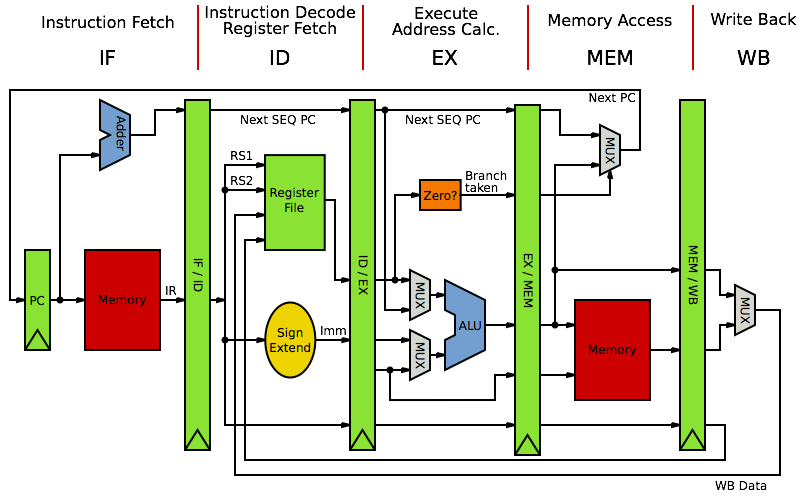
\includegraphics[width=1\textwidth]{img/MIPSarchitecture.png}
    \caption{MIPS architecture} %\protect\footnote{http://upload.wikimedia.org/wikipedia/commons/thumb/e/ea/MIPS\_Architecture(Pipelined).svg/300px-MIPS\_Architecture\_(Pipelined).svg.png}}
    \label{fig:MIPSarchitecture}
\end{figure}


\newpage

In this chapter, we will talk about the architecture components and assembly of MIPS 32-bit version.

\section{MIPS coprocessors}

MIPS was born for solving complex arithmetic problems by reducing the time consumed in those operations.
This is attained through the implementation of coprocessors within MIPS.

MIPS architecture includes four coprocessors respectively, CP0, CP1, CP2 and CP3:

\begin{enumerate}
\item Coprocessor 0, denoted by ~\textit{CP0}, is incorporated in the CPU chip; it supports the virtual memory system and exception handling (also known as the ~\textit{System Control Coprocessor}).
\item Coprocessor 1, denoted by ~\textit{CP1}, is reserved for floating point coprocessor.
\item Coprocessor 2, denoted by ~\textit{CP2}, is reserved for specific implementations.
\item Coprocessor 3, denoted by ~\textit{CP3}, is reserved for the implementations of the architecture.
\end{enumerate}

Notice that coprocessor ~\textit{CP0}, translates virtual addresses into physical addresses, manages exceptions, and handles switch between kernel, supervisor and user modes.

\section{MIPS cpu data formats}

The CPU of MIPS defines four differents formats:
\begin{itemize}
\item ~\textit{Bit} (1 bit, b)
\item ~\textit{Byte} (8 bits, B)
\item ~\textit{Halfword} (16 bits, H)
\item ~\textit{Word} (32 bits, W)
\end{itemize}




\section{MIPS registers usage}

MIPS architecture has 32 registers dedicated and there are some conventions to use those registers correctly.
Table ~\ref{tbl:compiler_register_usage} summarizes those registers, and their usage.


\begin{table}[h!]
\centering
\caption{MIPS registers}
\label{tbl:compiler_register_usage}
\begin{tabular}{cllc}
\hline
\multicolumn{1}{|c|}{\textbf{Name}} & \multicolumn{1}{c|}{\textbf{Number}} & \multicolumn{1}{c|}{\textbf{Use}}                                                                                                           & \multicolumn{1}{c|}{\textbf{\begin{tabular}[c]{@{}c@{}}Callee must\\  preserve?\end{tabular}}} \\ \hline
\multicolumn{1}{|c|}{\$zero}        & \multicolumn{1}{l|}{\$0}             & \multicolumn{1}{l|}{has constant 0}                                                                                                         & \multicolumn{1}{c|}{No}                                                                        \\ \hline
\multicolumn{1}{|c|}{\$at}          & \multicolumn{1}{l|}{\$1}             & \multicolumn{1}{l|}{register reserved for assembler (temporary)}                                                                            & \multicolumn{1}{c|}{No}                                                                        \\ \hline
\multicolumn{1}{|c|}{\$v0 - \$v1}     & \multicolumn{1}{l|}{\$2 - \$3}         & \multicolumn{1}{l|}{\begin{tabular}[c]{@{}l@{}}register reserved for returning values of functions,\\  and expression evaluation\end{tabular}} & \multicolumn{1}{c|}{No}                                                                        \\ \hline
\multicolumn{1}{|c|}{\$a0 - \$a3}     & \multicolumn{1}{l|}{\$4 - \$7}         & \multicolumn{1}{l|}{registers reserved for function arguments}                                                                              & \multicolumn{1}{c|}{No}                                                                        \\ \hline
\multicolumn{1}{|c|}{\$t0 - \$t7}     & \multicolumn{1}{l|}{\$8 - \$15}        & \multicolumn{1}{l|}{temporary registers}                                                                                                  & \multicolumn{1}{c|}{No}                                                                        \\ \hline
\multicolumn{1}{|c|}{\$s0 - \$s7}     & \multicolumn{1}{l|}{\$16 - \$23}       & \multicolumn{1}{l|}{saved temporary registers}                                                                                            & \multicolumn{1}{c|}{Yes}                                                                       \\ \hline
\multicolumn{1}{|c|}{\$t8 - \$t9}     & \multicolumn{1}{l|}{\$24 - \$25}       & \multicolumn{1}{l|}{temporary registers}                                                                                                  & \multicolumn{1}{c|}{No}                                                                        \\ \hline
\multicolumn{1}{|c|}{\$k0 - \$k1}     & \multicolumn{1}{l|}{\$26 - \$27}       & \multicolumn{1}{l|}{register reserved for OS kernel}                                                                                        & \multicolumn{1}{c|}{N/A}                                                                       \\ \hline
\multicolumn{1}{|c|}{\$gp}          & \multicolumn{1}{l|}{\$28}            & \multicolumn{1}{l|}{global pointer}                                                                                                         & \multicolumn{1}{c|}{Yes}                                                                       \\ \hline
\multicolumn{1}{|c|}{\$sp}          & \multicolumn{1}{l|}{\$29}            & \multicolumn{1}{l|}{stack pointer}                                                                                                          & \multicolumn{1}{c|}{Yes}                                                                       \\ \hline
\multicolumn{1}{|c|}{\$fp}          & \multicolumn{1}{l|}{\$30}            & \multicolumn{1}{l|}{frame pointer}                                                                                                          & \multicolumn{1}{c|}{Yes}                                                                       \\ \hline
\multicolumn{1}{|c|}{\$ra}          & \multicolumn{1}{l|}{\$31}            & \multicolumn{1}{l|}{return address}                                                                                                         & \multicolumn{1}{c|}{N/A}                                                                       \\ \hline
\multicolumn{4}{l}{\textit{Note: N/A (Not applicable)}}                                                                                                                                                                                                                                                                  
\end{tabular}
\end{table}

Table ~\ref{tbl:compiler_register_usage} is composed of 4 columns:

\begin{enumerate}
\item \textit{Name} displays the identifier of the registers available in MIPS. Those identifiers will be used as operands of MIPS instructions.
\item \textit{Number} column defines the number of each register. This number can also be used to refer to the register in an instruction.
\item \textit{Use} column refers to the meaning/definition of each register.
\item \textit{Callee must preserve?} column  provides information about the volatility of the register (used when a function is called).

\end{enumerate}

Beside those 32 registers, 3 more registers are dedicated to the CPU.

And they are known by:

\begin{itemize}

\item \textit{PC} - Program Counter register
\item \textit{HI} - Multiply and Divide register higher result
\item \textit{LO} - Multiply and Divide register lower result

\end{itemize}


\textit{PC} is the register which holds the address of the instruction that is being executed at the current time; ~\textit{HI} and ~\textit{LO} registers have different usage according to the instruction that is being executed.
In this case, let's see what context they have:
\begin{itemize}
\item when there is a multiply (~\textit{mul} instruction) operation, the \textit{HI} and  ~\textit{LO}  registers store the result of integer multiply.
\item when there is a multiply-add (~\textit{madd} instruction) or multiply-subtract (~\textit{msub} instruction) operation, the ~\textit{HI} and ~\textit{LO} register store the result of integer multiply-add or multiply-subtract.
\item when there is a division (~\textit{div} instruction) operation, the ~\textit{HI} register store the remainder of the division and the ~\textit{LO} register store the quotient of the division operation.
\item when there is a multiply-accumulate (~\textit{} instruction) operation, the ~\textit{HI} and ~\textit{LO} registers store the accumulated result of the operation.
\end{itemize}

See an overview of the MIPS registers in Figure ~\ref{fig:MIPS_register}.

\begin{figure}[h!]
  \centering
    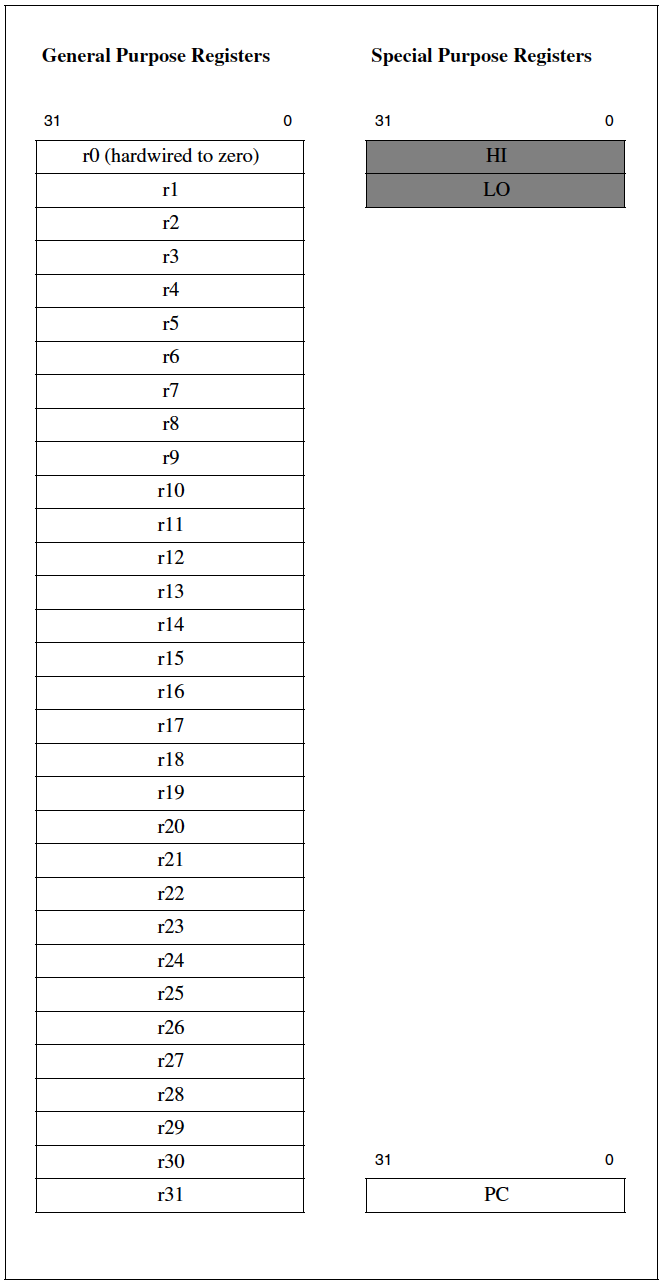
\includegraphics[scale=0.91]{img/mips_register.png}
    \caption{MIPS register}
    \label{fig:MIPS_register}
\end{figure}

\newpage



\section{MIPS instruction formats}
\label{sec:instruction_formats_mips}

Instructions, in MIPS, are divided into three types:
\begin{itemize}
\item R-Type
\item I-Type
\item J-Type
\end{itemize}

Each instruction is denoted by an unique mnemonic that represents the correspondent low-level machine instruction or operation.

Next sections provide the necessary details.

\subsection{MIPS R-Type}

R-Type instruction refers a register type instruction (it is the most complex type in MIPS).
The idea behind that instruction is to operate with registers only.

This type has the following format in MIPS (see Listing ~\ref{lst:r-type_format}).

\begin{lstlisting}[caption={R-Type instruction format},label={lst:r-type_format}]
  OP rd, rs, rt
\end{lstlisting}

In Listing ~\ref{lst:r-type_format}, the instruction is composed of one mnemonic, denoted by \textit{OP}, and three operands, denoted by ~\textit{rd} (destination register), ~\textit{rs} (source register), ~\textit{rt} (another source register).

The R-Type instruction format as the following mathematical semantics:

\begin{lstlisting}[caption={},label={}]
  rd = rs OP rt
\end{lstlisting}

To understand better this instruction, let's see an example of one R-Type instruction in MIPS (see Listing ~\ref{lst:example_r-type}).

\begin{lstlisting}[caption={Example of a R-Type instruction},label={lst:example_r-type}]
  add $t1, $t1, $t2
\end{lstlisting}

The instruction shown in Listing ~\ref{lst:example_r-type} means that register \$t1 shall be added (due to \textit{add} mnemonic) to register \$t2 and their sum (the result) stored in register \$t1.

The following equivalence explains that meaning.

\begin{align*}
  OP\ rd,\ rs,\ rt &\iff rd\ =\ rs\ OP\ rt\\
  &\makebox[\widthof{${}={}$}]{$\Downarrow$} \\
  add\ \$t1,\ \$t1,\ \$t2 &\iff \$t1\ =\ \$t1\ add\ \$t2 \\
  &\makebox[\widthof{${}={}$}]{$\Downarrow$} \\
  \$t1\ &=\ \$t1\ +\ \$t2
\end{align*}

Table ~\ref{tbl:r-type_binary_machine_code} defines the bit-structure of a R-Type instruction in a 32-bit machine.

\begin{table}[h!]
\centering
\caption{R-Type binary machine code}
\label{tbl:r-type_binary_machine_code}
\begin{tabular}{|c|c|c|c|c|c|}
\hline
\textbf{opcode} & \textbf{rs} & \textbf{rt} & \textbf{rd} & \textbf{shift (shamt)} & \textbf{funct} \\ \hline
6 bits          & 5 bits      & 5 bits      & 5 bits      & 5 bits                & 6 bits         \\ \hline
\end{tabular}
\end{table}

Let's explain each of the columns in Table ~\ref{tbl:r-type_binary_machine_code}.

\begin{itemize}
\item \textbf{opcode}  defines the instruction type. For every R-Type instruction, \textit{opcode} is set to the value 0. The \textit{opcode} field is 6 bits long (bit 31 to bit 26).
\item \textbf{rs} this is the first source register; it is the register where it will load the content of the register to the operation.The \textit{rs} field is 5 bits long (bit 25 to bit 21).
\item \textbf{rt} this is the second source register (same behaviour as \textit{rs} register). The \textit{rt} field is 5 bits long (bit 20 to bit 16).
\item \textbf{rd} this is the destination register; it is the register where the results of the operation will be stored. The \textit{rd} field is 5 bits long (bit 15 to bit 11).
\item \textbf{shift amount} the amount of bits to shift for shift instructions. The \textit{shift} field is 5 bits long (bit 10 to bit 6).
\item \textbf{function} specify the operation in addition to the \textit{opcode} field. The \textit{function} field is 6 bits long (bit 5 to bit 0).

\end{itemize}

Let's see an example of a R-Type instruction and its transformation to machine code in Table ~\ref{tbl:r-type_transformation2machine_code}.


\newpage

\begin{align*}
  add\ \$t0,&\ \$t0,\ \$t1\\
  &\makebox[\widthof{${}={}$}]{$\Downarrow$} \\
  add\ \$8,&\ \$8,\ \$9\\
  &\makebox[\widthof{${}={}$}]{$\Downarrow$} \\
  (8)_{10}\ =&\ (01000)_{2}\\
  (9)_{10}\ =&\ (01001)_{2}\\
  add\ instruction\ (fu&nct\ field)\ =\ (100000)_{2}\\
  &\makebox[\widthof{${}={}$}]{$\Downarrow$}
\end{align*}

\vspace{-7mm}
\begin{table}[h!]
\centering
\begin{tabular}{|l|l|l|l|l|l|}
\hline
\textbf{opcode (6bits)}      & \textbf{rs (5bits)}        & \textbf{rt (5bits)}        & \textbf{rd (5bits)}        & \textbf{shift (shamt) (5bits)} & \textbf{funct (6bits)}     \\ \hline
\multicolumn{1}{|c|}{000000} & \multicolumn{1}{c|}{01000} & \multicolumn{1}{c|}{01001} & \multicolumn{1}{c|}{01000} & \multicolumn{1}{c|}{00000}     & \multicolumn{1}{c|}{100000} \\ \hline
\end{tabular}
\caption{Transformation of R-Type instruction to machine code}
\label{tbl:r-type_transformation2machine_code}
\end{table}

In Table ~\ref{tbl:r-type_transformation2machine_code}, the instruction 'add \$t0, \$t0, \$t1' will be normalized with the name of the register according to the number associated for the register in MIPS (see Table ~\ref{tbl:compiler_register_usage}). Then a conversion operation is applied to the two register numbers (~\textit{8} and ~\textit{9}), translating them into their binary number with 5 bits long. Also we give the information for the ~\textit{add} instruction, which is set for the MIPS architecture (not predictable).


After that, we complete the table for R-Type instruction according to Table ~\ref{tbl:r-type_binary_machine_code} with the informations available and the restriction/rules associated to R-Type instruction in MIPS.

Notice that the ~\textit{opcode} field for R-Type instruction are set to the value 0 (according to the explanation in Table ~\ref{tbl:r-type_binary_machine_code}).

%Finally, we have our binary machine code for the instruction 'add \$t0, \$t0, \$t1' in Table ~\ref{tbl:r-type_transformation2machine_code}.

\subsection{MIPS I-Type}

I-Type instruction is a set of instructions which operate with an immediate value and a register value. 

Several different Immediate (~\textit{I-Type}) instructions formats are available.

Let's see those diferents formats for this type in Table ~\ref{tbl:I-Type_instruction_format}.

\begin{table}[h!]
\centering
\begin{tabular}{ccccll}
\multicolumn{1}{l|}{31 -- 26} & \multicolumn{1}{l|}{25 ---- 21} & \multicolumn{1}{l|}{20 -- 16} & \multicolumn{1}{l|}{15 -------- 11} & \multicolumn{1}{l|}{10 ------- 6} & 5 ----- 0                     \\ \hline
\multicolumn{1}{|c|}{opcode}  & \multicolumn{1}{c|}{rs}         & \multicolumn{1}{c|}{rt}       & \multicolumn{3}{c|}{immediate}                                                                          \\ \hline
\multicolumn{1}{|c|}{opcode}  & \multicolumn{1}{c|}{rd}         & \multicolumn{4}{c|}{offset}                                                                                                             \\ \hline
\multicolumn{1}{|c|}{opcode}  & \multicolumn{5}{c|}{offset}                                                                                                                                               \\ \hline
\multicolumn{1}{|c|}{opcode}  & \multicolumn{1}{c|}{rs}         & \multicolumn{1}{c|}{rt}       & \multicolumn{1}{c|}{rd}             & \multicolumn{2}{c|}{offset}                                       \\ \hline
\multicolumn{1}{|c|}{opcode}  & \multicolumn{1}{c|}{base}       & \multicolumn{1}{c|}{rt}       & \multicolumn{2}{c|}{offset}                                             & \multicolumn{1}{c|}{function} \\ \hline
\multicolumn{1}{l}{}          & \multicolumn{1}{l}{}            & \multicolumn{1}{l}{}          & \multicolumn{1}{l}{}                &                                   &                              
\end{tabular}
\caption{Distinct I-Type instruction formats}
\label{tbl:I-Type_instruction_format}
\end{table}

\newpage

In Table ~\ref{tbl:I-Type_instruction_format}, there are 5 differents instruction formats which corresponds to different bit structures as illustrated.

The most frequent MIPS I-Type instruction is the first one, denoted as Imm16 (Immediate instruction with 16 bits immediate value), is used for logical operands, arithmetic signed operands, load/store address byte offsets and PC-relative branch signed instruction displacements (see Table ~\ref{tbl:imm16_instruction}).

\begin{table}[h!]
\centering
\begin{tabular}{l|l|l|l}
31 --- 26                    & 25 --- 21               & 20 --- 16               & 15 ----------------- 0         \\ \hline
\multicolumn{1}{|c|}{opcode} & \multicolumn{1}{c|}{rs} & \multicolumn{1}{c|}{rt} & \multicolumn{1}{c|}{immediate} \\ \hline
\end{tabular}
\caption{Immediate (I-Type) Imm16 instruction format}
\label{tbl:imm16_instruction}
\end{table}

Let's see examples of Imm16 instruction:

\begin{lstlisting}
  addi $t0, $t0, 10 // Arithmetic operation
  ori $t0, $t1, 5   // Logical operation
  beq $t0, $t1, 1    // Conditional branch operation
  lw $t0, array1($t0) //Data transfer operation
\end{lstlisting}

The second instruction, denoted as Immediate Off21 instruction (Immediate instruction with 21bits offset), is used for comparing a register against zero and branch (offset field is larger than the usual 16-bit field (immediate field of the first instruction from the table above)).
See Table ~\ref{tbl:imm_off21_instruction}.

\begin{table}[h!]
\centering
\begin{tabular}{l|l|l|l}
31 --- 26                    & 25 --- 21               & \multicolumn{2}{l}{20 --------------------- 0} \\ \hline
\multicolumn{1}{|c|}{opcode} & \multicolumn{1}{c|}{rd} & \multicolumn{2}{c|}{offset}                     \\ \hline
\end{tabular}
\caption{Immediate (I-Type) Off21 instruction format}
\label{tbl:imm_off21_instruction}
\end{table} 

\begin{comment}
Let's see an example of Immediate Off21 instruction:
\begin{lstlisting}
  bltz $t0, jump
\end{lstlisting}
\end{comment}

The third instruction, denoted as Immediate Off26 instruction (Immediate instruction with 26 bits offset), is used for PC-relative branches with very large displacements (unconditional branches (BC mnemonic instruction) \& branch-and-link (BALC mnemonic instruction) with a 26-bit offset,).
See Table ~\ref{tbl:imm_off26_instruction}.

\begin{table}[h!]
\centering
\begin{tabular}{l|lll}
31 --- 26                    & \multicolumn{3}{l}{25 ------------------------------------ 0} \\ \hline
\multicolumn{1}{|c|}{opcode} & \multicolumn{3}{c|}{offset}                                   \\ \hline
\end{tabular}
\caption{Immediate (I-Type) Off26 instruction format}
\label{tbl:imm_off26_instruction}
\end{table}

The fourth instruction, denoted as Immediate Off11 instruction (Immediate instruction with 11 bits offset), is used for the newest encodings of coprocessor 2 load and store instructions (LWC2, SWC2, LDC2, SWC2).
See Table ~\ref{tbl:imm_off11_instruction_format}.

\begin{table}[h!]
\centering
\begin{tabular}{l|l|l|l|l}
31 --- 26                    & 25 ----- 21             & 20 --------- 16         & 15 ----------- 11       & 10 ------------------- 0    \\ \hline
\multicolumn{1}{|c|}{opcode} & \multicolumn{1}{c|}{rs} & \multicolumn{1}{c|}{rt} & \multicolumn{1}{c|}{rd} & \multicolumn{1}{c|}{offset} \\ \hline
\end{tabular}
\caption{Immediate (I-Type) Off11 instruction format}
\label{tbl:imm_off11_instruction_format}
\end{table}

Finally, the last one (fifth instruction), denoted as Immediate Off9 instruction (Immediate instruction with 9 bits offset), is used for SPECIAL3 instructions such as EVA memory access (~\textit{LBE} mnemonic). Also this is primarly used for instruction encodings that have been moved, such as ~\textit{LL} menmonic and ~\textit{SC} mnemonic instruction.
See Table ~\ref{tbl:imm_off9_instruction_format}.

\begin{table}[h!]
\centering
\begin{tabular}{l|l|l|l|l|l}
31 --- 26                    & 25 ----- 21               & 20 --------- 16         & 15 ------------------ 7     & 6 & 5 ------------------- 0       \\ \hline
\multicolumn{1}{|c|}{opcode} & \multicolumn{1}{c|}{base} & \multicolumn{1}{c|}{rt} & \multicolumn{1}{c|}{offset} & 0 & \multicolumn{1}{c|}{function} \\ \hline
\end{tabular}
\caption{Immediate (I-type) Off9 instruction format}
\label{tbl:imm_off9_instruction_format}
\end{table}

Notice that, for the project related to the thesis, only the first instruction type (Immediate (I-Type) Imm16 instruction format) was used. The other instruction formats are not really important for this project.


\subsection{MIPS J-Type}
J-Type instructions are instructions which jump to a certain address.
Let's see his format in Table ~\ref{tbl:j-type_instruction_format}.

\begin{table}[h!]
\centering
\begin{tabular}{l|l|l|l|l|l}
31 --- 26                    & \multicolumn{5}{l}{25 ----------------------------------------------------------------- 0} \\ \hline
\multicolumn{1}{|c|}{opcode} & \multicolumn{5}{c|}{address}                                                                \\ \hline
\end{tabular}
\caption{J-Type instruction format}
\label{tbl:j-type_instruction_format}
\end{table}

In Table ~\ref{tbl:j-type_instruction_format}, 6 bits are associated to the ~\textit{opcode} field and 26 bits for the ~\textit{address} field.
But notice that in MIPS, addresses are 32 bits long. 

For solving that, MIPS use a technique which leads to shift the address left by 2 bits and then combine 4 bits with the 4 high-order bits of the PC in front of the address.

Examples of J-Type formats can be seen in Listing ~\ref{lst:J-type_instruction}.

\begin{lstlisting}[caption={Examples of J-Type instruction},label={lst:J-type_instruction}]
  jal writeln  // Jump and link instruction
  jr $ra	 // Jump register instruction
  j writeln     // Jump instruction
\end{lstlisting}

In Listing ~\ref{lst:J-type_instruction}, we see three different types of jump instruction.
The first one example, is a ~\textit{jal} instruction and it means 'jump and link' in an extensive way. Basically, it jump to the branch written in front of the ~\textit{jal} nomenclature and stores the return address (instantly) to the return address register (\$ra; \$31). In this way, the programmer don't need to use some instructions for saving the return address and continue the flow of the execution code.

The second example, is a ~\textit{jr} instruction and it means 'jump to an address stored in a register'. Notice that registers are available in the MIPS architecture.

The third and last example is a ~\textit{j} instruction and this is a 'jump instruction'. Summing it up, it jumps to the branch written in front of the letter ~\textit{j}, which is in this case ~\textit{writeln}.



\section{MIPS assembly language}

MIPS language is divided into 2 parts (Data and Text parts).

\subsection{MIPS data declarations}

This section is used for declaring variable names used in the program.
Variables declared are allocated in the main memory (RAM) and must be identified with a particular nomenclature denoted as ~\textit{.data}. It is used for declaring global variables, principally.

Then comes the part when the variable names are declared.

Let's see the format for declaring a variable name in Listing ~\ref{lst:syntax_format_data_mips}.

\begin{lstlisting}[caption={Syntax format of data declarations in MIPS},label={lst:syntax_format_data_mips}]
  name: storage_type value(s)
\end{lstlisting}

In Listing ~\ref{lst:syntax_format_data_mips}, the ~\textit{name} field refers to the name of the variable. 

The ~\textit{storage\_type} refers to the type of the variable that can be:
\begin{itemize}
\item ~\textit{.ascii} store a string in memory without a null terminator.
\item ~\textit{.asciiz} store a string in memory with the null terminator.
\item ~\textit{.byte} store 'n' bytes contiguously in memory.
\item ~\textit{.halfword} store 'n' 16-bit halfwords contiguously in memory.
\item ~\textit{.word} store 'n' 32-bit words contiguously in memory.
\item ~\textit{.space} store a certain number of bytes of space in memory.
\end{itemize}

Lastly, the ~\textit{value(s)} field refers to the value of the type associated.

Let's see some example for declaring some variables in MIPS in Listing ~\ref{lst:data_declarations_examples_mips}.

\begin{lstlisting}[caption={Examples for declaring variables in MIPS},label={lst:data_declarations_examples_mips}]
  .data  # Tells assembler we're in the data segment
    val:  .word  10   
    str:  .ascii  "Hello, world"
    num:  .byte  0x01, 0x02
    arr:  .space 100
\end{lstlisting}

In Listing ~\ref{lst:data_declarations_examples_mips}, there are 4 different types under the ~\textit{data} section.

The variable ~\textit{val} contains the value '10' and the size of the variable is 32 bits.

The variable ~\textit{str} contains the string 'Hello World' and the size of the variable is the same size as the string.

The variable ~\textit{num} stores the listed value(s) (which appears after the ~\textit{.byte} nomenclature) as 8 bit bytes. In this example, it will be '0x00000201'.

The variable ~\textit{arr} reserves the next specified number of bytes in the memory, which will be 100 bytes reserved for that variable.




\subsection{MIPS text declarations}
This section contains the program code and follows a specific syntax starting with the keyword ~\textit{.text}.

As all programming languages, there is a starting point in the code that must be designated as ~\textit{main:}. Each of the assembly language statements in MIPS (written after the ~\textit{main:} field) are executed sequentially (excepted loop and conditional statements).

Let's see an example in Listing ~\ref{lst:text_declarations_mips}.

\begin{lstlisting}[caption={Example of Text declarations in MIPS},label={lst:text_declarations_mips}]
  .text 
    main:
      li $t0, 5
      li $t1, 10
      mul $t0, $t0, $t1
\end{lstlisting}

In Listing ~\ref{lst:text_declarations_mips}, we see the ~\textit{.text} which begins the code of the program and the ~\textit{main:} which shows where the code execution must start.

Below the keyword ~\textit{main:} appears all the instruction of the program code. 

In this case, it will load two numbers in different registers and multiply them (see Section ~\ref{sec:mips_instructions} to understand those instructions). 

Notice that the code will execute sequentially.

Also, in the text part beside of the code execution flow, we can write the name of branches for executing some jump instructions. This means that every jump instruction with a name associated, will see if that name is under the text part.
Like that when a jump instruction is available it can jump to the name associated.

%Also if some loop or conditional statements are available in MIPS, we need to know where the instructions for those conditions must be.
And for this purpose, we need to add some context to the MIPS jump instruction code and understand it better.



In this case, we need to replicate the same syntax as the ~\textit{main:} field but with the correct name of the condition or the loop (also inside of the text declarations parts). Like that, MIPS knows where it must jump for the next instruction.
Let's look an example in Listing ~\ref{lst:loop_mips}.

\begin{lstlisting}[caption={Example of a loop declaration in MIPS},label={lst:loop_mips}]
  .data 
  .text 
    main:
      li $t0, 5
      li $t1, 5
      mul $t0, $t0, $t1
      jal jump_condition #needs to jump to the field jump_condition
      li $t0, 4
      li $v0, 10
      syscall 
    jump_condition:  #syntax for jump and conditional instruction in mips
      li $t1, 5
      jr $ra
\end{lstlisting}

As we can see in Listing ~\ref{lst:loop_mips}, we have a ~\textit{jal} instruction available and a name associated next to the instruction. This name must be included under the ~\textit{.text} section, because the name is the name of the branch from where the jump instruction will jump. If the name isn't in the MIPS assembly code, then the program cannot execute the assembly code.
But in the example case, we can see that the name is available below as ~\textit{jump\_condition:}.
So this means that the ~\textit{jal} instruction will jump to that line and continue the code execution flow there.


Also, in MIPS, there is the possibility to include inline comments in the code using the symbol ~\textbf{\#}  on a line (see Listing ~\ref{lst:comments_mips}).

\begin{lstlisting}[caption={Example of a comment in MIPS},label={lst:comments_mips}]
  var1:		.word	3	# create a single integer variable with initial value 3
\end{lstlisting}

Let's see the template for a MIPS assembly language program in Listing ~\ref{lst:template_mips}.

\begin{lstlisting}[caption={Template of a MIPS assembly language},label={lst:template_mips}]
  # Comment giving name of program and description of function
  # Template.s
  # Bare-bones outline of MIPS assembly language program

    .data      # variable declarations follow this line
                  # ...
														
    .text       # instructions follow this line	
																	
      main:   # indicates start of code (first instruction to execute)
                  # ...
\end{lstlisting}








\section{MIPS instructions}
\label{sec:mips_instructions}
MIPS has 6 type of instructions :

\begin{itemize}
  \item instructions for data transfer
  \item instructions for arithmetic operations
  \item instructions for logical operations
  \item instructions for bitwise shift
  \item instructions for conditional branch
  \item instructions for unconditional branch
\end{itemize}

Let's see some examples of those instructions and their meanings.


\begin{table}[h!]
\centering
\caption{Example of Data transfer instruction in MIPS}
\label{tbl:data_transfer_instruction}
\begin{tabular}{|l|l|l|l|l|l|}
\hline
\multicolumn{1}{|c|}{\textbf{Name}} & \multicolumn{1}{c|}{\textbf{\begin{tabular}[c]{@{}c@{}}Instruction\\ Syntax\end{tabular}}} & \multicolumn{1}{c|}{\textbf{Meaning}} & \multicolumn{1}{c|}{\textbf{Format}} & \multicolumn{1}{c|}{\textbf{Opcode}} & \multicolumn{1}{c|}{\textbf{Funct}} \\ \hline
Store word                          & sw \$t,C(\$s)                                                                                & Memory[ \$s + C] = \$t                 & I                                    & \texttt{0x2B}                                                                                                    & N/A                                                                                                  \\ \hline
Load word                           & lw \$t,C(\$s)                                                                                & \$t = Memory[\$s + C]                 & I                                    & \texttt{0x23}                                                                                                    & N/A                                                                                                  \\ \hline
Load immediate                      & li \$t, C                                                                                  & \$t = C                               & I                                    & \texttt{0x9}                                                                                                     & N/A                                                                                                  \\ \hline
\end{tabular}
\end{table}


\begin{table}[h!]
\centering
\caption{Example of Arithmetic instruction in MIPS}
\label{tbl:arithmetic_instruction}
\begin{tabular}{|l|l|l|l|l|l|}
\hline
\multicolumn{1}{|c|}{\textbf{Name}}                          & \multicolumn{1}{c|}{\textbf{\begin{tabular}[c]{@{}c@{}}Instruction\\ Syntax\end{tabular}}} & \multicolumn{1}{c|}{\textbf{Meaning}}                                                                                                             & \multicolumn{1}{c|}{\textbf{Type}} & \multicolumn{1}{c|}{\textbf{Opcode}} & \multicolumn{1}{c|}{\textbf{Funct}} \\ \hline
Add                                                          & add \$d, \$s, \$t                                & \$d = \$s + \$t                                                                                                                                   & R                                    & \texttt{0x0}                                                                                                     & \texttt{0x20}                                                                                                   \\ \hline
\begin{tabular}[c]{@{}l@{}}Add\\ immediate\end{tabular}      & addi \$t, \$s, C                                   & \$t = \$s + C (signed)                                                                                                                              & I                                    & \texttt{0x8}                                                                                                     & N/A                                                                                                  \\ \hline
Subtract                                                     & sub \$d, \$s, \$t                                  & \$d = \$s - \$t                                                                                                                                     & R                                    & \texttt{0x0}                                                                                                     & \texttt{0x22}                                                                                                   \\ \hline
Move                                                    & move \$t0, \$t1                                                                              & \$t0 = \$t1                                                                                                                                         & R                                    & \texttt{0x0}                                                                                                     & \texttt{0x21}                                                                                                   \\ \hline
Multiply                                                & mul \$s, \$t, \$d                                                                            & \begin{tabular}[c]{@{}l@{}}\$s = \$t * \$d\\ LO = \$t * \$d (upper 32bits)\\ HI = \$t * \$d (lower 32bits)\end{tabular} & R                                    & \texttt{0x0}                                                                                                     & \texttt{0x19}                                                                                                   \\ \hline
Divide                                                  & div \$s, \$t, \$d                                                                            & \begin{tabular}[c]{@{}l@{}}\$s = \$t / \$d\\ LO = \$t / \$d\\ HI = \$t \% \$d\end{tabular}                              & R                                    & \texttt{0x0}                                                                                                     & \texttt{0x1A}                                                                                                   \\ \hline
\end{tabular}
\end{table}






\begin{table}[h!]
\centering
\caption{Example of Logical instruction in MIPS}
\label{tbl:logical_instruction}
\begin{tabular}{|l|l|l|l|l|l|}
\hline
\multicolumn{1}{|c|}{\textbf{Name}} & \multicolumn{1}{c|}{\textbf{\begin{tabular}[c]{@{}c@{}}Instruction\\ Syntax\end{tabular}}} & \multicolumn{1}{c|}{\textbf{Meaning}} & \multicolumn{1}{c|}{\textbf{Format}} & \multicolumn{1}{c|}{\textbf{Opcode}} & \multicolumn{1}{c|}{\textbf{Funct}} \\ \hline
Set on less than                    & slt \$d,\$s,\$t                                                                              & \$d = (\$s \textless \$t)               & R                                    & \texttt{0x0}                                                                                                     & \texttt{0x2A}                                                                                                   \\ \hline
Or                                  & or \$d,\$s,\$t                                                                               & \$d = \$s $\|$ \$t                         & R                                    & \texttt{0x0}                                                                                                     & \texttt{0x25}                                                                                                   \\ \hline
And                                 & and \$d,\$s,\$t                                                                              & \$d = \$s $\&$ \$t                        & R                                    & \texttt{0x0}                                                                                                     & \texttt{0x24}                                                                                                   \\ \hline
Set on less than unsigned           & sltu \$d,\$s,\$t                                                                             & \$d = (\$s \textless \$t)               & R                                    & \texttt{0x0}                                                                                                     & \texttt{0x2B}                                                                                                   \\ \hline
Exclusive or immediate              & xori \$d,\$s,C                                                                                & \$d = \$s \textasciicircum  C           & I                                    & \texttt{0xE}                                                                                                     & N/A                                                                                                  \\ \hline
\end{tabular}
\end{table}




\begin{table}[h!]
\centering
\caption{Example of Bitwise Shift instruction in MIPS}
\label{tbl:bitwise_shift_instruction}
\begin{tabular}{|l|l|l|l|l|l|}
\hline
\multicolumn{1}{|c|}{\textbf{Name}}                                      & \multicolumn{1}{c|}{\textbf{\begin{tabular}[c]{@{}c@{}}Instruction\\ Syntax\end{tabular}}} & \multicolumn{1}{c|}{\textbf{Meaning}}  & \multicolumn{1}{c|}{\textbf{Format}} & \multicolumn{1}{c|}{\textbf{Opcode}} & \multicolumn{1}{c|}{\textbf{Funct}} \\ \hline
\begin{tabular}[c]{@{}l@{}}Shift left logical \\ immediate\end{tabular}  & sll \$d,\$t,shamt                                                                            & \$d = \$t \textless\textless shamt       & R                                    & \texttt{0x0}                                                                                                     & \texttt{0x0}                                                                                                    \\ \hline
\begin{tabular}[c]{@{}l@{}}Shift right logical \\ immediate\end{tabular} & srl \$d,\$t,shamt                                                                            & \$d = \$t \textgreater\textgreater shamt & R                                    & \texttt{0x0}                                                                                                     & \texttt{0x2}                                                                                                    \\ \hline
Shift left logical                                                       & sllv \$d,\$t,\$s                                                                             & \$d = \$t \textless\textless \$s         & R                                    & \texttt{0x0}                                                                                                     & \texttt{0x4}                                                                                                    \\ \hline
Shift right logical                                                      & srlv \$d,\$t,\$s                                                                             & \$d = \$t \textgreater\textgreater \$s   & R                                    & \texttt{0x0}                                                                                                     & \texttt{0x6}                                                                                                    \\ \hline
\end{tabular}
\end{table}


\begin{table}[h!]
\centering
\caption{Example of Conditional Branch instruction in MIPS}
\label{tbl:conditional_branch_instruction}
\begin{tabular}{|l|l|l|l|l|l|}
\hline
\multicolumn{1}{|c|}{\textbf{Name}}                             & \multicolumn{1}{c|}{\textbf{\begin{tabular}[c]{@{}c@{}}Instruction\\ Syntax\end{tabular}}} & \multicolumn{1}{c|}{\textbf{Meaning}}                                    & \multicolumn{1}{c|}{\textbf{Format}} & \multicolumn{1}{c|}{\textbf{Opcode}} & \multicolumn{1}{c|}{\textbf{Funct}} \\ \hline
\begin{tabular}[c]{@{}l@{}}Branch if equal \\ zero\end{tabular} & beqz \$s, jump                                                                             & \begin{tabular}[c]{@{}l@{}}if(\$s==0) go to \\ jump address\end{tabular} & I                                    & \texttt{0x4}                                                                                                     & N/A                                                                                                  \\ \hline
\begin{tabular}[c]{@{}l@{}}Branch on not \\ equal\end{tabular}  & bne \$s, \$t, C                                                                              & \begin{tabular}[c]{@{}l@{}}if (\$s != \$t) go to \\ PC+4+4*C\end{tabular}  & I                                    & \texttt{0x5}                                                                                                     & N/A                                                                                                  \\ \hline
Branch on equal                                                 & beq \$s, \$t,C                                                                                & \begin{tabular}[c]{@{}l@{}}if (\$s == \$t) go to \\ PC+4+4*C\end{tabular}  & I                                    & \texttt{0x4}                                                                                                     & N/A                                                                                                  \\ \hline
\end{tabular}
\end{table}


\begin{table}[h!]
\centering
\caption{Example of Unconditional Branch instruction in MIPS}
\label{tbl:unconditional_branch_instruction}
\begin{tabular}{|l|l|l|l|l|l|}
\hline
\multicolumn{1}{|c|}{\textbf{Name}} & \multicolumn{1}{c|}{\textbf{\begin{tabular}[c]{@{}c@{}}Instruction\\ Syntax\end{tabular}}} & \multicolumn{1}{c|}{\textbf{Meaning}}                                                     & \multicolumn{1}{c|}{\textbf{Format}} & \multicolumn{1}{c|}{\textbf{Opcode}} & \multicolumn{1}{c|}{\textbf{Funct}} \\ \hline
Jump                                & j target                                                                                        & PC = PC+4{[}31:28{]} . target*4                                                                & J                                    & \texttt{0x2}                                                                                                     & N/A                                                                                                  \\ \hline
Jump register                       & jr \$s                                                                                     & goto address \$s                                                                          & R                                    & \texttt{0x0}                                                                                                     & \texttt{0x8}                                                                                                    \\ \hline
Jump and link                       & jal target                                                                                      & \begin{tabular}[c]{@{}l@{}}\$31 (\$ra) = PC + 4; \\ PC = PC+4{[}31:28{]} . target*4\end{tabular} & J                                    & \texttt{0x3}                                                                                                     & N/A                                                                                                  \\ \hline
\end{tabular}
\end{table}

\newpage
Some explanation must be provided for understanding the tables shown previously:
\begin{itemize}
\item ~\textbf{PC} means Program Counter.
\item ~\textbf{target} means the name of the target (used for jump instructions).
\item ~\textbf{C} means constants.
\item ~\textbf{\texttt{0x..}} means a hexadecimal format number.
\item ~\textbf{N/A} means Not Applicable.
\item ~\textbf{shamt} means the number to shift (used in shift instructions).
\end{itemize} 
Note that the ~\textit{Format}, ~\textit{ Opcode} and ~\textit{Funct} are the information of each field for each format instruction as explained in Section ~\ref{sec:instruction_formats_mips}.

Beside those instructions, some others instructions are sequences of instructions and they are called as pseudo instructions (see in Table ~\ref{tbl:pseudo_instructions}).


\begin{table}[h!]
\centering
\caption{Example of Pseudo Instructions in MIPS}
\label{tbl:pseudo_instructions}
\begin{tabular}{|l|l|l|l|l|l|}
\hline
\multicolumn{1}{|c|}{\textbf{Name}}       & \multicolumn{1}{c|}{\textbf{\begin{tabular}[c]{@{}c@{}}Instruction\\ Syntax\end{tabular}}} & \multicolumn{1}{c|}{\textbf{Real instruction translation}}                                          & \multicolumn{3}{c|}{\textbf{Meaning}}     \\ \hline
Move                                      & move \$d, \$s                                                                                & add \$d, \$s, \$zero                                                                                  & \multicolumn{3}{l|}{\$d=\$s}                \\ \hline
Load Address                              & la \$d, LabelAddr                                                                          & \begin{tabular}[c]{@{}l@{}}lui \$d, LabelAddr{[}31:16{]}\\ ori \$d, \$d, LabelAddr{[}15:0{]}\end{tabular} & \multicolumn{3}{l|}{\$d = Label Address}  \\ \hline
\begin{tabular}[c]{@{}l@{}}Multiplies and \\ returns only first \\ 32 bits\end{tabular} & mul \$d, \$s, \$t                                                                            & \begin{tabular}[c]{@{}l@{}}mult \$s, \$t\\ mflo \$d\end{tabular}                                      & \multicolumn{3}{l|}{\$d = \$s * \$t}        \\ \hline
\begin{tabular}[c]{@{}l@{}}Divides and \\ returns quotient\end{tabular}               & div \$d, \$s, \$t                                                                            & \begin{tabular}[c]{@{}l@{}}div \$s, \$t\\ mflo \$d\end{tabular}                                       & \multicolumn{3}{l|}{\$d = \$s / \$t}        \\ \hline
\begin{tabular}[c]{@{}l@{}}Branch if equal \\ to zero\end{tabular}                   & beqz \$s, Label                                                                            & beq \$s, \$zero, Label                                                                                & \multicolumn{3}{l|}{if (\$s==0) PC=Label} \\ \hline
\end{tabular}
\end{table}

Additionally, MIPS includes a number of system services for input and output interaction, denoted as ~\textbf{SYSCALL}.
Let's see an example of those services in Table ~\ref{tbl:syscall_mips}.

\begin{table}[h!]
\centering
\caption{Example of SYSCALL instruction in MIPS}
\label{tbl:syscall_mips}
\begin{tabular}{|l|c|l|l|}
\hline
\multicolumn{1}{|c|}{\textbf{Service}}                                & \textbf{\begin{tabular}[c]{@{}c@{}}Code in\\ \$v0\end{tabular}} & \multicolumn{1}{c|}{\textbf{Arguments}}                                                      & \multicolumn{1}{c|}{\textbf{Result}}                                                 \\ \hline
print integer                                                         & 1                                                               & \$a0 = integer to print                                                                      &                                                                                      \\ \hline
print string                                                          & 4                                                               & \begin{tabular}[c]{@{}l@{}}\$a0 = address of null-\\ terminated string to print\end{tabular} &                                                                                      \\ \hline
read integer                                                          & 5                                                               &                                                                                              & \$v0 contains integer read                                                           \\ \hline
\begin{tabular}[c]{@{}l@{}}sbrk (allocate\\ heap memory)\end{tabular} & 9                                                               & \begin{tabular}[c]{@{}l@{}}\$a0 = number of bytes to\\  allocate\end{tabular}                & \begin{tabular}[c]{@{}l@{}}\$v0 contains address of\\  allocated memory\end{tabular} \\ \hline
\begin{tabular}[c]{@{}l@{}}exit (terminate\\ execution)\end{tabular}  & 10                                                              &                                                                                              &                                                                                      \\ \hline
\end{tabular}
\end{table}

To understand better Table ~\ref{tbl:syscall_mips}, we need to give some explanation of it.
The ~\textit{service} column gives us the context of the service; the ~\textit{code} column explains which value must be set into register \$v0 (associated to the service wished); the ~\textit{arguments} column specify the argument values that must be loaded depending on the service and lastly; the ~\textit{result} column gives some informations about the return value of the service (if available or not).

Let's see an example of one service in Listing ~\ref{lst:printing_integer_mips}.

\begin{lstlisting}[caption={Example of printing integer in MIPS},label={lst:printing_integer_mips}]
  li $t0, 3             #adding the number 3 to register t0
  li  $v0, 1           # loading the service number 1 (print integer) to register v0
  add $a0, $t0, $zero  # loading the argument value to register a0
  syscall  #calling the syscall for printing the integer.
\end{lstlisting}




Notice that every instructions shown in the tables, are instructions which were used for the project.

\section{MIPS Memory Management}

MIPS has the possibility to control and coordinate the computer memory by two ways:
\begin{enumerate}
\item stack
\item heap
\end{enumerate}

\subsection{MIPS stack}
When a program is being executed, a portion of memory is set aside for the program and it is called the ~\textbf{stack}.

The stack is used for functions and it set some spaces for local variables of the functions.

Internally, MIPS doesn't have real instructions for pushing or popping the stack.
But this can be made with a sequences of instructions and using the stack pointer register.

Let's see an example in Listing ~\ref{lst:push_pop_mips}.

\begin{lstlisting}[caption={Example of push and pop instructions in MIPS},label={lst:push_pop_mips}]
  push:  addi $sp, $sp, -4  # Decrement stack pointer by 4
         sw   $v0, 0($sp)   # Save register v0 to stack

  pop:  lw   $v0, 0($sp)   # Copy from stack to register v0
        addi $sp, $sp, 4   # Increment stack pointer by 4
\end{lstlisting}

\subsection{MIPS heap}
Beside a stack, we might need to allocate some dynamic memory.
And this can be done by using a ~\textbf{Heap}.

For this purpose, in MIPS, we only need to say how much bytes we want to allocate in the heap.

Let's see an example in Listing ~\ref{lst:heap_mips}.

\begin{lstlisting}[caption={Example of code for allocating in the heap}, label={lst:heap_mips}]
.text 
  main:
    li $a0, 4 #we want to allocate 4 bytes in the heap.
    li $v0, 9 # we load the value 9 in register v0 for calling the heap instruction.
    syscall   # calling the system call instruction for allocating 4 bytes into the heap. The register v0 contains the address of allocated memory.
\end{lstlisting}

\section{MIPS simulator}

Several simulators are available in the market for executing MIPS assembly code, and some are free.

For this project, we considered two nice free simulators:
\begin{itemize}
\item MARS simulator \footnote{\url{http://courses.missouristate.edu/KenVollmar/MARS/}}
\item SPIM simulator \footnote{\url{http://spimsimulator.sourceforge.net}}
\end{itemize}

Both simulators are for education purposes and built with a GUI.

They execute and debug MIPS assembly code but only MARS simulator has the possibility to write some live-code MIPS assembly code. This explains why MARS was the one selected for this project.

\subsection{MARS at a glance}

MARS from ~\textit{Mips Assembly and Runtime Simulator}, assembles and simulates the execution of MIPS assembly language programs. The strength of MARS comes from the interaction between the user and the program through its integrated development environment (IDE) and the tools available there (program editing, assembling code, interactive debugging...).

Let's see MARS IDE in Figure ~\ref{fig:MARS_GUI}.

\begin{figure}[h!]
  \centering
    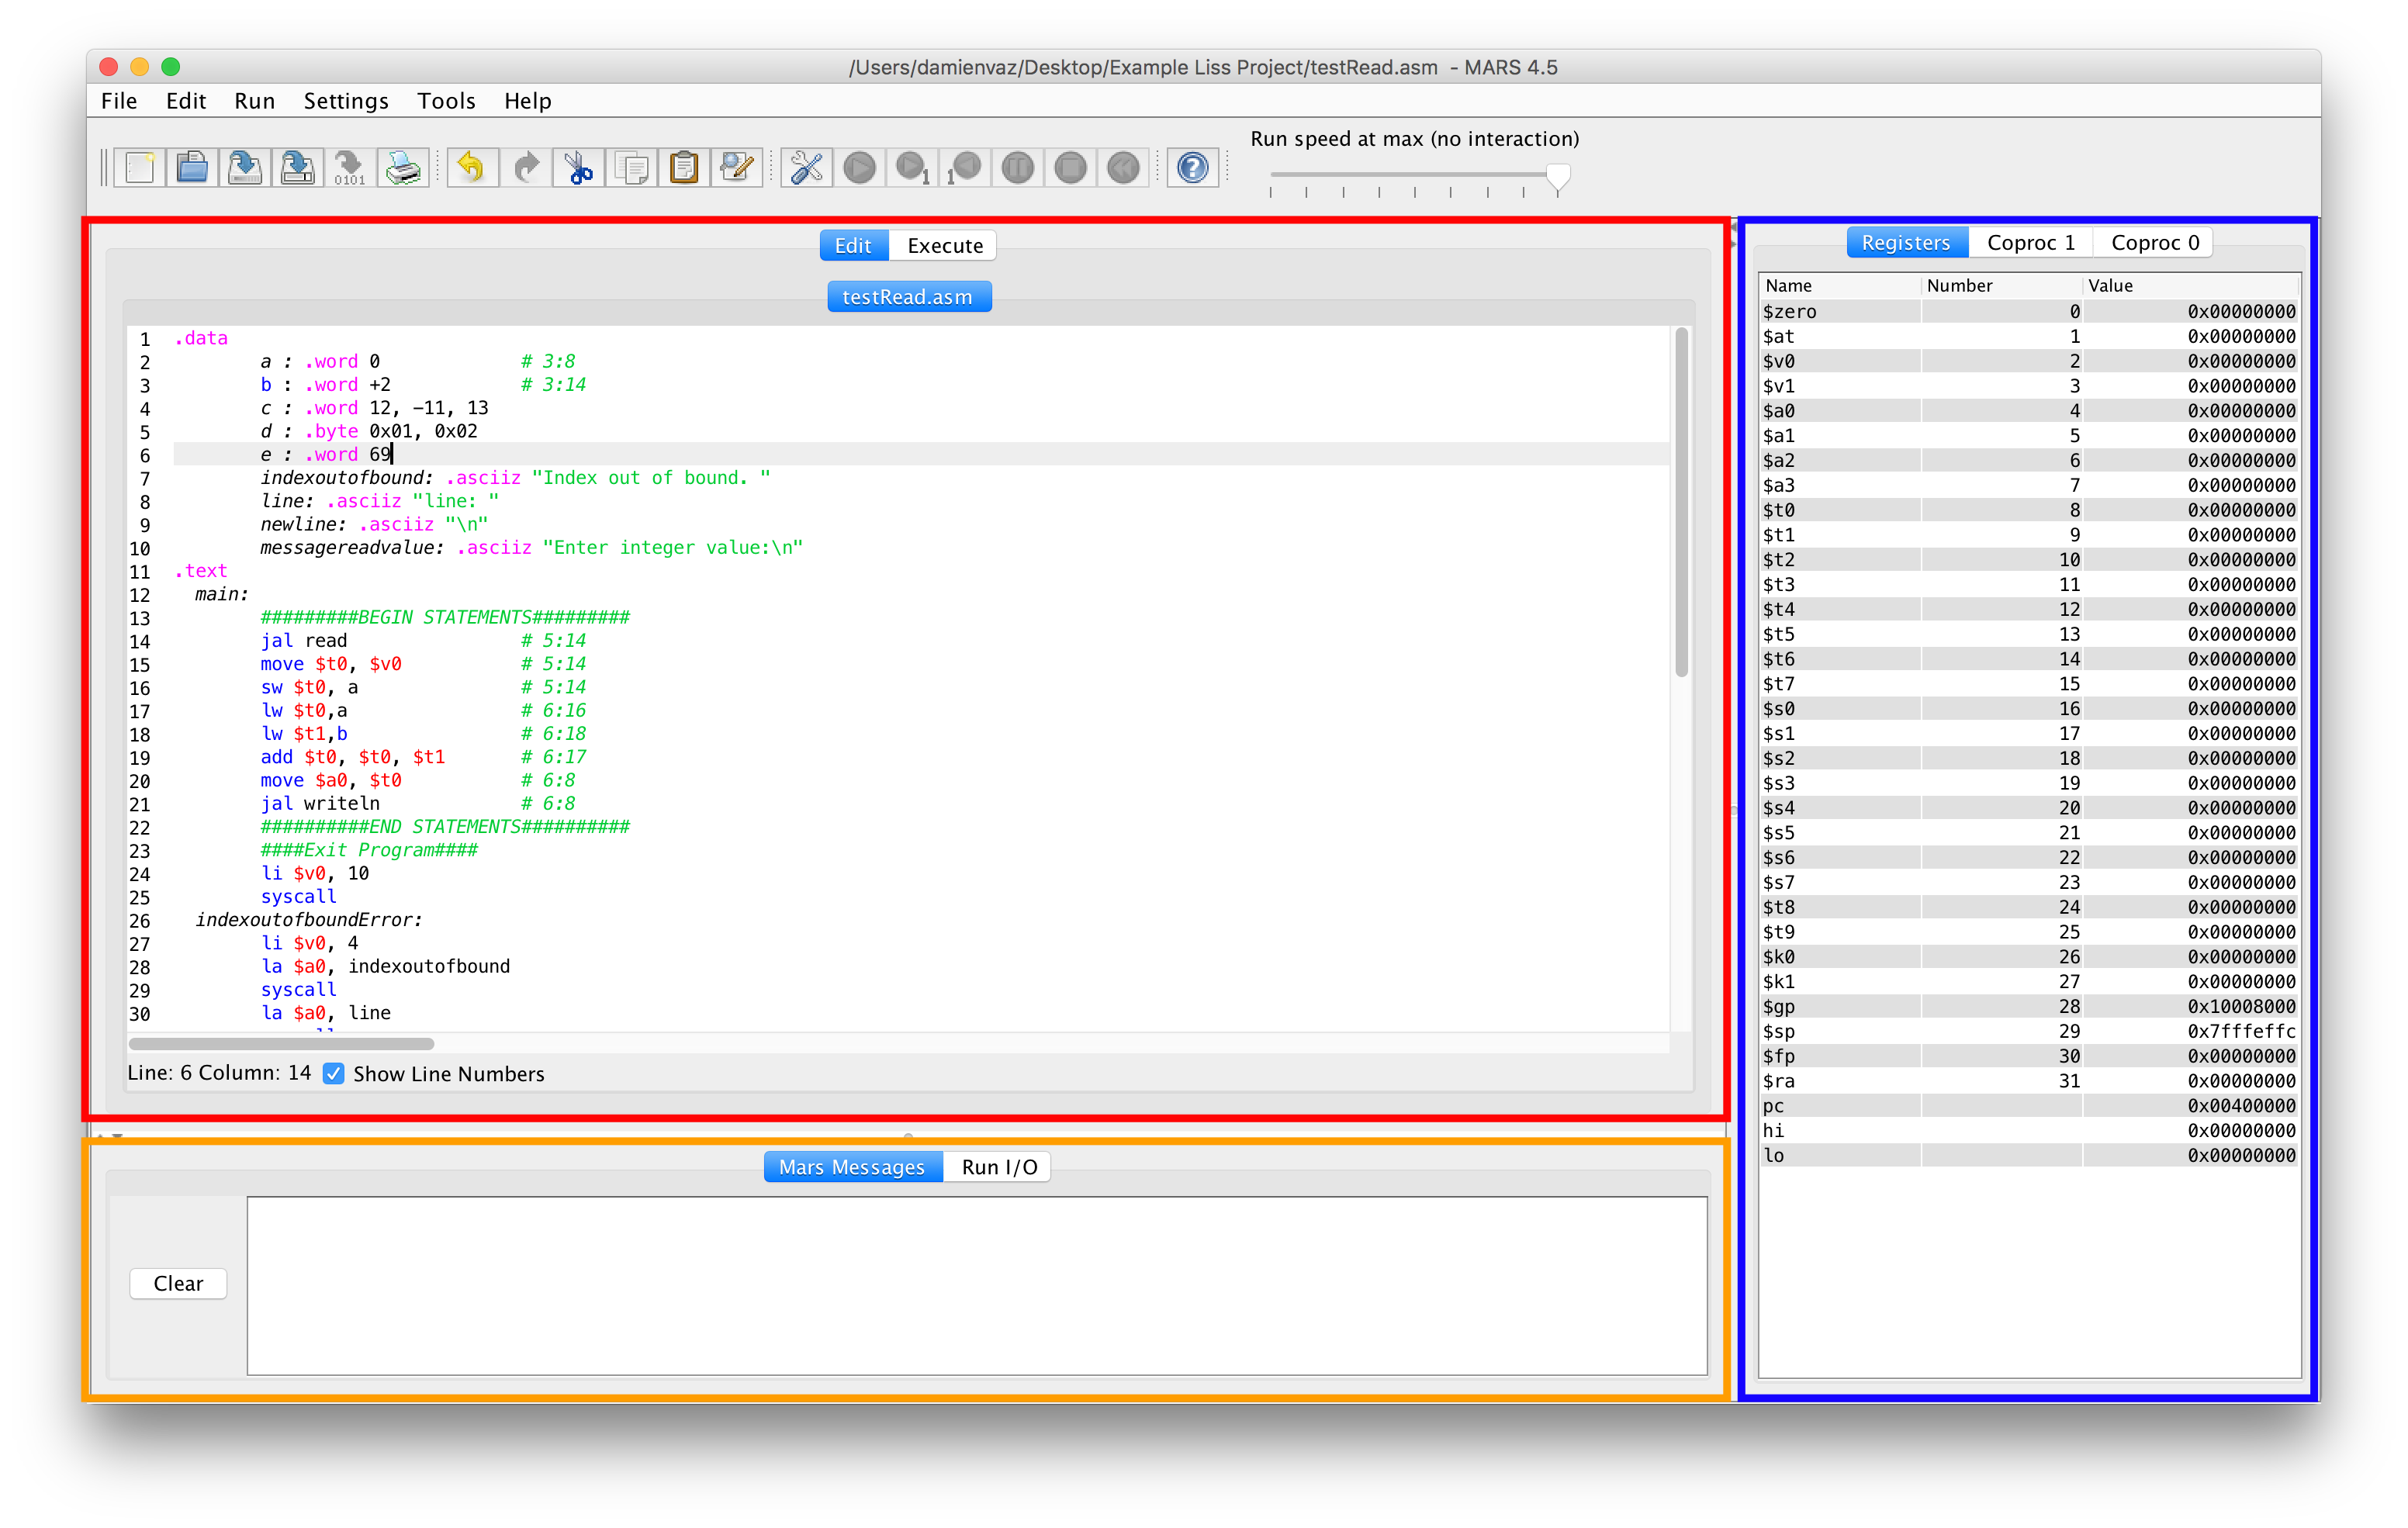
\includegraphics[width=1\textwidth]{img/MARS_GUI.png}
    \caption{MARS GUI}
    \label{fig:MARS_GUI}
\end{figure}

In Figure ~\ref{fig:MARS_GUI}, we have 3 different boxes.
The red box offers two possible views (two different perspective by switching between the tabs available at the top).
In this case, the view is opened for programing some live MIPS assembly code (MIPS assembly code is colored along the left part of the window).
But if we open the second tab view, then it will change to the execution mode of the MIPS assembly code (if no syntatic or semantic errors are found).

The orange box also has two possible views (Mars Messages or Run I/O tabs). It is used to display error messages regarding the syntax and semantic of MIPS assembly code, or error messages regarding the execution of the MIPS assembly code.

Lastly, the blue box has three different views: Registers, Co-processor1 and Co-processor 2. In the Figure above, it shows the states of the registers available in MIPS architecture but if we change the view it can show the states of each co-processor (related to division, multiplication).


If the MIPS assembly code typed in (or loaded from a file) is correct (no errors detected), we can assemble it and execute it.

Figure ~\ref{fig:MARS_GUI_EXECUTE} illustrates the new view offered by the IDE after assembling the source program.

\begin{figure}[h!]
  \centering
    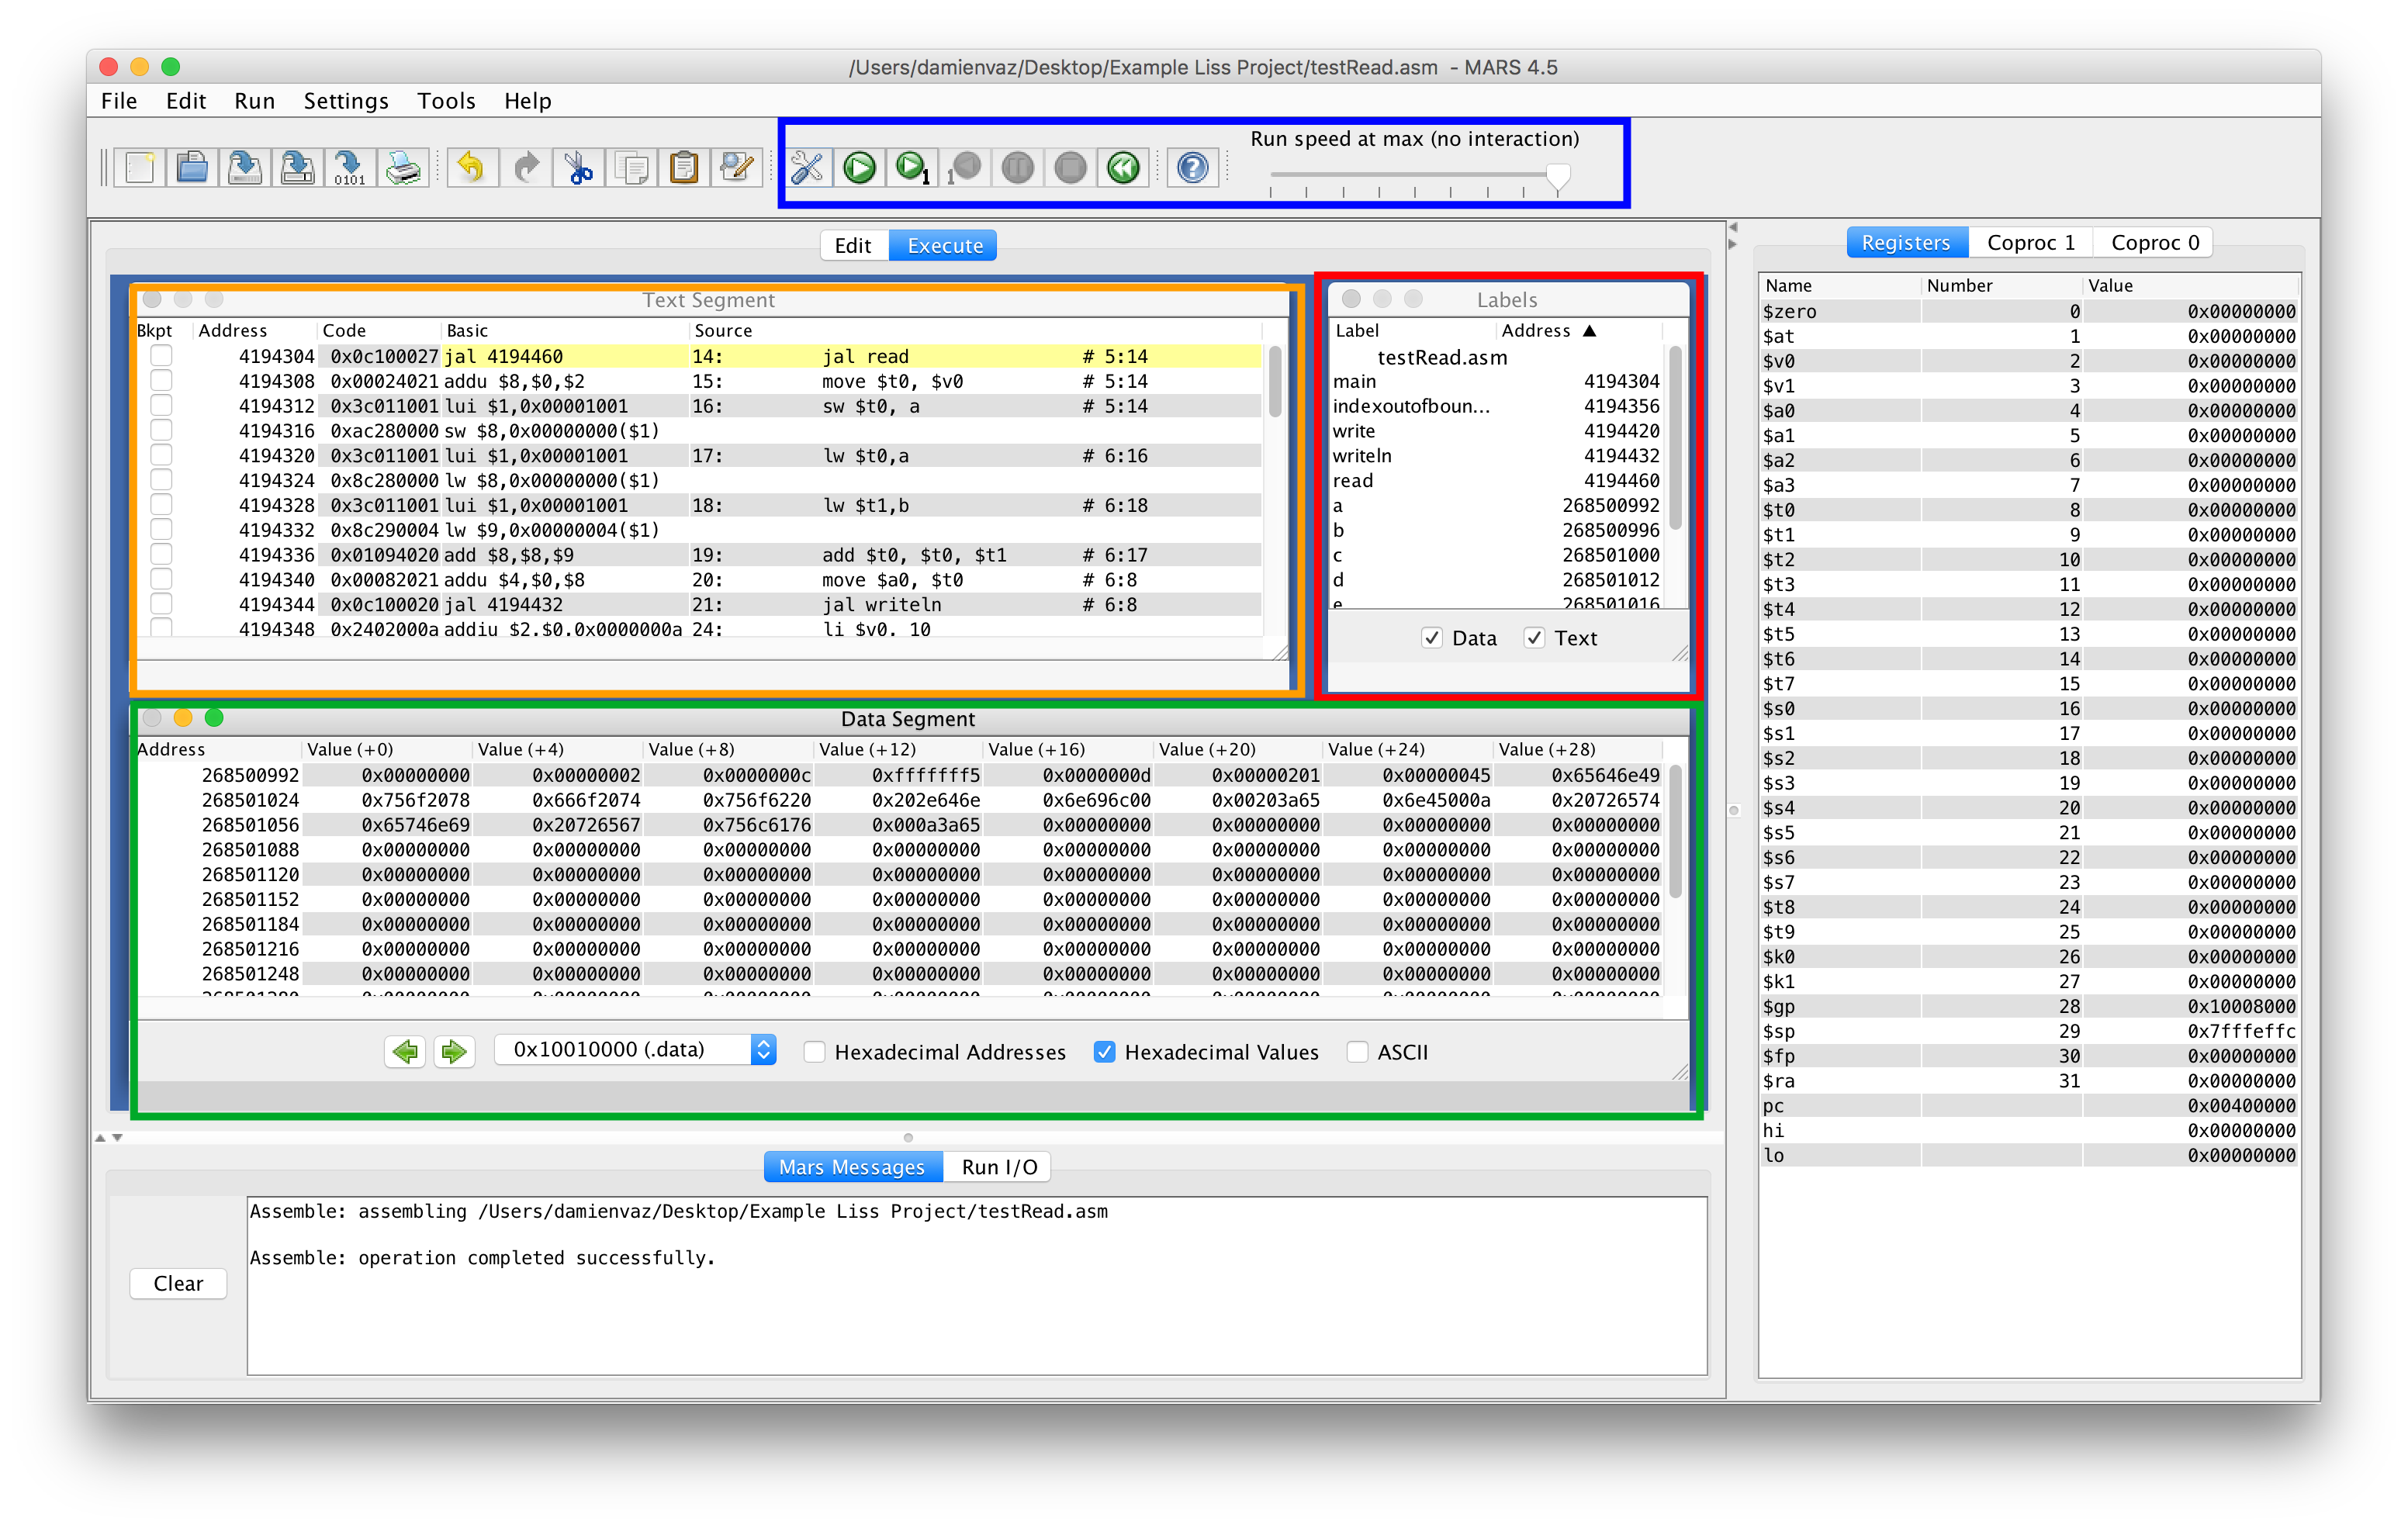
\includegraphics[width=1\textwidth]{img/MARS_GUI_EXECUTE.png}
    \caption{MARS GUI (Execution mode)}
    \label{fig:MARS_GUI_EXECUTE}
\end{figure}

In Figure ~\ref{fig:MARS_GUI_EXECUTE},  it is possible to identify the main window (the red one in Figure ~\ref{fig:MARS_GUI}) now split into three subwindows: orange, red and green. 

Notice that above the main red window, a small blue box contains buttons to activate tools for assembling MIPS assembly code, executing MIPS assembly code totally or step by step (one instruction at a time) and also the possibility to change the speed execution of the MIPS assembly code if we want to run it completely.

The orange box contains the MIPS assembly code assembled and ready to execute. It shows the MIPS assembly code instructions, the correspondent code in hexadecimal, the respective address in the memory, and eventually some breakpoints associated with certain MIPS assembly instructions. Also notice that MIPS assembly code has some pseudo-instructions; and in the orange box, there is a part where we can see the translation of the MIPS assembly code to another lower MIPS assembly code ( with no pseudo-instruction).
The yellow bar, or cursor, displayed in the figure above enhances the next instruction to be executed.

The red box is the identifier table for the MIPS assembly code. It contains the variables existing in the MIPS assembly code and displays their respective address in the memory.

The green box represents the virtual memory of the MIPS architecture. It displays the stack and the heap memory, as well as other informations not relevant in this context. Basically, we see the value being changed throw the iteration of the MIPS assembly code being executed. This mean that if there is a store instruction for a certain variable, it will look up for the identifer table (red box), search the address associated to the variable and store to that address the value associated to the variable.


\newpage

%%%%%%%%%%%%%%%%%%%%%%%%%%%%%%%%%%%%%%%%%%%%%%%%%%%%

\begin{comment}

As mentioned in the previous section, the AG processed by the compiler generator ANTLR will compose MIPS assembly. The MIPS assembly instructions generated so far will be converted into executable machine code by an assembler included in MARS environment (a MIPS simulator and debugger) according to the process depicted in Figure ~\ref{fig:hl2ll}.


\begin{figure}[h!]
  \centering
    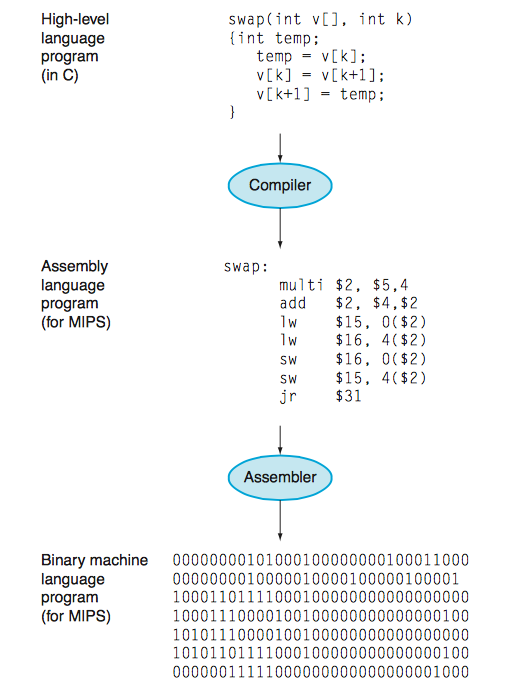
\includegraphics[height=0.9\textwidth]{img/high-level-2-low-level.png}
    \caption{Stages converting high-level language into binary machine language \protect\footnote{\cite{DAPJLH}}}
    \label{fig:hl2ll}
\end{figure}



%\section{Citations}
%Example of a citation: \cite{GRM97}, cf.\ this entry in the \Bibtex\ file.
%Another way of citing is \citep{KeR88}

%\section{Optional}
%You may wish to use the \conexp{Concept-Explorer} tool.

%\chapter{The problem and its challenges}


After presenting in the previous chapter the essential definitions for the intended work, in this chapter the project planned for this master thesis will be explained.

%Firstly, there is the necessity of generating the GIC from LISS language, like that we will see if there is no problem with the rules and definitions of a well grammar and follow the same grammar as LISS language (not being distinct) using ANTLR tool.

First, create an ANTLR version of the CFG grammar for LISS language.


Second, extend the LISS CFG to an AG in order to specify throw it the generation of MIPS assembly code.
To verify the correctness of the assembly code generated, a simple MIPS simulator, named MARS, will be selected to provide all the tools for checking it.

Third, the desired Structure-Editor, SDE, will be developed based on ANTLR.
It will be implemented in with Java SWING because ANTLR has always been implemented via Java and it is said, also, to use Java target as a reference implementation mirrored by other targets.
SWING is a GUI widget toolkit for Java which provides all the API for creating an interface with Java.
At this phase, we will create an IDE similar to other platforms but with the capacity of being a syntax-directed editor.

Fourthly, to complete the SDE functionality, an incremental compiler shall be included.
Incremental compilation ~\citep{RTD83a,Hol87a,VSK90a} means that only the part that was changed must be processed again. And like that, both tasks (edition and compilation) are done synchronously at the same time and having an editor which compiles cleverly.

Finally, exhaustive and relevant tests will be made with the tool created and, the outcomes will be analyzed and discussed.

%\section*{LISS language}


%\section{Assembly code MIPS}

%que se deve falar ?

%         The problem and its challenges.

%\section{Images}
%       Example of inserting an image as displyed text,
%\begin{center}
%       
\includegraphics[width=0.2\textwidth]{img/mei-logo-03.jpg}
%\end{center}

%\begin{wrapfigure}{r}{0.25\textwidth}
%       
\includegraphics[width=0.2\textwidth]{img/mei-logo-03.jpg}
%\end{wrapfigure}
%\noindent --- wrapped into the text,
%bla-bla bla-bla bla-bla bla-bla bla-bla bla-bla bla-bla bla-bla bla-bla bla-bla
%bla-bla bla-bla bla-bla bla-bla bla-bla bla-bla bla-bla bla-bla bla-bla bla-bla
%bla-bla bla-bla bla-bla bla-bla bla-bla bla-bla bla-bla bla-bla bla-bla bla-bla
%bla-bla bla-bla bla-bla bla-bla bla-bla bla-bla bla-bla bla-bla bla-bla bla-bla
%bla-bla bla-bla bla-bla bla-bla bla-bla bla-bla bla-bla bla-bla bla-bla bla-bla bla-bla bla-bla bla-bla bla-bla
%bla-bla bla-bla bla-bla bla-bla bla-bla bla-bla bla-bla bla-bla bla-bla bla-bla bla-bla bla-bla bla-bla bla-bla

%\noindent --- or as a floating body.
%\begin{figure}
%\begin{center}
%       
\includegraphics[width=0.5\textwidth]{img/mei-logo-03.jpg}
%\end{center}
%\caption{caption}
%\end{figure}

%You can also use an image as an icon, eg.\ \MEI, in the main tex.
%Click on it to visit the website. It is also listed in the list of terms.
%Another example of an item to appear in the term index: \UM (needs \Makeindex)


%\part{Core of the dissertation}

%\part{Core of the dissertation}

\end{comment}

%%%%%%%%%%%%%%%%%%%%%%%%%%%%%%%%%%%%%%%%%%%%%%%%%%%%%%%%%%%%%

\chapter{Compiler development}
%       Main result(s) and their scientific evidence
%\section{Introduction}
Earlier in the history of computers, software was primarily written in assembly language. Due to the low productivity of programming assembly code, researchers invented a way that add some more productivity and flexibility for programmers; they created the compiler allowing to wire programs in high level programming languages.

A compiler is a software program which converts a high-level programming language (source code) into a lower level programing language for the target machine (known as machine code or assembly language).

The compiler task is divided into several steps (see Figure ~\ref{fig:compiler}):
\begin{enumerate}
  \item Lexical analysis
  \item Syntactic analysis or parsing
  \item Semantic analysis
  \item Optimization
  \item Code generation
\end{enumerate}

\begin{figure}
\begin{center}
       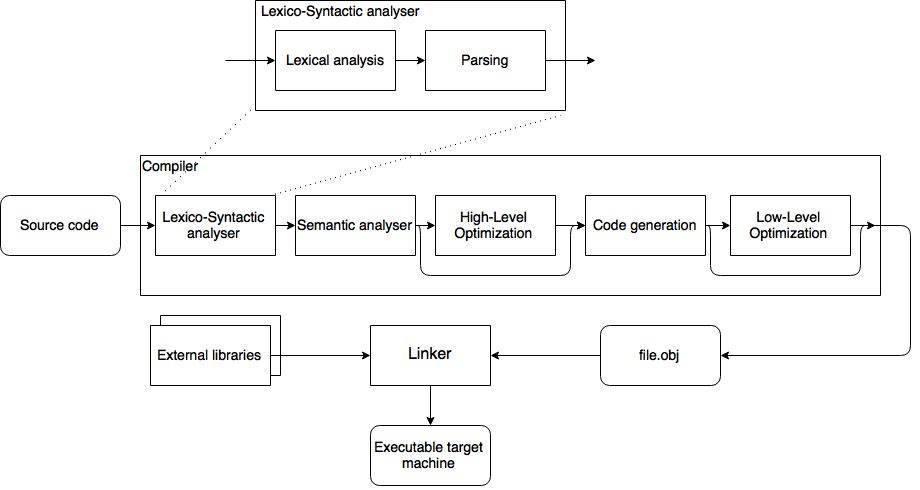
\includegraphics[width=1\textwidth]{img/compiler.png}
\end{center}
\caption{Traditional compiler}
\label{fig:compiler}
\end{figure}
%\newpage
Firstly, the lexical analysis must recognize words; these words are a string of symbols each of which is a letter, a digit or a special character.
The Lexical analysis divides program text into "words" or "tokens" and once words are identified, the next step is to understand sentence structure (role of the parser).
We can think the parsing as an analogy of our world by constructing phrases which requires a subject, verb and object. So, basically, the parser do a diagramming of sentences. %(see Figure \ref{fig:parsing}).


%\begin{figure}
%\begin{center}
%       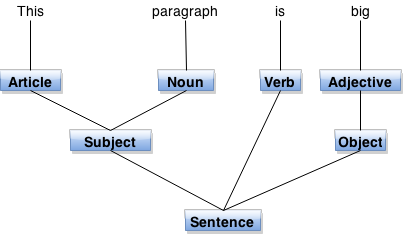
\includegraphics[width=0.7\textwidth]{img/parsing.png}
%\end{center}
%\caption{Parsing}
%\label{fig:parsing}
%\end{figure}

%\newpage

Once the sentence structure is understood, we must extract the "meaning" with the semantic analyzer.
The duty of the semantic analyzer is to perform some contextual checks to catch language inconsistencies and build an intermediate representation to store the meaning of the source text.
After that, it may or may not have some optimization regarding the source code.  

Finally, the code generator translates the intermediate representation of the high-level programming into assembly code (lower level programming).
At this stage, a new optimization phase can occur to deliver an object code shorter and faster than the original one.

Notice that the task of constructing a compiler for a particular source language is complex. 
To simplify this task, it is usual to resort to a compiler generator that is a system able to build automatically a language processor from the language grammar.
In this master project, the compiler generator ANTLR was used, as we will be described in section~\ref{sct:compiler_generation_with_antlr}.

The first tool steps, lexical and syntatical analysis, will be briefly discussed in section~\ref{sct:lexical_and_syntatical_analysis}. Then section~\ref{sct:semantic_analysis} explains in detail the implementation of LISS semantic analyzer.
To conclude the chapter, section~\ref{sct:code_generation} provides also details about the implementation of the LISS code generator.

%\newpage



%%%%%%%%%%%%%%%%%%%%%%%%%%%

%\section{Summary}
%\section{ANTLR}
\section{Compiler generation with ANTLR}
\label{sct:compiler_generation_with_antlr}

Terence Parr, the man who is behind ANTLR (ANother Tool for Language Recognition ~\citep{parr2007,Par05}) made a parser (or more precisely, a compiler) generator that reads a context free grammar, a translation grammar, or an attribute grammar and produces automatically a processor (based on a LL(k) recursive-descent parser) for the language defined by the input grammar.

An ANTLR specification is composed by two parts : the one with all the grammar rules and the other one with lexer grammar.

Listing ~\ref{lst:agANTLR} is the one with the grammar rules; in that case it is an  example of an AG (Attribute Grammar).

\begin{comment}
\begin{figure}[h!]
  \centering
    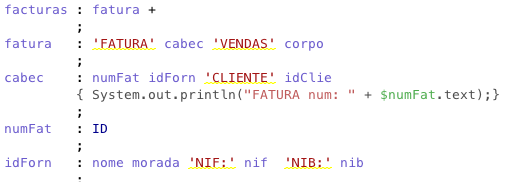
\includegraphics[width=0.8\textwidth]{img/gaAnTLR.png}
    \caption{GA representation on ANTLR}
    \label{fig:gaAntlr}
\end{figure}
\end{comment}

\begin{lstlisting}[caption={AG representation on ANTLR},label={lst:agANTLR}]
facturas : fatura +
         ;
fatura   : 'FATURA' cabec 'VENDAS' corpo
         ;
cabec    : numFat idForn 'CLIENTE' idClie
         { System.out.println("FATURA num: " + $numFat.text);}
         ;
numFat   : ID
         ;
idForn   : nome morada 'NIF:' nif  'NIB:' nib
\end{lstlisting}


On the other hand, the lexer grammar defines the lexical rules which are regular expressions as can be seen in Listing ~\ref{lst:lexer}. They define the set of possible character sequences that are used to form individual tokens. A lexer recognizes strings and for each string found, it produces the respective tokens. %(see figure~\ref{lst:lexer}).

\begin{comment}
\begin{figure}[h!]
  \centering
    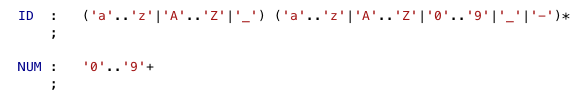
\includegraphics[width=0.8\textwidth]{img/lexer.png}
    \caption{Lexer representation}
    \label{fig:lexer}
\end{figure}
\end{comment}

\begin{lstlisting}[caption={Lexer representation},label={lst:lexer}]
/*--------------- Lexer ---------------------------------------*/

ID  :   ('a'..'z'|'A'..'Z'|'_') ('a'..'z'|'A'..'Z'|'0'..'9'|'_'|'-')*
    ;

NUM :   '0'..'9'+
\end{lstlisting}



%\newpage
\section{Lexical and syntatical analysis}
\label{sct:lexical_and_syntatical_analysis}

The parser generator by ANTLR will be able to create an abstract syntax tree (AST) which is a tree representation of the abstract syntactic structure of source code written in a programming language (see Figure~\ref{fig:AST}).

\begin{figure}[h!]
  \centering
    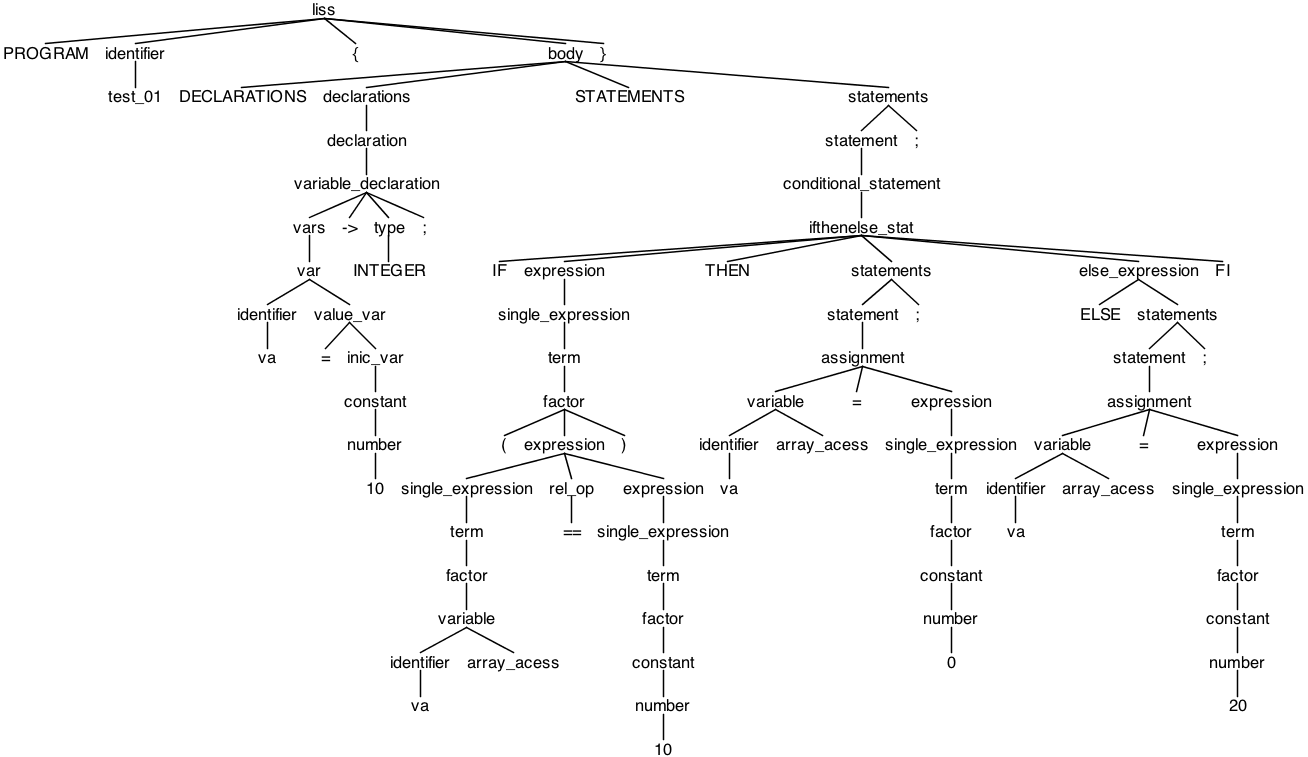
\includegraphics[width=1\textwidth]{img/antlr4_parse_tree.png}
    \caption{AST representation}
    \label{fig:AST}
\end{figure}

ANTLR will be used to generate MIPS assembly code according to the semantic rule specified in the AG for LISS language.







\section{Semantic Analysis}
\label{sct:semantic_analysis}






\subsection{Symbol Table}

A symbol table is a data structure used for the compiler, which helps to store some valuable informations for identifiers in a program's source code. Basically, it helps the compiler for finding some semantic errors regarding to the translation of the program which will be done later.

There are a lot of types of data structure for creating a symbol table. From one large symbol table for all symbols or separated, hierarchical symbol tables for different scopes.

\begin{figure}[h!]
  \centering
    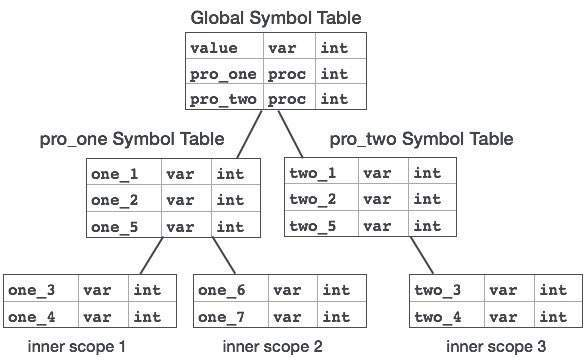
\includegraphics[width=0.8\textwidth]{img/symbol_table_hierarchical.jpg}
    \caption{Example of hierarchical symbol table}
    \label{fig:hierarchical_symbol_table}
\end{figure}

%For this project, we used one large symbol table for all symbols and we will explain in the next section.

\newpage

\subsubsection{Symbol Table in LISS}

For this project, we used a one large symbol table for all symbols.

Let's explain throw the Figure ~\ref{fig:global_symbol_table_liss} how it works the symbol table in LISS.

\begin{figure}[h!]
  \centering
    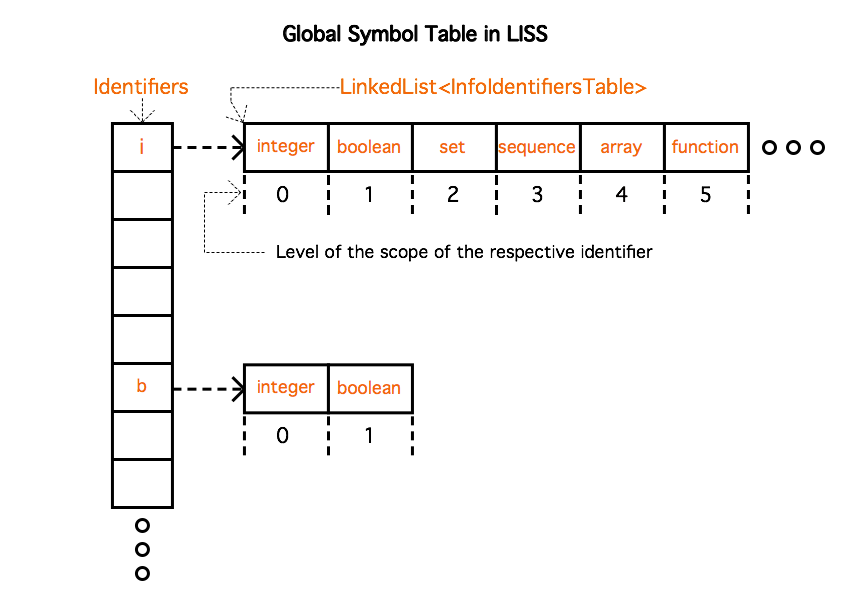
\includegraphics[width=1\textwidth]{img/global_symbol_table.png}
    \caption{Global symbol table in LISS}
    \label{fig:global_symbol_table_liss}
\end{figure}

For our project we implemented the symbol table with a HashMap where the key is an identifier and the value is a LinkedList of some informations related to the identifier.

\begin{lstlisting}[caption={Data structure of the symbol table in LISS},label={lst:symbol_table_liss_java_implementation}]
	HashMap<String, LinkedList<InfoIdentifiersTable>>
\end{lstlisting}

The identifier (related to ~\textit{String} word in ~\ref{lst:symbol_table_liss_java_implementation}) must be unique (concept of using a HashMap) and the ~\textit{LinkedList} must have the idea of an ordered list.
%, that's why we choosed to use a ~\textit{HashMap} data structure associated to a ~\textit{LinkedList}.

Basically, the identifier is associated to a ~\textit{LinkedList} of informations related to the identifier and those informations explain which category and type is the identifier.

For our project, we have 3 different categories:
\begin{enumerate}
\item TYPE
\item VAR
\item FUNCTION
\end{enumerate}

\subsubsection{TYPE category}

The ~\textit{TYPE} category contains informations about which primative type is available in LISS. In our cases, they are known by : set, integer, sequence and boolean. 
It contains information about their fixed size of each type in MIPS as well as their level scope.

\begin{table}[h!]
\centering
\caption{TYPE category information}
\label{tbl:type_category_information}
\begin{tabular}{l|c|c|c}
\multicolumn{1}{c|}{Identifier} & \multicolumn{1}{l|}{Category} & \multicolumn{1}{l|}{Level} & \multicolumn{1}{l}{Space (Bytes)} \\ \hline
set                             & TYPE                          & 0                          & 0                                 \\ \hline
integer                         & TYPE                          & 0                          & 4                                 \\ \hline
boolean                         & TYPE                          & 0                          & 4                                 \\ \hline
sequence                        & TYPE                          & 0                          & 4                                
\end{tabular}
\end{table}

\subsubsection{VAR category}

The ~\textit{VAR} category contains informations about the variables declared in LISS code (under ~\textit{declarations} part). It might be an integer, boolean, array, set or a sequence variable.
And each variable have different respective informations for their type associated.

Let's see and explain each type.

\begin{table}[h!]
\centering
\caption{Information related for an integer variable}
\label{tbl:var_integer_information}
\begin{tabular}{l|c|c|c|c}
\multicolumn{1}{c|}{Identifier} & Category & Level & Type    & Address \\ \hline
int                             & VAR      & 0     & integer & 0      
\end{tabular}
\end{table}

In Table ~\ref{tbl:var_integer_information}, we can see the type of information that an integer variable stores into the symbol table:
\begin{itemize}
\item ~\textit{Identifier} - name of the variable.
\item ~\textit{Category} - the category of the identifier: variable.
\item ~\textit{Level} - the level scope of the variable.
\item ~\textit{Type} - the type of the variable (integer).
\item ~\textit{Address} - the address of the variable in the stack memory.
\end{itemize}

\newpage

\begin{table}[h!]
\centering
\caption{Information related for a boolean variable}
\label{tbl:var_boolean_information}
\begin{tabular}{l|c|c|c|c}
\multicolumn{1}{c|}{Identifier} & Category & Level & Type    & Address \\ \hline
bool                            & VAR      & 1     & boolean & 4      
\end{tabular}
\end{table}

In Table ~\ref{tbl:var_boolean_information}, this is the type of information that a boolean variable stores in the symbol table.

\begin{itemize}
\item ~\textit{Identifier} - name of the variable.
\item ~\textit{Category} - the category of the identifier: variable.
\item ~\textit{Level} - the level scope of the variable.
\item ~\textit{Type} - the type of the variable (boolean).
\item ~\textit{Address} - the address of the variable in the stack memory.
\end{itemize}

\begin{table}[h!]
\centering
\caption{Information related to an array variable}
\label{tbl:var_array_information}
\begin{tabular}{l|c|c|c|c|l|l}
\multicolumn{1}{c|}{Identifier} & Category & Level & Type    & Address & Dimension              & Limits                        \\ \hline
array\_1                        & VAR      & 0     & array & 8       & \multicolumn{1}{c|}{2} & \multicolumn{1}{c}{{[}2$|$3{]}}
\end{tabular}
\end{table}

In Table ~\ref{tbl:var_array_information}, this is the type of information related to an array.
\begin{itemize}
\item ~\textit{Identifier} - name of the variable.
\item ~\textit{Category} - the category of the identifier: variable.
\item ~\textit{Level} - the level scope of the variable.
\item ~\textit{Type} - the type of the variable (array).
\item ~\textit{Address} - the address of the variable in the stack memory.
\item ~\textit{Dimension} - the number of dimension for the array.
\item ~\textit{Limits} - the limits of each dimension of the array.
\end{itemize}

\begin{table}[h!]
\centering
\caption{Information related to a set variable}
\label{tbl:var_set_information}
\begin{tabular}{l|c|c|c|c|l}
\multicolumn{1}{c|}{Identifier} & Category & Level & Type    & Address & Tree Allocated              \\ \hline
set\_1                          & VAR      & 0     & set & NULL     & \multicolumn{1}{c}{{[}x{]}}
\end{tabular}
\end{table}

In Table ~\ref{tbl:var_set_information}, this is the type of information for a set.
\begin{itemize}
\item ~\textit{Identifier} - name of the variable.
\item ~\textit{Category} - the category of the identifier: variable.
\item ~\textit{Level} - the level scope of the variable.
\item ~\textit{Type} - the type of the variable (set).
\item ~\textit{Address} - address in the stack memory, but sets doesn't need to. It creates the MIPS assembly code.
\item ~\textit{Tree Allocated} - indicates if the sets was initiated or not. If an 'X' letter appears, it means that the sets was initiated.
\end{itemize}

\begin{table}[h!]
\centering
\caption{Information related to a sequence variable}
\label{tbl:var_sequence_information}
\begin{tabular}{l|c|c|c|c|l}
\multicolumn{1}{c|}{Identifier} & Category & Level & Type     & Address & Elements\_type              \\ \hline
sequence\_1                     & VAR      & 0     & sequence & 32      & \multicolumn{1}{c}{integer}
\end{tabular}
\end{table}

In Table ~\ref{tbl:var_sequence_information}, this is the type of information for a set.
\begin{itemize}
\item ~\textit{Identifier} - name of the variable.
\item ~\textit{Category} - the category of the identifier: variable.
\item ~\textit{Level} - the level scope of the variable.
\item ~\textit{Type} - the type of the variable (sequence).
\item ~\textit{Address} - address in the stack memory.
\item ~\textit{Elements\_type} - indicates the type of the elements.
\end{itemize}

\subsubsection{FUNCTION category}

Lastly, the ~\textit{FUNCTION} category contains informations about the subprograms created in a LISS code.

\begin{table}[h!]
\centering
\caption{Information related to a function}
\label{tbl:function_information}
\begin{tabular}{l|c|c|c|c|c|c}
\multicolumn{1}{c|}{Identifier} & Category & Level & Type & Address & Nº Arguments & Type List Arguments    \\ \hline
calculate                       & FUNCTION & 0     & NULL & 32      & 2            & {[}integer, boolean{]}
\end{tabular}
\end{table}

In Table ~\ref{tbl:function_information}, this is the type of information for a function.
\begin{itemize}
\item ~\textit{Identifier} - name of the variable.
\item ~\textit{Category} - the category of the identifier: function
\item ~\textit{Level} - the level scope of the function.
\item ~\textit{Type} - the type of the function which is NULL.
\item ~\textit{Address} - size of the function stack in the stack memory (contains the list arguments, the variables declared in the subprogram and the return address of the function).
\item ~\textit{Nº Arguments} - indicates how many arguments the function does have.
\item ~\textit{Type List Arguments} - indicates the types of each arguments of the function.
\end{itemize}




Let's see the abstract data structure of InfoIdentifiersTable implemented in Figure ~\ref{fig:infoidentifierstable_structure}.

\begin{figure}[h!]
  \centering
    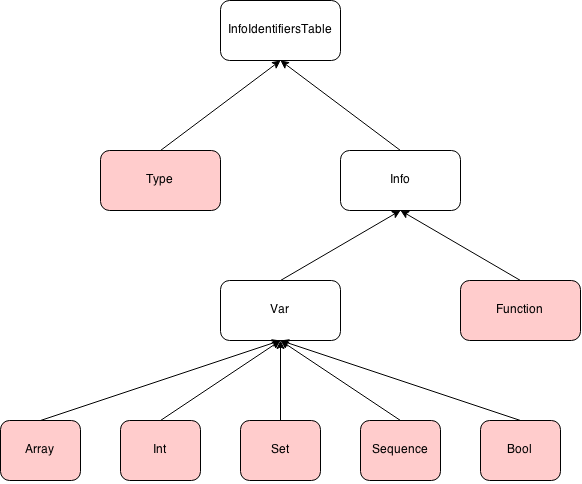
\includegraphics[width=0.8\textwidth]{img/InfoIdentifiersTable.png}
    \caption{InfoIdentifiersTable structure}
    \label{fig:infoidentifierstable_structure}
\end{figure}

Each time that an identifier is inserted into the HashMap, it inserts the information related to that identifier and in this case, the type of the identifier.
For example, in Figure ~\ref{fig:infoidentifierstable_structure} the info that will be stored in the symbol table are the red boxes.

Care that ~\textit{LinkedList} has the notion of being an ordered list, and this is a very important idea for the symbol table due to the fact that it reveals the level of the scope for the given identifier found.

In Figure ~\ref{fig:global_symbol_table_liss}, the identifier ~\textbf{b} was found in two differents level scope.
\begin{itemize}
\item Scope level 0 - Identifier ~\textbf{b} found with type ~\textit{integer}
\item Scope level 1 - Identifier ~\textbf{b} found with type ~\textit{boolean}
\end{itemize}

Notice that every time, we look for an identifier and his respective info in the symbol table. It will always take the latest info in the ~\textit{LinkedList} data structure. 

In the case of the identifier example ~\textbf{b} in Figure ~\ref{fig:global_symbol_table_liss}, it will be the ~\textbf{boolean} info.



Also, every time that a function ( ~\textit{subprogram} in LISS) is exited, we remove every information  available to the respective level scope of the function in the symbol table. And this is due for having a good consistency regarding to the information available in the symbol table.

Let's see the functions created and available in the project, regarding to the symbol table structure in JAVA.

\begin{itemize}
\item getSymbolTable - gets the symbol table.
\item doesExist - checks if a certain identifier is available.
\item getInfoIdentifier - gets the latest information of a certain identifier.
\item removeLevel - removes every information according to the level scope of every identifier available in the symbol table.
\item getAddress - gets the latest address (this address is related to the next position of an identifier that will be added in the symbol table).
\item setAddress - sets a new address.
\item add - adds identifiers into the symbol table.
\item toString - gets the representation of the symbol table as a string.
\end{itemize}

\subsection{Semantic system}

In programming language theory, the word ~\textit{semantics} is concerned by the field of studying the meaning of programming languages.
And in this field, it concerns about a lot of area.
For our project, every time that we see an inconsistency, we report them to an error table.
Let's see which kind of inconsistency we can find for our project.

\begin{enumerate}
\item Finding inconsistency in types and their related specifications.
\item Finding inconsistency in variables declared or not.
\item Finding inconsistency regarding to the use of multiple expressions.
\item Finding inconsistency for returning types of functions created.
\end{enumerate}

This will be talked later, let's understand firstly the error table system created.

\subsection{Error table in LISS}

The error table let the user to understand the problems that he is having with the code when he is trying to create or making it.
In this way, it will facilitate the user to correct the problems found regarding to his code with ease.

Let's see the table error structure made for our project in Figure ~\ref{fig:error_table_structure}.

\begin{figure}[h!]
  \centering
   % 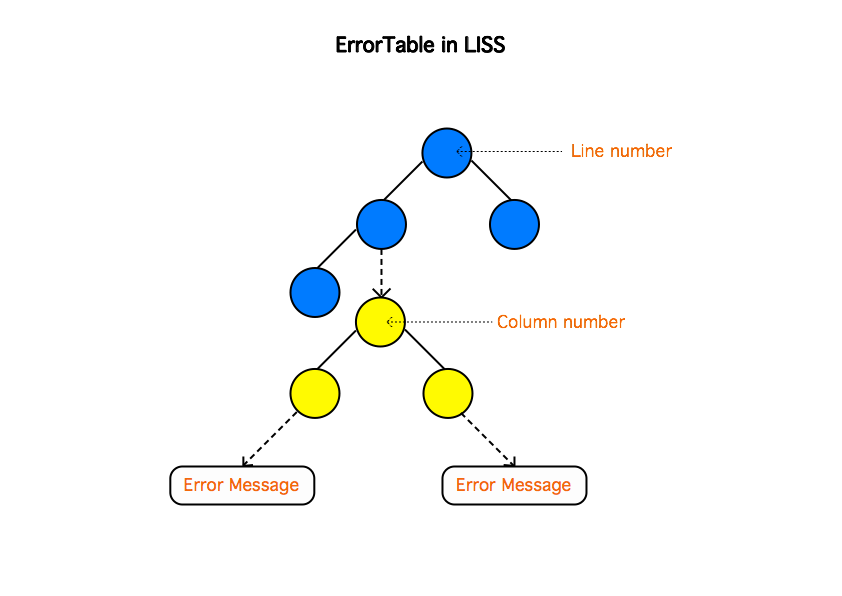
\includegraphics[width=0.8\textwidth]{img/errorTable.png}
    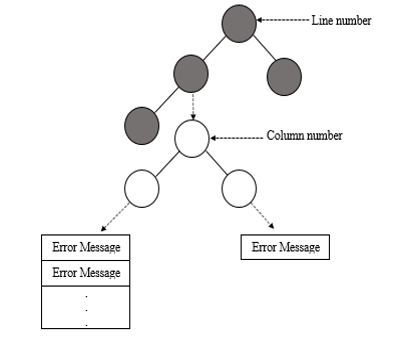
\includegraphics[width=0.9\textwidth]{img/error_table_liss.png}
    \caption{ErrorTable structure}
    \label{fig:error_table_structure}
\end{figure}

For our project, we managed to create a data structure which could handle some error messages and could give us also some informations related to the error message (line and column number).

And this was done by creating that data structure in JAVA:

\begin{lstlisting}[caption={Data structure of the error table in LISS},label={lst:error_table_liss_java_implementation}]
	TreeMap<Integer,TreeMap<Integer,ArrayList<String>>>
\end{lstlisting}

Basically, this data structure is divided into two ~\textit{TreeMap} (those ~\textit{TreeMap} can be seen in Figure ~\ref{fig:error_table_structure}, black and white) and a list (~\textit{ArrayList} data structure) of some error messages.

We choosed the ~\textit{TreeMap} data structure for one reason, the map is sorted according to the natural ordering of its keys.
This means that each time we insert in the ~\textit{TreeMap} data structure, the information is ordered by his key beside that also the key will be unique.
In this case, the first ~\textit{TreeMap} is concerned for ordering the line number of the error message (black tree in Figure ~\ref{fig:error_table_structure}).

Then when the line number is added and ordered, we add some information linked to the line number and this is the column number of the line (white tree in Figure ~\ref{fig:error_table_structure}).

Finally, we add the error messages to the list related to a certain line and column.

With that data structure, we are sure that it can have a list of error messages for a certain line and column numbers and that the line and the column number are ordered for an ease interpretation for the user in solving the problem regarding to his code.

%example of an error message
Let's see an example of the error table in Figure ~\ref{lst:error_table_liss_java_example}.

%This error table was thrown by the example Errors.liss
\begin{lstlisting}[caption={Example of an error table},label={lst:error_table_liss_java_example}]
	ERROR TABLE:
	  line: 5:18	Expression 'b'  has type 'boolean',when It should be 'integer'.
	  line: 6:11	Expression 'flag'  has type 'integer',when It should be 'boolean'.
	  line: 7:1	Expression 'array1=[[1,2],[2,3,4,5]],vector' has a problem with his limits.
	  line: 8:1	Expression 'vector' already exists.
	  line: 10:4	Expression 'seq1' already exists.
	  line: 14:4	Expression 'b' already exists.
\end{lstlisting}

\subsection{Types of error message}

For our error table structure, we needed to add some informations relatively to the error message thrown.
And as we said, previously, we have different kind of types for some error messages.

Let's see in the Table ~\ref{tbl:types_error_message}.

\newpage

\begin{table}[h!]
\centering
\caption{Types of error message in LISS}
\label{tbl:types_error_message}
\begin{tabular}{|c|l|}
\hline
\textbf{Error type number} & \multicolumn{1}{c|}{\textbf{Error message}}                                                                                                                                                                                                                                                                                                                                             \\ \hline
1                          & Variable \textless name\_of\_variable \textgreater isn't declared                                                                                                                                                                                                                                                                                                                       \\ \hline
2                          & Variable \textless name\_of\_the\_variable \textgreater already exists.                                                                                                                                                                                                                                                                                                                 \\ \hline
3                          & Variable \textless name\_of\_the\_array\_variable \textgreater must be an 'array'.                                                                                                                                                                                                                                                                                                      \\ \hline
4                          & Variable \textless name\_of\_the\_array\_variable \textgreater has a problem with his limits.                                                                                                                                                                                                                                                                                           \\ \hline
5                          & \begin{tabular}[c]{@{}l@{}}Variable \textless name\_of\_the\_variable \textgreater has type \textless type\_found \textgreater, when it\\  should be \textless type\_expected \textgreater.\end{tabular}                                                                                                                                                                                \\ \hline
6                          & Incompatible types in Assignment.                                                                                                                                                                                                                                                                                                                                                       \\ \hline
7                          & \begin{tabular}[c]{@{}l@{}}Expression \textless expression\_string \textgreater has type \textless type\_found \textgreater, when it \\ should be \textless type\_expected \textgreater.\end{tabular}                                                                                                                                                                                   \\ \hline
8                          & \begin{tabular}[c]{@{}l@{}}Function \textless name\_of\_the\_function \textgreater has return type \textless type\_found \textgreater, \\ when it should be \textless type\_expected \textgreater.\end{tabular}                                                                                                                                                                         \\ \hline
9                         & Variable \textless name\_of\_the\_function \textgreater is not a function.
 \\ \hline
10                        & \begin{tabular}[c]{@{}l@{}}Expression \textless expression\_string \textgreater has type \textless left\_type\_found \textgreater \\ \textless operator\_string \textgreater \textless right\_type\_found \textgreater, required type \\ \textless left\_type\_required \textgreater \textless operator\_string \textgreater \textless right\_type\_required \textgreater.\end{tabular} \\ \hline
11                         & \begin{tabular}[c]{@{}l@{}}Expression \textless name\_of\_the\_array\_variable \textgreater has dimension \\ \textless dimension\_found \textgreater, when it should be equal to \\ \textless dimension\_required \textgreater.\end{tabular}                                                                                                                                            \\ \hline
12                         & 'stepUp' or 'stepDown' expression, not valid with "inArray" operation.                                                                                                                                                                                                                                                                                                                      \\ \hline
13                         & 'satisfying' expression, not valid with "inArray" operation.                                                                                                                                                                                                                                                                                                                              \\ \hline
14                         & Function \textless name\_of\_the\_function \textgreater does not exist.                                                                                                                                                                                                                                                                                                                 \\ \hline
15                         & \begin{tabular}[c]{@{}l@{}}Expression \textless name\_of\_the\_array\_variable \textgreater doesn't have the same \\ limits or dimensions.\end{tabular}                                                                                                                                                                                                                                 \\ \hline
\end{tabular}
\end{table}

Notice that in Table ~\ref{tbl:types_error_message}, we have every messages used and thrown (when necessary) for the compiler and some of them have a certain semantic structure which we need to explain.
For example, every marks:
\begin{lstlisting}
	<...>
\end{lstlisting}
found in the table message, means that it must be replaced by the correct name according to the environment that the error was found.

Let's see an example in Listing ~\ref{lst:error_liss_example} to understand better the usage of the mark.
\begin{lstlisting}[label={lst:error_liss_example},caption={Partial Listing}]
program Errors{
	declarations
		seq1 =<<1,2,3,4>> -> sequence;
		seq1 = <<1,4,7>> -> sequence;
	statements
}
\end{lstlisting}

In Listing ~\ref{lst:error_liss_example}, we have a LISS program which has two variables with the same name in the declarations part. As all programming language have, this behaviour of declaring two variables in the same level scope is prohibited, so the compiler must throw an error.

Let's see the error table in Listing ~\ref{lst:error_table_example_liss}.

\begin{lstlisting}[label={lst:error_table_example_liss},caption={Error table related to Listing ~\ref{lst:error_liss_example}}]
  ERROR TABLE:
  line: 4:2	Variable 'seq1' already exists.
\end{lstlisting}

The error table in ~\ref{lst:error_table_example_liss}, has an error message with the number 2 message type (see Table ~\ref{tbl:types_error_message}).
And we can see that the mark was replaced by the name of the variable (as said in the Table ~\ref{tbl:types_error_message} regarding to the message number 2 type).
And this is the same behavior regarding to the others messages available in the Table ~\ref{tbl:types_error_message}.

Now, let's explain the Table ~\ref{tbl:types_error_message} for an ease interpretation of those messages.

\begin{enumerate}
\item Message for variable that are not declared.
\item Message for variables that already exists.
\item Message for variables that must be an array and they are not.
\item Message for variables that are an array type and their limits doesn't match.
\item Message for variables that have a certain type, but they should have another type. 
\item Message regarding to different types when an assignment is found. For example : 'integer' = 'boolean'. 
\item Message for expressions that has different types.
\item Message for functions regarding to the return type which might be different.
\item Message for functions which the name of the function doesn't have the type function and does have another type.
\item Message for expressions which has different types according to the operator who is being used. For example: 'integer' + 'boolean'. 
\item Message for arrays that has different dimension, according to his declaration.
\item Message for unconditional loop that use 'stepUp' or 'stepDown' expression.
\item Message for unconditional loop that use 'satisfying' expression.
\item Message for functions where the name of the function doesn't exist.
\item Message for arrays where the limits or the dimension isn't equal as the declared array variable.
\end{enumerate}


\subsection{Usage of error messages}

In this section, we are going to report where the error message will be thrown in the compiler regarding to the attribute grammar that we have.

\subsubsection{Variable declaration}

\begin{lstlisting}[label={lst:variable_declaration_error},caption={Variable declaration rule in LISS}]
  variable_declaration : vars '->' type ';'
\end{lstlisting}

In Listing ~\ref{lst:variable_declaration_error}, this is the part where we declare some variables with the types chosen under the declarations part.
And this also where we add the information into the symbol table too.
So, before we add the information into the symbol table, we need to check if every variables does have the correct type regarding to the type chosen. If not, then it will throw the number 5 error message (see Table ~\ref{tbl:types_error_message}).

Let's see an error that might happen for this case in Listing ~\ref{lst:example_error_message_variable_declaration}.

\begin{lstlisting}[label={lst:example_error_message_variable_declaration},caption={Example of an error message in variable declaration}]
  b = boolean -> integer;
\end{lstlisting}

Notice that in this section, we create the mips code for every variables. And there is one type which can throw an error message too in this section, it is called the ~\textit{array} type. For this type, we need to check if the limits are correct, if they are not then it throw the number 4 error message (see Table ~\ref{tbl:types_error_message}).

Regarding to the others type, we don't check in this section. Because the ~\textit{array} type, is the only one who is the hardest one to deal (needs to calculate the position of the array) for creating the mips code instruction.

Let's see an example of an array type error message regarding to this case in Listing ~\ref{lst:example_error_message_variable_declaration_2}.

\begin{lstlisting}[label={lst:example_error_message_variable_declaration_2},caption={Example of an error message in variable declaration for the array type}]
  array1 = [[1,2],[2,3,4,5]], vector -> array size 4,3;
\end{lstlisting}

\subsubsection{Vars}

\begin{lstlisting}[label={lst:vars_error_message},caption={Vars rule in LISS}]
  vars : v1 (',' v2)*
\end{lstlisting}

In Listing ~\ref{lst:vars_error_message}, this grammar part refers to the declaration of multiple variables in a same line under the declarations section in LISS.

And for this part we need to check if the variables that will be added to the symbol table, they are already created or not. If they are already, then the number 2 error message will be thrown (see Table ~\ref{tbl:types_error_message}).
Let's see an example of LISS that can throw this error in the error table in Listing ~\ref{lst:example_var_error_message_liss}.

\begin{lstlisting}[label={lst:example_var_error_message_liss},caption={Example of an error message in LISS for vars non-terminal}]
  a = 4, a = 5 -> integer;
\end{lstlisting}

In Listing ~\ref{lst:example_var_error_message_liss}, there is a problem regarding that two variables with the same name are being created. This must throw an error as we said previously, and an error message related to the second variable.

\subsubsection{Set initialization}

\begin{lstlisting}[label={lst:set_initialization_error_message},caption={Set initialization rule in LISS}]
  set_initialization :                    
                     | identifier '|' expression
\end{lstlisting}

In Listing ~\ref{lst:set_initialization_error_message}, this part refers for declaring a set under the declarations section in LISS.
And it has two choices for declaring a set: empty set or some content for the set.
If there is some content available, this content must be a boolean expression. In case the expression isn't a boolean, it will throw an error message to the error table and this will be the number 7 error message (see Table ~\ref{tbl:types_error_message}).
Let's see an example of  this error with a piece of LISS code related to set initialization in Listing ~\ref{lst:example_set_initialization_error_message}.

\begin{lstlisting}[label={lst:example_set_initialization_error_message},caption={Example of an error message in LISS for set\_initialization non-terminal}]
  set6 = { z | (z+tail(z)) < 5} -> set;
\end{lstlisting}

In Listing ~\ref{lst:example_set_initialization_error_message}, we can see that the variable won't be declared due to the fact that the content isn't correct. The function ~\textit{tail} is a function for sequence and it needs a sequence variable as an argument, not an integer variable (as we can see). The compiler will return the type of that operation as 'null' because he can't execute that operation.

Then, there is an sum operator who needs a variable of type integer. But due to the previous statements we have made, the type that the sum operator will have, are: integer (from ~\textit{z} variable) and a null (from ~\textit{tail(z)}). 
The compiler can't execute it too, so the error is being spread throw the entire operation of the set content.

In the end, after calculating the content of the set initialization of the set, the error table will have that comment regarding to that variable in Listing ~\ref{lst:error_message_set_initialization}.

\begin{lstlisting}[label={lst:error_message_set_initialization},caption={Error message for the set\_initialization}]
  line: 20:18	Expression '(z+tail(z))<5'  has type 'null',when It should be 'boolean'.
\end{lstlisting}

\subsubsection{Subprogram definition}

\begin{lstlisting}[label={lst:subprogram_definition_error_message},caption={Subprogram definition rule in LISS}]
  subprogram_definition : 'subprogram' identifier '('  formal_args ')' return_type f_body
\end{lstlisting}

In Listing ~\ref{lst:subprogram_definition_error_message}, this part refers for declaring any subprogram (functions) under the declaration section in LISS.
And for this part we need to check the return type of the subprogram.

If the return type has a different type chosen and type needed (for example, type chosen is boolean, but the return type is an integer) then the number 7 error message (see Table ~\ref{tbl:types_error_message}) is thrown.

Let's see an example of this case in Listing ~\ref{lst:error_message_subprogram_definition}.

\begin{lstlisting}[label={lst:error_message_subprogram_definition},caption={Example of error message in LISS for subprogram\_definition non\_terminal}]
  subprogram f(amen->boolean)->integer{
        declarations
               b -> boolean;
        statements
        return b;
  }
\end{lstlisting}

In Listing ~\ref{lst:error_message_subprogram_definition}, we can see that the return type permitted is an integer. But with this example, the subprogram returns a variable called 'b' and has a boolean type. In this case, an error message will be reported due to the incorrectness type.

\subsubsection{Assignment}

\begin{lstlisting}[label={lst:assignment_error_message},caption={Assignment rule in LISS}]
  assignment : designator '=' expression
\end{lstlisting}

In Listing ~\ref{lst:assignment_error_message}, this part refers for assigning some content to a variable or an array under the statement section in LISS.
And for this part we need to check some error messages regarding to the context available.
Let's explain those differents context below.

If the designator non-terminal in Listing ~\ref{lst:assignment_error_message}, is a variable of type ~\textit{array}. It means that we can store some content for that variable (see example of this case in Listing ~\ref{lst:store_values_to_array_assignment}).

\begin{lstlisting}[caption={Example of storing some values to an array variable},label={lst:store_values_to_array_assignment}]
  array1 = [1,2,3];
\end{lstlisting}

In Listing ~\ref{lst:store_values_to_array_assignment}, we see a variable named ~\textit{array1} with the type ~\textit{array} and it will be assigned to some values shown in the example, ~\textit{[1,2,3]}. For this example, we need to check if the values have the correct dimension and limits regarding the variable. In this case, if it isn't correct then the number 15 error message ( see Table ~\ref{tbl:types_error_message}).

Also the same error message is reported for the case of the next example in Listing ~\ref{lst:storing_one_value_to_an_array_assignment}.

\begin{lstlisting}[caption={Example of storing a value to a certain position in the array},label={lst:storing_one_value_to_an_array_assignment}]
  array[3] = 1;
\end{lstlisting}

In Listing ~\ref{lst:storing_one_value_to_an_array_assignment}, if the variable ~\textit{array} has only two position available. This means that the access of the fourth position (as shown in the example), it is behind of the limits regarding to the specification of the variable.
And, in this case, it must throw the number 15 error message too ( see Table ~\ref{tbl:types_error_message}).

Last case for this part concerns about the types of ~\textit{designator} non-terminal and ~\textit{expression} non-terminal not being equals. In this case, the compiler can't execute and procede with the assignment operation.

This will throw the number 6 error message to the error table (see Table ~\ref{tbl:types_error_message}).

Let's see an example of this case in Listing ~\ref{lst:different_types_assignment}.

\begin{lstlisting}[caption={Example of assignment with differents types},label={lst:different_types_assignment}]
  boolean1 = integer1;
\end{lstlisting}

In Listing ~\ref{lst:different_types_assignment}, the example informs us that assignment operation is trying to store an integer to the ~\textit{boolean1} variable (which has the boolean type).
As we know, if the types aren't equals then the operations cannot be executed and must report an error.

\subsubsection{Designator}

\begin{lstlisting}[caption={Designator rule in LISS},label={lst:designator_error_message}]
  designator : identifier array_access
\end{lstlisting}

In Listing ~\ref{lst:designator_error_message}, this part refers for using a variable or an array variable under the statement section in LISS.
And we need to check some errors when it used only for a variable context or in the array variable context.

Let's speak firstly for the variable context.

If it is only the variable context, the ~\textit{array\_access} is not available but, only, the ~\textit{identifier} non-terminal will be available.

Every variable used must be declared in the symbol table. If it doesn't exist in the symbol table, it means that variable doesn't exist and we need to throw an error in the error table, number 1 error message (see Table ~\ref{tbl:types_error_message}).

We need to check if the name of the ~\textit{identifier} isn't the same as the name of a type in LISS (see Table ~\ref{tbl:type_category_information}). If it is, then it must throw the number 1 error message to the error table (see Table ~\ref{tbl:types_error_message}).

Now regarding to the array variable context, we need to check a lot of errors.

Firstly, we need to check if the identifier is available in the symbol table otherwise it will throw the number 1 error message to the error table (see Table ~\ref{tbl:types_error_message}).
 
Secondly, we need to check if the name of the identifier isn't the same name as the name of a type in LISS (see Table ~\ref{tbl:type_category_information}). If it is, then it must throw the number 1 error message to the error table (see Table ~\ref{tbl:types_error_message}).

Thirdly, we need to check the type of identifier. If the type isn't an array then we need to throw the number 3 error message (see Table ~\ref{tbl:types_error_message}).

And finally, we need to check if the ~\textit{identifier} and the ~\textit{array\_access} non-terminal have the same dimension. If they don't have then it must be throw the number 11 error message to the error table (see Table ~\ref{tbl:types_error_message}).

\subsubsection{Elem array}

\begin{lstlisting}[caption={Elem\_array rule in LISS},label={lst:elem_array_error_message}]
  elem_array : s1=single_expression ( ',' s2=single_expression )*
\end{lstlisting}

In Listing ~\ref{lst:elem_array_error_message}, this part refers to the elements of an array.
And for this part we need to check if every elements (represented by the ~\textit{single\_expression} non-terminal) has the correct type.

In an array context, the type of each elements must be an integer. If it isn't then it must throw the number 7 error message to the error table (see Table ~\ref{tbl:types_error_message}).

\subsubsection{Function call}

\begin{lstlisting}[caption={Function\_call rule in LISS},label={lst:function_call_error_message}]
  function_call : i=identifier '(' sub_prg_args ')'
\end{lstlisting}

In Listing ~\ref{lst:function_call_error_message}, this part is related to call some functions under the statement section in LISS.
For this context, we need to check two things regarding to errors.

Firstly, we need to check if the ~\textit{identifier} is available in the symbol table. If it isn't then it must throw the number 14 error message to the error table (see Table ~\ref{tbl:types_error_message}).

Lastly, we need to check if the ~\textit{identifier} has the correct type ( ~\textit{Function} type). If it doesn't have then it must throw the number 9 error message to the error table (see Table ~\ref{tbl:types_error_message}).

\subsubsection{Expression}

\begin{lstlisting}[caption={Expression rule in LISS}, label={lst:expression_error_message}]
  expression : single_expression (rel_op single_expression )?
\end{lstlisting}

In Listing ~\ref{lst:expression_error_message}, this part refers to expression that can be used in a various way in LISS. 
For this case, we need to check if the type of both ~\textit{single\_expression} non-terminal are correct in relation to the type required for the ~\textit{rel\_op} non-terminal. If they are not, then we throw the number 10 error message to the error table (see Table ~\ref{tbl:types_error_message}). 

Notice that it is the ~\textit{rel\_op} non-terminal who tells which type that the left and right ~\textit{single\_expression} non-terminal must have.

Let's see an example in Listing ~\ref{lst:example_expression_error_message}.

\begin{lstlisting}[caption={Example of an error message in expression rule},label={lst:example_expression_error_message}]
  2 < true
\end{lstlisting}

In Listing ~\ref{lst:example_expression_error_message}, we can see the number two ( first single\_expression annotation ) then the minus sign (the rel\_op annotation ) and finaly the true value ( the last single\_expression annotation).
If we procede to calculate the entire expression, we can see that the types doesn't match at all between them.
In that case the minus sign needs an integer in both side (left and right), and actually it does have an integer and a boolean expression which is an error to be thrown in the error table.

\subsubsection{Single expression}

\begin{lstlisting}[caption={Single\_expresion rule in LISS},label={lst:single_expression_error_message}]
  single_expression : term ( add_op term)*
\end{lstlisting}

In Listing ~\ref{lst:single_expression_error_message}, this part refers to the expansion of the ~\textit{single\_expression} non-terminal rule of the ~\textit{expression} rule in LISS.
And the behaviour is the same as the ~\textit{expression} rule, this means that we need to check the types required for the ~\textit{add\_op} non-terminal. If ~\textit{single\_expression} non-terminal type don't coincide with the required type regarding to the ~\textit{add\_op} non-terminal, then it must throw the number 10 error message to the error table.

\subsubsection{Term}

\begin{lstlisting}[caption={Term rule in LISS},label={lst:term_error_message}]
  term : factor ( mul_op factor)*
\end{lstlisting}

In Listing ~\ref{lst:term_error_message}, this part refers to the expansion of the ~\textit{term} non-terminal rule of the ~\textit{single\_expression} rule in LISS.
And the behaviour is the same as the ~\textit{expression} rule, this means that we need to check the types required for the ~\textit{mul\_op} non-terminal. If ~\textit{factor} non-terminal type don't coincide with the required type regarding to the ~\textit{mul\_op} non-terminal, then it must throw the number 10 error message to the error table.

\subsubsection{Factor}

\begin{lstlisting}[caption={Factor rule in LISS},label={lst:factor_error_message}]
  factor : inic_var
            | designator
            | '(' expression ')'
            | '!' factor
            | function_call
            | specialFunctions
\end{lstlisting}

In Listing ~\ref{lst:factor_error_message}, this part refers to the expansion of the ~\textit{factor} non-terminal rule of the ~\textit{term} rule in LISS.
And as it can be seen, there is a lot of options for this rule.

But we will do a particular attention to a simple one choice of that rule:

\begin{lstlisting}
  '!' factor
\end{lstlisting}

Notice that there is an exclamation mark sign and then a ~\textit{factor} non-terminal. In programming langues, the exclamation mark means that it negate the expression. And this type of negation requires a boolean type in order to work correctly.
So, if the type of the ~\textit{factor} non-terminal is not a boolean. Then the number 7 error message will be added to the error table.

\subsubsection{Print\_what}

\begin{lstlisting}[caption={Print\_what rule in LISS},label={lst:print_what_error_message}]
  print_what : 
             | expression
             | string
\end{lstlisting}

In Listing ~\ref{lst:print_what_error_message}, this part refers for printing in the output with the use of LISS language.

And we need to check the type of the ~\textit{expression} non-terminal. If the type is a ~\textit{set} then it must throw the number 7 error message in the error table (see Table ~\ref{tbl:types_error_message}).

Notice that the type allowed for the ~\textit{expression} non-terminal are :

\begin{itemize}
\item integer
\item boolean
\item sequence
\item array
\end{itemize}

\subsubsection{Read}

\begin{lstlisting}[caption={Read rule in LISS},label={lst:read_error_message}]
  read_statement : 'input' '(' identifier ')'
\end{lstlisting}

In Listing ~\ref{lst:read_error_message}, this part refers for reading the input of the user which will be stored to the ~\textit{identifier} non-terminal in LISS.
And we need to check some errors for that non-terminal.

If the ~\textit{identifier} non-terminal doesn't exist in the symbol table, then we must thrown the number 1 error message (see Table ~\ref{tbl:types_error_message}).
If the ~\textit{identifier} exists in the symbol table, we must check the type of it.
If the type isn't an integer, then we must throw the number 5 error message in the error table ( see Table ~\ref{tbl:types_error_message}).

\subsubsection{If\_then\_else\_stat}

\begin{lstlisting}[caption={If\_then\_else\_stat rule in LISS},label={lst:if_then_else_stat_error_message}]
  if_then_else_stat : 'if' '(' expression ')'
                      'then' '{' statements '}'
                       else_expression
\end{lstlisting}

In Listing ~\ref{lst:if_then_else_stat_error_message}, this part refers in the use of a conditional expression and particularly, an 'if' statement.

As all programming languages, the behaviour of an 'if' statement is the same. And we do also the same in LISS, it means that the ~\textit{expression} non-terminal must be a boolean type. Because as it is a condition with an 'if' statement it will say if it will enter to that branch or to another branch regarding to the value of the condition. If the ~\textit{expression} non-terminal type isn't a boolean, then it must throw the number 7 error message to the error table ( see Table ~\ref{tbl:types_error_message}).

\subsubsection{For\_stat}

\begin{lstlisting}[caption={For\_stat rule in LISS},label={lst:for_stat_error_message}]
  for_stat : 'for' '(' interval ')' step satisfy
             {
               statements
             }
\end{lstlisting}

In Listing ~\ref{lst:for_stat_error_message}, this part refers to the use of a 'for-loop' statements in LISS.

For this particular case, we test an error regarding to the use of a 'for-each' context or not.

Remember that in LISS context, we are able to use a 'for-loop' which can access to every elements of an array, also called 'for-each'.
And with that 'for-each' context, we cannot use ~\textit{step} non-terminal and ~\textit{satisfy} non-terminal.
So we must check if we use a 'for-each' loop, if it is used then we need to check if the ~\textit{step} or ~\textit{satisfy} non-terminal are available.

If the ~\textit{step} non-terminal is available then we must throw the number 12 error message to the error table (see Table ~\ref{tbl:types_error_message}).

If the ~\textit{satisfy} non-terminal is available then we must throw the number 13 error message to the error table (see Table ~\ref{tbl:types_error_message}).

Let's see an example of those cases in Listing ~\ref{lst:for_stat_error_message_example}.

\begin{lstlisting}[caption={Example of an error message in for\_stat rule},label={lst:for_stat_error_message_example}]
  for(b inArray vector) stepDown 1 satisfying vector[0] == a
\end{lstlisting}

In Listing ~\ref{lst:for_stat_error_message_example}, the fact that there is an ~\textit{inArray} word means that the statement is a 'for-each' loop. And for this case we cannot use a ~\textit{step} or a ~\textit{satisfying} rule. But, for this case, there is.

For the compiler, it means that it must throw both the number 12 and 13 error message to the error table due to the incorectness of the language LISS.

\subsubsection{Interval}

\begin{lstlisting}[caption={Interval rule in LISS},label={lst:interval_error_message}]
  interval : identifier type_interval
\end{lstlisting}

In Listing ~\ref{lst:interval_error_message}, this part refers to the expansion of the ~\textit{interval} non-terminal rule of the ~\textit{for\_stat} rule in LISS.

We need to check if the ~\textit{identifier} non-terminal is available to the symbol table, if it isn't then it must throw the number 1 error message to the error table (see Table ~\ref{tbl:types_error_message}).

If the ~\textit{identifier} is on the symbol table, we need to check the type of the variable.

As we said before, the 'for-each' statement refers to the use of ~\textit{array}. And the type ~\textit{array}, uses only ~\textit{integer} elements. In this case, the variable ~\textit{identifier} must also have the same type, ~\textit{integer}.

So we need to check the type of the variable ~\textit{identifier} and see if it is an ~\textit{integer}.
If it isn't, then it must throw the number 5 error message to the error table (see Table ~\ref{tbl:types_error_message}).

\subsubsection{Type\_interval}

\begin{lstlisting}[caption={Type\_interval rule in LISS},label={lst:type_interval_error_message}]
  type_interval : 'in' range
                | 'inArray' identifier
\end{lstlisting}

In Listing ~\ref{lst:type_interval_error_message}, this part refers to the expansion of the ~\textit{type\_interval} non-terminal rule of the ~\textit{interval} rule in LISS. It tells us which kind of operation can be a 'for-loop' in LISS.
And as we can see there is two choices, the normal behaviour of the 'for-loop' statement (represented by ~\textit{in range}) and the 'for-each' statement (represented by ~\textit{inArray identifier}).
For this case, we make only an attention to the 'for-each' statement, and particularly to the ~\textit{identifier} terminal.

We need to check if the ~\textit{identifier} variable is on the symbol table firstly, if it isn't the number 1 error message will be throw in the error table (see Table ~\ref{tbl:types_error_message}).
Then we need to check the type that ~\textit{identifier} variable has. If the variable isn't an ~\textit{array} then it must throw the number 5 error message to the error table (see Table ~\ref{tbl:types_error_message}).

\subsubsection{Minimum}

\begin{lstlisting}[caption={Minimum rule in LISS},label={lst:minimum_error_message}]
  minimum : number
          | identifier
\end{lstlisting}

In Listing ~\ref{lst:minimum_error_message}, this part refers to the expansion of the ~~\textit{range} non-terminal rule of the ~\textit{type\_interval} rule in LISS.

For this case, we have two options; the first one is to give a number, the second one is to give a variable.
And regarding for the variable, we need to check if it is avaible in the symbol table. If it isn't then it means that it isn't declared which will be throw the number 1 error message to the error table (see Table ~\ref{tbl:types_error_message}).
But if the variable belongs to the symbol table, we need to check the type of it. If the type isn't an ~\textit{integer} then it must throw the number 5 error message to the error table (see Table ~\ref{tbl:types_error_message}).

\subsubsection{Maximum}

\begin{lstlisting}[caption={Maximum rule in LISS},label={lst:maximum_error_message}]
  maximum : number
          | identifier
\end{lstlisting}

In Listing ~\ref{lst:maximum_error_message}, this part refers to the expansion of the ~\textit{range} non-terminal rule of the ~\textit{type\_interval} rule in LISS. And the behaviour is the same as the ~\textit{minimum} rule, this means that we need to check the ~\textit{identifier} terminal (variable) in the symbol table. If it isn't available then it means that the variable isn't declared and must throw the number 1 error message to the error table (see Table ~\ref{tbl:types_error_message}).

If the variable exists, we need to check his type. If the type isn't an ~\textit{integer} then it must throw the number 5 error message to the error table (see Table ~\ref{tbl:types_error_message}).

\subsubsection{Satisfy}

\begin{lstlisting}[caption={Satisfy rule in LISS},label={lst:satisfy_error_message}]
  satisfy :
          | 'satisfying' expression
\end{lstlisting}

In Listing ~\ref{lst:satisfy_error_message}, this part refers to the expansion of the ~\textit{for\_stat} non-terminal rule of the ~\textit{satisfy} rule in LISS.
Basically, the ~\textit{satisfying} word means that there is a condition who must be calculated and should be 'true' in order to proceed.

In this case, the ~\textit{expression} is the condition and it must have a boolean type. If the ~\textit{expression} type isn't a boolean then it must throw  the number 7 error message in the error table (see Table ~\ref{tbl:types_error_message}).

\subsubsection{While\_stat}

\begin{lstlisting}[caption={While\_stat rule in LISS},label={lst:while_stat_error_message}]
  while_stat : 'while' '(' expression ')' 
               '{' statements '}'
\end{lstlisting}

In Listing ~\ref{lst:while_stat_error_message}, this part refers to the use of a condition loop and particularly named as a ~\textit{while} statement.

For this case, we need to check if the condition ( also known as ~\textit{expression} non-terminal), has the correct type.

Notice that a condition must have a ~\textit{boolean} type and we need to check if the ~\textit{expression} type is a boolean. If it isn't then it must throw the number 7 error message to the error table (see Table ~\ref{tbl:types_error_message}).

\subsubsection{Succ\_or\_pred}

\begin{lstlisting}[caption={Succ\_or\_pred rule in LISS},label={lst:succ_or_pred_error_message}]
  succ_or_pred : succ_pred identifier
\end{lstlisting}

In Listing ~\ref{lst:succ_or_pred_error_message}, this part refers for incrementing or decrementing a variable in LISS and it is used as a statement.
Regarding to this case, we need to check two things.

First, we need to check if the ~\textit{identifier} (also known as variable) is available in the symbol table. If it isn't then it must throw the number 1 error message to the error table (see Table ~\ref{tbl:types_error_message}).

In case that the variable is in the symbol table, we need to check his type associated. If the type isn't an ~\textit{integer}, then it must throw the number 5 error message to the error table (see Table ~\ref{tbl:types_error_message}).

\subsubsection{Tail}

\begin{lstlisting}[caption={Tail rule in LISS},label={lst:tail_error_message}]
  'tail' '(' expression ')'
\end{lstlisting}

In Listing ~\ref{lst:tail_error_message}, this part refers to the use of a ~\textit{sequence} function (also known by ~\textit{Tail} function).

For this case, we need to see if the ~\textit{expression} type have the correct type in order to work properly.

If the ~\textit{expression} type doesn't have the ~\textit{sequence} type, then it must throw the number 7 error message to the error table (see Table ~\ref{tbl:types_error_message}).

\subsubsection{Head}

\begin{lstlisting}[caption={Head rule in LISS},label={lst:head_error_message}]
  'head' '(' expression ')'
\end{lstlisting}

In Listing ~\ref{lst:head_error_message}, this part refers to the use of a ~\textit{sequence} function (also known by ~\textit{Head} function).

For this case, we need to see if the ~\textit{expression} type have the correct type in order to work properly.

If the ~\textit{expression} type doesn't have the ~\textit{sequence} type, then it must throw the number 7 error message to the error table (see Table ~\ref{tbl:types_error_message}).

\subsubsection{Cons}

\begin{lstlisting}[caption={Cons rule in LISS},label={lst:cons_error_message}]
  'cons' '(' expression ',' expression ')'
\end{lstlisting}

In Listing ~\ref{lst:cons_error_message}, this part refers to the use of a ~\textit{sequence} function (also known by ~\textit{Cons} function).

For this case, we need to see if both of the ~\textit{expression} non-terminal have the correct type in order to work properly.

If the first ~\textit{expression} non-terminal (the most left one) doesn't have an ~\textit{integer} type, then it must throw the number 7 error message to the error table (see Table ~\ref{tbl:types_error_message}).

Also if the second ~\textit{expression} non-terminal (the most right one) doesn't have a ~\textit{sequence} type, then it must throw the number 7 error message to the error table (see Table ~\ref{tbl:types_error_message}).

\subsubsection{Delete}

\begin{lstlisting}[caption={Delete rule in LISS},label={lst:delete_error_message}]
  delete : 'del' '(' expression ',' expression ')'
\end{lstlisting}

In Listing ~\ref{lst:delete_error_message}, this part refers to the use of a ~\textit{sequence} function (also known by ~\textit{delete} function).

For this case, we need to see if both of the ~\textit{expression} non-terminal have the correct type in order to work properly.

If the first ~\textit{expression} non-terminal (the most left one) doesn't have an ~\textit{integer} type, then it must throw the number 7 error message to the error table (see Table ~\ref{tbl:types_error_message}).

If the second ~\textit{expression} non-terminal (the most right one) doesn't have a ~\textit{sequence} type, then it must throw the number 7 error message to the error table (see Table ~\ref{tbl:types_error_message}).

\subsubsection{Copy\_statement}

\begin{lstlisting}[caption={Copy\_statement rule in LISS},label={lst:copy_statement_error_message}]
  'copy' '(' identifier ',' identifier ')'
\end{lstlisting}

In Listing ~\ref{lst:copy_statement_error_message}, this part refers to the use of a ~\textit{sequence} function (also known by ~\textit{copy} function).

For this case, we need to see if both of the ~\textit{identifier} terminal are in the symbol table and have the correct type in order to work properly.

If one of the ~\textit{identifier} aren't available in the symbol table, then it must throw the number 1 error message to the error table (see Table ~\ref{tbl:types_error_message}).

After seeing the availability of both ~\textit{identifier} in the symbol table, we need to check their type.
If both of the variables aren't a ~\textit{sequence} type, then it must throw the number 5 error message in the error table (see Table ~\ref{tbl:types_error_message}).

\subsubsection{Cat\_statement}

\begin{lstlisting}[caption={Cat\_statement rule in LISS},label={lst:cat_statement_error_message}]
  cat_statement : 'cat' '(' identifier ',' identifier ')'
\end{lstlisting}

In Listing ~\ref{lst:cat_statement_error_message}, this part refers to the use a ~\textit{sequence} function (also known by ~\textit{cat} function) and it has the same behaviour as the ~\textit{copy} statement rule. 

This means that we need to check if both of the ~\textit{identifier} terminal are in the symbol table and have the correct type in order to work properly.

If one of the ~\textit{identifier} aren't available in the symbol table, then it must throw the number 1 error message to the error table (see Table ~\ref{tbl:types_error_message}).

Then, after checking the availability of both ~\textit{identifier} in the symbol table, we need to check their type. If both of the variables aren't a ~\textit{sequence} type, then it must throw the number 5 error message in the error table (see Table ~\ref{tbl:types_error_message}).

\subsubsection{Is\_empty}

\begin{lstlisting}[caption={Is\_empty rule in LISS}, label={lst:is_empty_error_message}]
  is_empty : 'isEmpty' '(' expression ')'
\end{lstlisting}

In Listing ~\ref{lst:is_empty_error_message}, this part refers to the use of a ~\textit{sequence} function (also known by ~\textit{is\_empty} function).

For this case, we need to check, only, the type of ~\textit{expression} non-terminal.

In order to proceed the correctness of the ~\textit{is\_empty} function, the ~\textit{expression} non-terminal type must be a ~\textit{sequence}. If it isn't, then it must throw the number 7 error message to the error table (see Table ~\ref{tbl:types_error_message}).

\subsubsection{Length}

\begin{lstlisting}[caption={Length rule in LISS},label={lst:length_error_message}]
  length : 'length''(' expression ')'
\end{lstlisting}

In Listing ~\ref{lst:length_error_message}, this part refers to the use of a ~\textit{sequence} function (also known by ~\textit{length} function) and it is the same behaviour as ~\textit{is\_empty} function.

We need to check, only, the type of ~\textit{expression} non-terminal.
If the ~\textit{expression} non-terminal type isn't a ~\textit{sequence}, then it must throw the number 7 error message to the error table (see Table ~\ref{tbl:types_error_message}).

\subsubsection{Member}

\begin{lstlisting}[caption={Member rule in LISS},label={lst:member_error_message}]
  member : 'isMember''(' expression ',' identifier ')'
\end{lstlisting}

In Listing ~\ref{lst:member_error_message}, this part refers to the use of a ~\textit{sequence} function (also known by ~\textit{member} function).
For this case, we need to check firstly the ~\textit{identifier} and then the ~\textit{expression} non-terminal.

If the ~\textit{identifier} terminal is not available in the symbol table, then we must throw the number 1 error message to the error table (see Table ~\ref{tbl:types_error_message}).
Otherwise, if the variable is in the symbol table, we need to check the type of both (~\textit{identifier} and ~\textit{expression}).

~\textit{Identifier} terminal type must be an ~\textit{integer}. If it isn't then it must throw the number 5 error message to the error table (see Table ~\ref{tbl:types_error_message}).

If ~\textit{expression} non-terminal type isn't an ~\textit{integer}, then it must throw the number 7 error message to the error table (see Table ~\ref{tbl:types_error_message}).


%Faire un resume de l'histoire des erreurs

\section{Code Generation}
\label{sct:code_generation}

In the compiler process, after adding informations to the ~\textit{symbol table} and searching some inconsistencies to the LISS language (semantic). It is now time to convert the LISS language representation (higher level language) to MIPS assembly code (lower level language).

In the process of converting the language, there is a lot of tasks who will be operated:

\begin{itemize}
\item Instruction selection : choosing which type of instruction to use.
\item Register allocation : choosing the right register to use for a certain instruction.
\item Instruction scheduling : choosing the right time for the instruction to be added in the code.
\end{itemize}

Let's talk it in the next section every operations and strategy used for the code generation.

\subsection{Strategy used for the code generation}


We talked previously about the MIPS architecture and for this section, we will talk about the strategy used for generating the MIPS assembly code regarding to the specific limitation of his architecture.

\subsubsection{Data and text part}

It is created two variables called ~\textit{data} and ~\textit{text} and those two variable have the type ~\textit{String}.
Each time that it is needed to add some information to the assembly code, it will be added regarding to the context of the LISS language.

For example, each variable created at level 0 scope in LISS language code (declarations statement) will be added to the ~\textit{data} variable. Beside than that, the information will be added to the ~\textit{text} variable.

Notice that ~\textit{subprogram} statement (also known as functions) is the only thing that won't go to the ~\textit{data} variable string, even if it is available in the ~\textit{declarations} section.


\subsubsection{Compiler register strategy}

The MIPS architecture has a limit of registers and it is a necessity to use it wisely for generating the code.

So we created. in our project, an array structure with 8 positions which tells us which position are free (array type is boolean).
From 0 to 8, it will represent the state of each register from the MIPS register structure.

In this case, the association of the register with the array are :

\begin{itemize}
\item Position 0 : register \$t0
\item Position 1 : register \$t1
\item Position 2 : register \$t2
\item Position 3 : register \$t3
\item Position 4 : register \$t4
\item Position 5 : register \$t5
\item Position 6 : register \$t7
\item Position 7 : register \$t8
\end{itemize}

Each time that the compiler needs or wants a register, it will always see the state of each register by ascending order. Like that, the compiler knows that the latest register needed or used will  always be the latest and not in a random order (for a better searching of the register).

Then we need to apply a strategy for not having an overflow of registers being used.
Let's explain this situation with an example in Listing ~\ref{lst:example_overflow_register}:

\begin{lstlisting}[caption={Example of a sum operation with some numbers},label={lst:example_overflow_register}]
  4 + 5 + 6 + 7 + 8 + 9 + 10 + 11 + 12 
\end{lstlisting}

In Listing ~\ref{lst:example_overflow_register}, we see a complex summing operation being done with 9 numbers available. 
If we wanted to put those 9 numbers to the available register, it will be impossible due to the limitation of the MIPS architecture (only 8 temporary register).
So we need to apply a strategy for solving this situation, and it passes by removing information when they are not needed.
For this case, we can put the value 4 to the first register (\$t0) and put the value 5 to the second register (\$t1). Then we add those two values, available in the registers, and put the result in the register \$t0. Notice that by doing that, we set the register \$t1 free which will be available for adding the next value 6 there and re-apply the same strategy for continuing the sum. 

By using this strategy, we won't have an overflow of registers. Take care that some MIPS instructions used, apply that strategy but might be different due to the complexity of some instructions.

Also, notice that the MIPS architecture has some others registers available (saved temporary registers (reserved across call)) and we could have used them to increase the numbers of registers.

But even if we increase the number of registers, the problem is still there and that is why we need to apply a strategy to solve those cases.

Additionally, those saved temporary registers are reserved for jump instructions and for our case we use them for sequence functions only. Regarding to calling functions which uses also jump instruction, we use a different algorithm. We use the stack for storing the information about the function and that is why we don't need to use the saved temporary registers.

Finally, as we use primarly the temporary registers from MIPS architecture in the project, we have a law that dictate that every line statement who is finished (a statement ends with a semicolon), means that the state of those temporary registers must be set to false. This means that each temporary register are free to use.

%Now that we have the strategy for using the registers of the MIPS architecture, we can talk about the translation of LISS language to MIPS assembly code and add more informations regarding to the context that it will be talked.

\subsubsection{Address size}

In MIPS architecture, we have the ability to optimize the instruction that will be used regarding to the MIPS architecture.
But for our case, we won't optimize anything and we will use a fixed size of address.
So, we created an ~\textit{integer} variable that tells us how many bytes does have an address in the MIPS architecture (4  bytes). 

The size of the address will be used for creating variables in the heap or even for the ~\textit{stack}.

Notice that due to the MIPS architecture, it does a fetch with alignment address of the instructions being executed. And that is why we set up a fixed size address and we don't do optimizations for ease debugging and code generation.

\subsubsection{Conditional statement}

In LISS language, there are different kinds of conditional statements (if-statement, while-statement and for-statement).
And each of them uses in MIPS assembly code, some jump instruction.

Remember that, talked previously in the chapter of MIPS assembly, it has a certain pattern to practice when a jump instruction is being used.
And we need to use a strategy for those conditional statement.

So we created two variables, one with the type ~\textit{LinkedList$<$Integer$>$} named as ~\textit{counterJumpStack} and another one with the type ~\textit{Integer} named as ~\textit{counterJump}.

Each time that a conditional statement is new, the variable ~\textit{counterJump} will be concatenated to the name of the condition statement and incremented also. And this is done for one reason, because in MIPS architecture you can't have the same name (when you will use an inconditional jump instruction in MIPS) in the assembly code. If the name was equal then MIPS won't be able to know which name it should jump. And so, when we concatenate the number with the name of the conditional statement (and then it increments), the name in the assembly code will be different and unique.

Regarding to the ~\textit{LinkedList$<$integer$>$} variable, this is a stack for saving informations about the conditional statement explored when there is a high expressivity of conditional statement inside of them. The stack uses a FILO (First In Last Out) system.

Let's an example in Listing ~\ref{lst:expressivity_conditional_statement}.

\begin{lstlisting}[caption={Example of conditional statements in LISS language},label={lst:expressivity_conditional_statement}]
  program test{
      declarations
          i -> integer;
          array1=[1,2,3] -> array size 3;
      statements
          if(true)
          then{
              for(i inArray array1){
                  writeln(i);
              }
          }
  }
\end{lstlisting}

In Listing ~\ref{lst:expressivity_conditional_statement}, we can see that we use a lot of conditional statement as a snowball effect.
So we need to save the information of each conditional statement anywhere and that is why we use a stack (also known as ~\textit{LinkedList$<$Integer$>$}).
Each time that a conditional statement appears, the compiler saves the ~\textit{counterJumpStack} variable value associated to the conditional statement to the stack. If inside of the conditional statement, there is another conditional statement. The ~\textit{counterJumpStack} variable, meanwhile incremented, will be associated to the new conditional statement and will be added to the stack. 

Like that we don't loose the information and we have a traceability regarding to the conditional statement that the compiler has passed throw. And in this way, making MIPS assembly code will be easier and correct.

Notice that each time, the compiler exits a conditional statement, it removes the information in the stack but the ~\textit{counterJumpStack} variable won't be decremented.

\subsubsection{Subprogram name}

For this part, we created three structure:

\begin{enumerate}
\item LinkedList$<$String$>$ ~\textbf{functionName}
\item HashMap$<$String,String$>$ ~\textbf{mipsCodeFunctionCache}
\item String ~\textbf{functionMipsCode}
\end{enumerate}

So the variable ~\textit{functionName} is a ~\textit{LinkedList$<$String$>$} structure which adds the name of each subprograms that the compiler finds. It uses a FILO system and act as a stack in this case.

Basically, we created the same system  as the use of conditional statements. This means that subprograms uses also a jump instruction regarding to the MIPS assembly code and the name of the function must be also unique in the MIPS assembly code.

Each time, that the compiler finds a subprogram name in the LISS code, it adds to the ~\textit{LinkedList} structure the information. If there is, also, the snowball effect by having a multiplicity of subprograms inside of each one. Then it will add all those informations to the stack.

When we need to add some MIPS assembly code, we just need to take the entire string available in the stack by using the concatenate method and associate the MIPS assembly code to that name.

The variable ~\textit{mipsCodeFunctionCache} is a ~\textit{HashMap$<$String,String$>$} structure and the key of the HashMap refers to the name of a subprogram (it is the name that is catched in the ~\textit{LinkedList} structure explained before) and the value is the MIPS assembly code associated to the name of the function.

Basically, that structure save the information of each subprogram with their MIPS assembly code associated. The fact that we used a ~\textit{HashMap} structure is for the requirements that the name of a subprogram must be unique. And those standards are perfect with a ~\textit{HashMap} because the key is always unique.

Finally, the variable ~\textit{functionMipsCode} is a String which hold the MIPS assembly code of a subprogram. When the compiler is creating the MIPS assembly code of a subprogram, it will add to that variable. At the end, it will be added to the HashMap structure whenever it is necessary.

Notice that when the compiler will finish to pass the entire LISS code, it will remove all the informations available in the ~\textit{HashMap} structure and add it to the string variable ~\textit{text} (talked previously in the subsection ~\textbf{Data and text part}).

\subsubsection{State of functions}

In LISS language, there are some MIPS assembly code that are not automatically generated but instead, they are already defined.
This is the case for functions like:

\begin{itemize}
\item Sequence functions (tail, head, etc...)
\item Printing function (write, writeln)
\item Read function (input)
\item Index out of bound function (related to the array type)
\end{itemize}

And instead of adding those defined function in the MIPS assembly code, when they are not used in the LISS code.
We created a structure which tells us if those functions will be used or not.

\begin{itemize}
\item  HashMap$<$String, Integer$>$ ~\textbf{functionStateUsedOrNot}
\end{itemize}

Basically, the idea behind that structure is that if a function was used, it will put the function (available in the ~\textit{HashMap} structure) set to 1(1 means true).
When the compiler finishs to see the entire LISS language code, it will check the variable ~\textit{functionStateUsedOrNot} and see if some functions are set to 1. If it is, then it will add at the end of the generated MIPS assembly code, the appropriated and defined MIPS assembly code of that function to the end.

Notice that the variable will put the state of every function available to 0 before the compiler begins in generating the code (0 means false).

\subsubsection{Stack}

For this project, we created a structure which behaviour a stack. 

This structure is basically for searching some informations regarding to variables when they are created and not available in the level scope 0. Those variables are normally variables who were created on function with a level scope greater than 0 and they will be stored to the stack of the MIPS architecture.
So, this structure is here for one reason, instead of using a lot of MIPS assembly code for searching some informations (in this case, those variables). The application will use an algorithm which will find the position directly of the variable by calculating it and using only one instruction.

Let's see the structure of the stack in Figure ~\ref{fig:stack_symbol_table}.

\begin{figure}[h!]
  \centering
    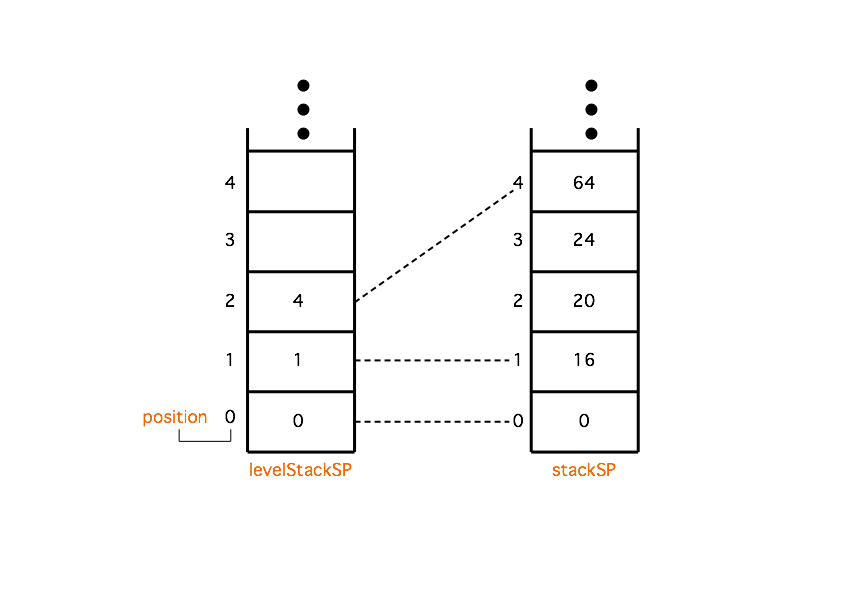
\includegraphics[width=1\textwidth]{img/stackSymbolTable.png}
    \caption{Stack structure}
    \label{fig:stack_symbol_table}
\end{figure}

In Figure ~\ref{fig:stack_symbol_table}, we see two rectangle objects. One is named ~\textit{levelStackSP} and the other is named ~\textit{stackSP}.

\begin{enumerate}
\item ArrayList$<$Integer$>$ ~\textbf{levelStackSP}
\item ArrayList$<$Integer$>$ ~\textbf{stackSP}
\end{enumerate}

The ~\textit{levelStackSP} is a stack (~\textit{ArrayList type}) which contains information about the other stack ~\textit{stackSP} (~\textit{ArrayList type}) and the main objective of this stack is to add informations related with subprogram created in the LISS code (uses a FILO system). Each ~\textbf{position} of the stack ~\textit{levelStackSP} refers to a certain level scope, so we have in this example 3 levels (level scope 0 (position 0), level scope 1 (position 1) and level scope 2 (position 2)). And each position of the stack ~\textit{levelStackSP} contains information about the position of the other stack ~\textit{stackSP}.

The stack ~\textit{stackSP} is the main stack which holds every ~\textit{push} instruction in the MIPS assembly code and behaves as a FILO system also. Each time that the compiler adds some information into the stack (regarding to the MIPS assembly code), it will also be added into the stack ~\textit{stackSP} (last free position available). Also, every ~\textit{pop} instruction, in the MIPS assembly code, will be removed as well as in the stack too (it removes the last position who has information).

To make a summary, we have two structure. One stack (~\textit{levelStackSP} ) who gives us information about the position of any subprogram that the compiler have found to the other stack ~\textit{stackSP}. And one stack (~\textit{stackSP}) who behaves the stack of MIPS architecture.

Notice that each time that the stack ~\textit{stackSP} will add some information, it will add in the next free position available and will add the amount to store with the previous position. In this example, we can see that the compiler wanted to add 40 bytes of memory. So he just added to the next free position available (position 4), 24 plus 40 bytes which is equals to 64 (see the position 4 value in the stack ~\textit{stackSP}).

Regarding to removing informations in the stack ~\textit{stackSP}, it just removes the last position who have information. When the last position of the stack ~\textit{stackSP} is linked to the stack ~\textit{levelStackSP} (in the example, position 2 of stack ~\textit{levelStackSP} is linked to position 4 of stack ~\textit{stackSP}). By removing the last information of the stack ~\textit{stackSP}, it will also remove the last information of the stack ~\textit{levelStackSP}.

\subsubsection{The algorithm for finding variables in the stack}

The algorithm of searching the position of a certain variable is simple.
Whenever we need a variable greater than the level scope 0 (variable only available in the stack MIPS architecture), we need to check at the symbol table his availability. If the variable is there, we need to check the level scope of the variable. If the level scope is greater than 0, then we need to check at our stack structure where is the position in the stack.

So, in this case, we need to check firstly the stack ~\textit{levelStackSP}. With the knowledge of the level scope of the variable, we access to the right position of that stack. Then by accessing it, we will know which position is in the other stack ~\textit{stackSP}.
By knowing the position of the stack ~\textit{stackSP}, we just need to calculate the position of the variable in the stack.
And the calculation is done by this way :

\begin{enumerate}
\item Take the last value added to the stack ~\textit{stackSP}.
\item Take the value found regarding to the variable in the stack ~\textit{stackSP}.
\item Do a substracton of those values ( step 1 - step 2 ).
\item Get the address value regarding to the variable in the symbol table.
\item Add the address value to step 3.
\item Position found in the stack.
\end{enumerate}

After that, we just need to create one mips instruction which gets the right value of the position in the stack MIPS architecture regarding to the variable.

\subsection{LISS language code generation}

This part will talk about the code generation of every statements feasible in the LISS language.
It will be divided by sections for each statements and then divided by the level scope equally to 0 or greater for a better view regarding to the complexity done with the MIPS architecture and his requirements.

\subsubsection{Creating a variable in LISS}

\begin{itemize}
\item Level scope equals to zero
\end{itemize}

Let's see an example of LISS code in Listing ~\ref{lst:declaration_variable_code_generation}.

\begin{lstlisting}[caption={Example of creating variables in LISS},label={lst:declaration_variable_code_generation}]
program liss{
  declarations
    a, b = 4, c = -1, d = +2 -> integer;
    flag, flag1 = false, flag2 = true -> boolean;
    array1, array2 = [2,1,1], array3 = [1] -> array size 3;
    array4 = [[1,2],[3]] -> array size 3,3;
    set1, set2 = { y | y+1 < y+4}, set3 = {} -> set;
    seq1, seq2 = <<1,2>> -> sequence;
  statements
}
\end{lstlisting}

In Listing ~\ref{lst:declaration_variable_code_generation}, we can see some variables being declared in the LISS code in the level scope 0.
In this case, the compiler needs to take those informations and generate them to MIPS assembly code.
Let's go line by line and explain them each one.

In line 3 of Listing ~\ref{lst:declaration_variable_code_generation}, we see 4 different named variables being declared with the type ~\textit{integer}.
The compiler adds them to the symbol table and do some checkings regarding to the semantic system implemented. Then, if everything is all right, it associate them (each variable) with a certain address to each one. Remember that the type ~\textit{integer} cost 4 bytes in the memory as explained before. So, in this case, it will generate the address 0, 4, 8 and 12 for those variables.

Also, notice that the association of those addresses are not set in the same order as the variables were declared. This is due to the fact that those variables are stored in a ~\textit{HashMap} structure where the key is the name of the variable and the value are informations regarding to the variable. And we implemented a ~\textit{HashMap} structure for the case that the line (which the compiler will process entirely) will check if names of variables are differents.

In the end, when the compiler will take the information of those variables for putting them into the symbol table and regarding to the ~\textit{HashMap} structure in JAVA which doesn't have the notion of ordering keys. It will simply take the keys in any orders and the compiler will associate those keys (the name of the variable) with an address created. 
Take care that there is no problem in doing that, because the compiler always knows the address of each variables (symbol table structure holds the information).

Later, we need to generate the assembly code if everything worked as planned. And this is done by declaring them in the data section of the MIPS assembly code (see in Listing ~\ref{lst:integer_mips_level_scope_0}).

\begin{lstlisting}[caption={Code generation of integer variables in MIPS assembly code},label={lst:integer_mips_level_scope_0}]
  .data
	a : .word 0		
	b : .word 4	
	c : .word -1		
	d : .word +2		
\end{lstlisting}

So creating variables in the level scope 0, basically means that those variables are globals.
And in this case, we add them to the ~\textit{data} section otherwise it will be in the stack.

By creating those variables, in the MIPS assembly code, the way of declaring them is different than if it was in a greater level scope.
In Listing ~\ref{lst:integer_mips_level_scope_0}, we do by associating the name of the variables (~\textit{a}) following by the size type of the variable (~\textit{.word} (4 bytes)) and  the value that the variable will store.

Notice that a variable who isn't declared will store the value 0.

In line 4 of Listing ~\ref{lst:declaration_variable_code_generation}, we create the boolean variables and this is done in the same way as an ~\textit{integer} variable.
Remember that ~\textit{boolean} types cost 4 bytes in the memory. So we just need to do the same way as if it was an ~\textit{integer} type.

We declared the name of the variable (~\textit{flag}), then we say the size type (~\textit{.word} (4 bytes)) and we write the value of the boolean (true is 1, false is 0) (see in Listing ~\ref{lst:boolean_mips_level_scope_0}).

\begin{lstlisting}[caption={Code generation of boolean variables in MIPS assembly code},label={lst:boolean_mips_level_scope_0}]
  flag : .word 0		
  flag2 : .word 1		
  flag1 : .word 0		
\end{lstlisting}

Notice that boolean variable who are not initialized, the default value is false.

In line 5 and 6 of Listing ~\ref{lst:declaration_variable_code_generation}, we declare some array type variables.
The idea of an ~\textit{array} type is a fixed-size sequential collection of elements with the same type. 
And in MIPS assembly code, there is a certain way of creating those types by doing with this way (see in Listing ~\ref{lst:array_mips_level_scope_0}).

\begin{lstlisting}[caption={Code generation of array variables in MIPS assembly code},label={lst:array_mips_level_scope_0}]
  array2 : .space 12		
  array1 : .space 12		
  array3 : .space 12		
  array4 : .space 36		
\end{lstlisting}

In Listing ~\ref{lst:array_mips_level_scope_0}, we declare the name of the variable, then the size type (sequence of memory, ~\textit{.space}) (due to the fact that it is an ~\textit{array} type) and finally, how much space that the array will store.
Take care that ~\textit{array} type in LISS, only store integer values and for calculating the space regarding to the ~\textit{array} variable, we need to do some calculation. 

The calculation is done by multiplying all the limits of the ~\textit{array} variable and with that result we multiply by the number 4 (space of an ~\textit{integer} variable).
Regarding to the line 5 in Listing ~\ref{lst:declaration_variable_code_generation}, the calculation for the variables ~\textit{array1}, ~\textit{array2} and ~\textit{array3} is done by taking the limits 3 and multiply it by 4 (space of an integer), which is equal to 12.
However regarding to line 6 in Listing ~\ref{lst:declaration_variable_code_generation}, the calculation for the variable ~\textit{array4} is done by multiplying all the limits associated to the variable (3x3 which is 9) and then, multiplying by 4 (space of an integer), which is equal to 36. And the strategy is the same if the dimension of the ~\textit{array} variable is greater regarding to the calculation of generating the space of the ~\textit{array}.

Now that we declared the space of those variables in MIPS assembly code, we need to declare the values associated to those variables.

So we implemented a system which takes the information of each position of the array regarding to the value that was declared in the array.

For example, if we have a multidimensional array with 3 dimensions like that :

\begin{lstlisting}[caption={Example of an array with 3 dimensions},label={lst:array_with_3_dimension_example}]
  array1 = [[[12]],[[5,6],[7]]] -> array size 2,2,3;
\end{lstlisting}

We need to create a system which will take the informations regarding to the array declared and this pass by taking the informations of some values who are declared in the array (see Figure ~\ref{fig:access_array_structure}).

\begin{figure}[h!]
  \centering
    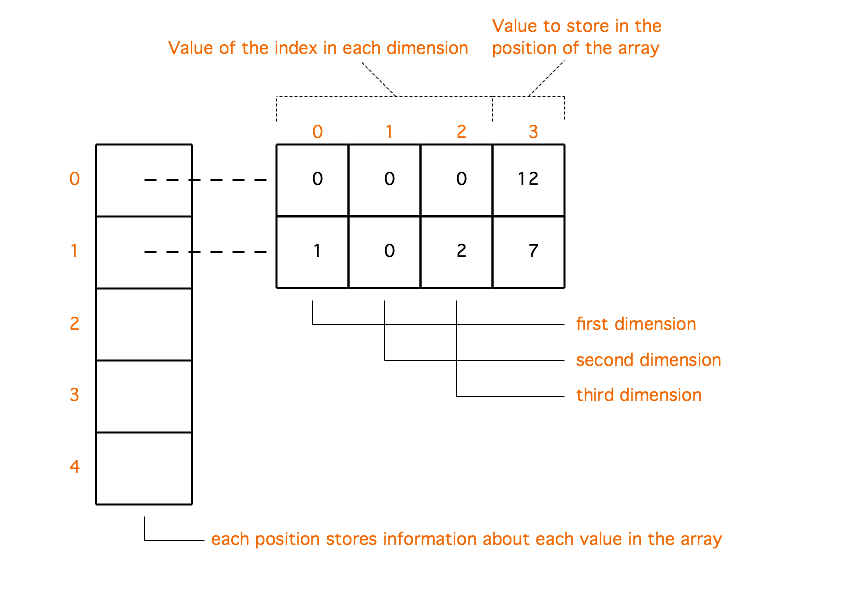
\includegraphics[width=1\textwidth]{img/access_array.png}
    \caption{Structure for saving information of each value declared in a array}
    \label{fig:access_array_structure}
\end{figure}

So we created a system which has this structure (see in Listing ~\ref{lst:access_array_structure}).

\begin{lstlisting}[caption={Structure of saving informations of each index in JAVA},label={lst:access_array_structure}]
  ArrayList<ArrayList<Integer>> accessArray
\end{lstlisting}

Basically, it is a structure where one ~\textit{ArrayList} holds the informations of one index of the array processed and add it to the other ~\textit{ArrayList} whenever it have completed to process the information (it behaves like a stack).

So, in Figure ~\ref{fig:access_array_structure}, we can see clearly that the left rectangle is the stack where each position of it, holds informations (a ~\textit{ArrayList} of integer informations) regarding to one index declared in the array.

And this ~\textit{LinkedList} of informations has a certain architecture which must be explained.
The size of that ~\textit{ArrayList} is equal to the dimension of the ~\textit{array} plus one (refers to the value available in the index processed). Then, the first positions of the ~\textit{ArrayList} are reserved for each dimension of the array and the last position of the ~\textit{ArrayList} is the value which needs to be stored in that index of the array.
Each dimension will inform us which position has the value.

For example, regarding to the example in Figure ~\ref{fig:access_array_structure}.

The first information available in the stack is in the position 0 and this information is telling us that there is a value to be stored at the position [0,0,0] with the value 12. The second information, available in the position 1 of the stack, is telling us that there is another value to be stored at the position [1,1,0] with the value 7.

After getting all those informations, we need to generate the instructions and for that we need to calculate the right position of each value with the information that it was processed.

The calculation is done with the next formula (see Equation ~\ref{eq:formulae_array_position}).

\begin{equation} \label{eq:formulae_array_position}
  p(l,a) = \sum_{i=0,\ i\neq n-1}^{n-2} (a[i]\times\prod_{j=i+1}^{n-1} l[j])+a[n-1]
\end{equation}

In Equation ~\ref{eq:formulae_array_position}, the equation needs two inputs:

\begin{itemize}
\item ~\textbf{l} - array variable which has the informations about the limits of the array in question.
\item ~\textbf{a} - array variable which has the information of the position of the array that need to be processed.
\end{itemize}

Notice that the variable ~\textbf{m}, in the equation, is equal to the dimension of the array.

Then after getting those inputs variables, it calculates the position of the array in question for any n-dimensional size.
Also, take a note that if the dimension of the array is equal to 1, the equation doesn't compute the first part (due to the restriction of the equation).

And to understand the formula, let's explain it with an example.

Imagine that we have those input variables for the formula (examples taken from Figure ~\ref{fig:access_array_structure} and Listing ~\ref{lst:array_with_3_dimension_example}):

\begin{figure}[h!]
  \centering
    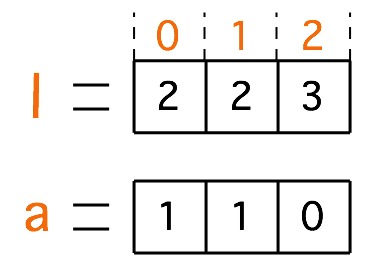
\includegraphics[width=0.2\textwidth]{img/example_position_calculation.png}
    \label{fig:example_position_calculation_structure}
\end{figure}

By using the equation above with that example, let's unroll it.

\begin{equation}
 \begin{matrix}
 \begin{aligned}
  p(l,a) &= a[0] \times l[1] \times l[2] + a[1] \times l[2] + a[2] \\
  p(l,a) &= 1 \times 2 \times 3 + 1 \times 3 + 0 \\
  p(l,a) &= 6 + 3 + 0 \\
  p(l,a) &= 9
 \end{aligned}
 \end{matrix}
\end{equation}

So, with that calculation we can see that the position of the array is the number 9.

Let's see throw the next Figure ~\ref{fig:array_example_calculation} if the calculation was done correctly.

\begin{figure}[h!]
 \centering
  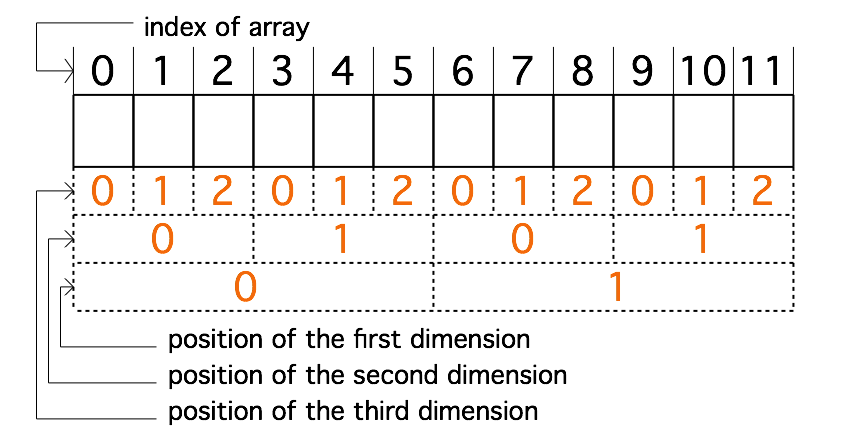
\includegraphics[width=0.8\textwidth]{img/array_example_calculation.png}
  \caption{Array structure with size 2,2,3.}
  \label{fig:array_example_calculation}
\end{figure}

Using the positions of the variable array ~\textbf{l} and using them to find the right position in the array structure in Figure ~\ref{fig:array_example_calculation}, we go firstly to the right position of the first dimension (number 1 ( l[0] = 1)). Then, we go to the second dimension of the part where belongs the number 1 in the first dimension,  in this case it is the number 1 ( l[1] = 1 ). Finally, we go to the last dimension and go to the number 0 ( l[2] = 0).  As we can see, it goes directly to the index number 9 of the array. 

This proves that the algorithm works very well and also, how it calculates the position for an array with the structure implemented in this project.

Now that we know how the position is calculated in an array; let's continue to unroll the line 5 and line 6 in Listing ~\ref{lst:declaration_variable_code_generation}.

So, after creating the space of those variables ~\textit{array2}, ~\textit{array3} and ~\textit{array4}, we need to initialize them.

Let's see an example of how it is done the initialization of arrays in Listing ~\ref{lst:array2_initialization_mips}.

\begin{lstlisting}[caption={MIPS assembly code generated for the variable array2},label={lst:array2_initialization_mips}]
  .text
    main:
       ##### Initialize Value Array :array2#####
       li $t0,2		# 5:12
       li $t1,0		# 5:12
       sw $t0, array2($t1)		
       li $t0,1		# 5:12
       li $t1,4		# 5:12
       sw $t0, array2($t1)		
       li $t0,1		# 5:12
       li $t1,8		# 5:12
       sw $t0, array2($t1)		
       #######################################
\end{lstlisting}

In MIPS architecture, it is impossible to declare the array with the values associated in the declaration parts. So, we need to fix this situation and this is done by creating MIPS assembly code in the flow of the program execution.

Basically, the idea is that the MIPS assembly code is always in the first place regarding to the flow of the program execution. In this case, we can see in Listing ~\ref{lst:array2_initialization_mips} that the MIPS assembly code for the initialization of the ~\textit{array2} variable comes first in the flow of the program execution. Then after that every initialization was made regarding to arrays, comes and begins the flow of the program execution.

In Listing ~\ref{lst:array2_initialization_mips}, let's explain how the code generation works for values regarding to the array:

\begin{itemize}
\item line 4 - Loading the value 2, this is the value to be stored in the array.
\item line 5 - Loading the position 0, this is the position which the value will be stored (use the algorithm for calculating the position).
\item line 6 - Store the value 2 to the position 0 in the array2 memory.
\item line 7.... - Continue to use the same strategy with the next values that needs to be added.
\end{itemize}

Storing one value in an array needs three MIPS instruction assembly code.

Notice that the position calculated is always multiplied, at the end, by the size of an ~\textit{integer} (number 4).

As we can see in Listing ~\ref{lst:array2_initialization_mips}, the position are :

\begin{itemize}
\item line 5 - the value is 0 =$>$ position 0 (0/4 = 0)
\item line 8 - the value is 4 =$>$ position 1 (4/4 = 1)
\item line 11 - the value is 8 =$>$ position 2 (8/4 = 2)
\end{itemize}

Also, take care that every other positions in the array have the value 0 and that is why we don't need to create the MIPS instructions for them, because the default value is 0 in an array non-initialized (the story changes when those arrays are created in a level scope greater than 0, but it will be talked further).

In line 7 of Listing ~\ref{lst:declaration_variable_code_generation}, we see two differents named variables being declared with the type ~\textit{set}.

That type basically doesn't create any informations in the MIPS assembly code for the declarations parts. Instead it saves the information in a specific structure created for that purpose. The structure is made with the concept of a Tree structure where there are some nodes with branches or not, associated to others nodes.

And this structure is made by two JAVA class:

\begin{itemize}
\item Node Class
\item Set Class
\end{itemize}

The Node JAVA class is a class where represents the concept of a node structure in a tree. It is represented by three things:
\begin{enumerate}
\item String data 
\item Node left
\item Node right
\end{enumerate}

The variable ~\textbf{data} refers to the value represented of that node, the variables ~\textbf{left} and ~\textbf{right} refers to a node who might be to the left or right side of the actual node.

Now, the Set class is a class where it saves the information of the set in a tree structure and the free variable associated with the set. Take care, that the Set class uses and abuses the Node class.
It is represented by two things:

\begin{enumerate}
\item ArrayList$<$Node$>$ identifier
\item Node head
\end{enumerate}

The variable ~\textbf{identifer} refers to a list of free variables that are stored in the tree structure. This is done for one particularly reason, instead of browsing the entire tree and looking to those free variables, we have a list where we can change the state of those free variables available in the list and directly, it changes also in the tree. The advantage of that structure is that we don't need to browse in the tree and change or look for those free variable. Otherwise it will be a time consume by doing that.

Then we have the variable ~\textbf{head} which holds the information about the head node of the tree structure.

Let's see the Set structure in Figure ~\ref{fig:set_structure}.

\begin{figure}[h!]
 \centering
  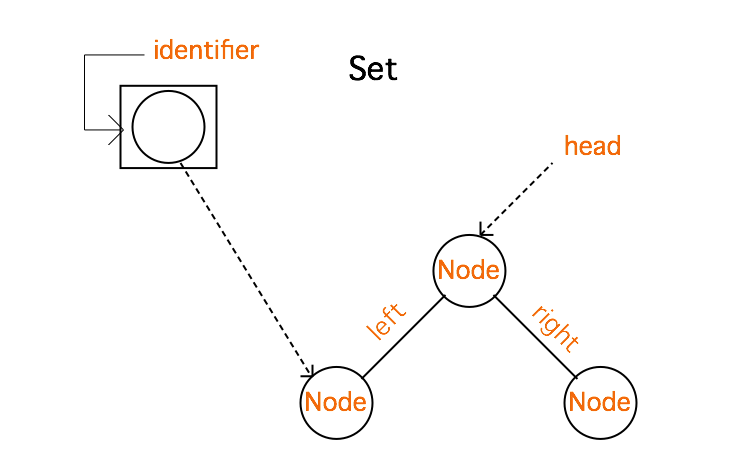
\includegraphics[width=0.8\textwidth]{img/set_structure.png}
  \caption{Set structure in JAVA}
  \label{fig:set_structure}
\end{figure}

Basically, a set in LISS is made with a tree structure where each nodes are a symbol of the expression associated with the set.
For our project, we managed to create a variable which points to the head of the tree structure (also named by the variable ~\textit{head}) and a list of free variables stored in the variable named ~\textit{identifier}.

We implemented a list for free variables for one reason and this reason comes with the fact that we can join multiple sets.
Notice that each set have their own free variable which means that each free variable regarding to each sets does have differents address. And we need to collect all those addresses of each free variable with a list.

Let's see an example of joining two sets in Figure ~\ref{fig:sets_associaton}.

\begin{figure}[h!]
 \centering
  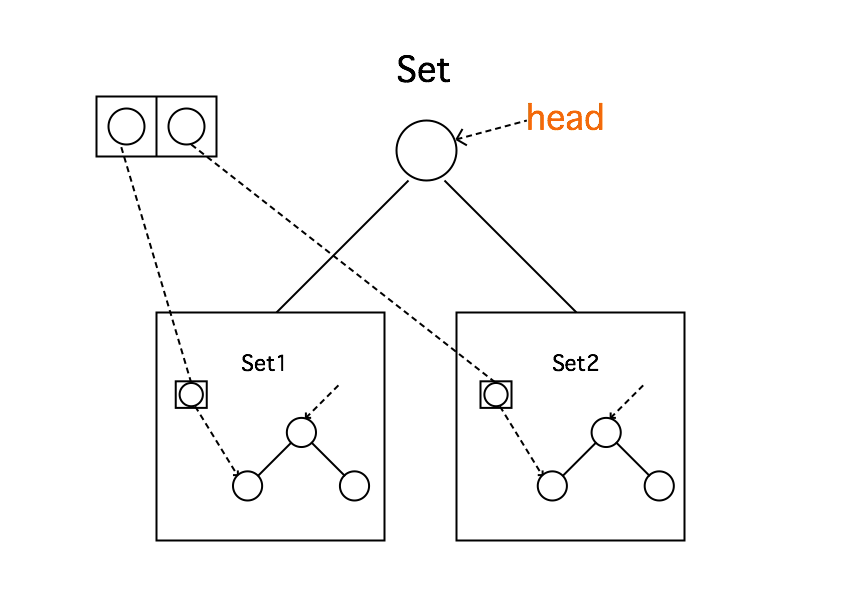
\includegraphics[width=0.8\textwidth]{img/sets_association.png}
  \caption{Set structure in JAVA}
  \label{fig:sets_associaton}
\end{figure}

In Figure ~\ref{fig:sets_associaton}, we can see that the head of the ~\textbf{Set} is connected with two sets (left and right). This means that we are joining two sets (~\textit{Set1} and ~\textit{Set2}) with the head of one ~\textit{Set}. And, in this case, we are growing the tree structure by doing more complex structure.

Doing those changes will need some attention to fix the free variables available on each sets. And this is why we have created the set class with a list of free variables. Like that, we can get the free variables from the others sets and adds them to the list of the ~\textbf{Set}. By this way, we can change the states of each free variables available in the list of ~\textbf{Set} which will also changes in the other sets too.

After that the compiler, processed the Set class for the variable, it will associate that structure to the variable added in the symbol table.

Notice that the compiler will generate some code only when it will be asked it in the ~\textit{statements} part of the LISS code.

Lastly, we need to talk about the different states that a set can have regarding to the declaration part.

Set variable can have three different states:

\begin{itemize}
\item Universe set
\item Empty set
\item Defined set
\end{itemize}

The ~\textbf{universe} set is a set which basically represent the whole number system and it is represented by this syntatic in LISS code:

\begin{lstlisting}
  set1 -> set;
\end{lstlisting}

The ~\textbf{empty} set is a set which basically represents nothing in the number systems, also considered ~\textit{null} and it is represented by this syntatic in LISS code:

\begin{lstlisting}
  set1 = {} -> set;
\end{lstlisting}

The ~\textbf{defined} set is a set which basically represents the numbers expressed with the expression associated to the set and they are defined by this way in LISS code:

\begin{lstlisting}
  set1 = {y | y+1 < y+4} -> set;
\end{lstlisting}

Let's talk finally with the last line 8 in Listing ~\ref{lst:declaration_variable_code_generation}, it represents the declaration of variables with the type ~\textit{sequence}. And the idea of generating the code for that type, is almost the same as the type ~\textit{array}.

Basically, the type ~\textit{sequence} creates one position of memory for each variable declared and will store the value -1 in there (value -1 is equal to NULL). By setting the value to -1, it means that the variable sequence is empty, no values are associated to that variable (the same as saying that the sequence wasn't intialized).

Let's see the code generated for the example available on line 8 of Listing ~\ref{lst:declaration_variable_code_generation}:

\begin{lstlisting}
  seq2 : .word -1		
  seq1 : .word -1		
\end{lstlisting}

As we can see, we create the name of the variable firstly, then the type of the variable (~\textit{.word)} and the value associated to that variable ( NULL value (-1)). Notice that the type of the variables is a 4 bytes size and this is for one main raison.

The ~\textit{sequence} type is a linkedlist of integer numbers and those numbers will be stored in the ~\textit{heap} section.
So, in this case, we need to know in which address the first element of the sequence is stored and this pass by knowing the address of the first element of the sequence. However this address must be stored at one place that can be known and this goes by storing that address to the variable name associated.

The size of an address in the MIPS architecture is 4 bytes, so in this case the variable must be 4 bytes long and that is why we choosed the type ~\textit{.word}.

After creating the variables, we need to do the same thing as the ~\textit{array} type, check if the sequence is initialized or not.

And if it is initialized, we need to generate some MIPS assembly code. 

For generating the code, we need to take the values that are associated to the sequence and generate each MIPS assembly code for each values.

Notice also, that the MIPS assembly code that will be generated, will also be placed in the same area as the initialization of an array (before the program execution code).

Let's explain it throw the example of Listing ~\ref{lst:declaration_variable_code_generation}, the code generated for the variable ~\textbf{seq2}.

\begin{lstlisting}[caption={Code generated for the sequence variable},label={lst:sequence_initialization_mips}]
 	lw $s0, seq2		
	li $s1, 1		
	jal cons_sequence		
	move $s0, $v0		
	li $s1, 2		
	jal cons_sequence		
	sw $v0, seq2		
\end{lstlisting}

Basically, in our project we need some  inputs in order to add some values to a sequence and those informations are:
\begin{enumerate}
\item the name of the variable (for having the knowledge of which sequence that the number must be associated).
\item the value that needs to be added to the sequence.
\item the function who will do the work of adding the number to the heap and linking it to the variable ~\textit{sequence}.
\end{enumerate}

So, regarding to the variable ~\textbf{seq2} in Listing ~\ref{lst:declaration_variable_code_generation}, the compiler needs to take the value 1 and 2 and generate code for them to the sequence.

In Listing ~\ref{lst:sequence_initialization_mips}, the compiler firstly creates an instruction which puts the address of the sequence variable to a saved registers (\$~\textit{s0}), then it loads the value 1 ( first number that must be added to the sequence) to the next saved registers (\$~\textit{s1}) and finally it calls the function that will add to the sequence (~\textit{cons\_sequence}).

Notice that those steps are always the same and regarding to the use of those saved registers, the reason is that we don't need to use the stack for storing the information. Instead we use some profits of the MIPS architecture, and we use those saved registers. 

Care that normally we use the saved registers for calling some functions due to the fact that those registers won't be modified within that transition of jumping to those functions. And for our case, we call the function that will add the number to the sequence.

After that the function will finish to process (~\textit{cons\_sequence} function), it will return to the register \$v0 the return value and in this case, this is the address of the first element of the sequence. Then in line 5, it will move the address of the register \$v0 to the register \$s0, due to the fact that it needs to add the second number (number 2) to the sequence. And finally, at the end it will store the address of the first element of the sequence to the sequence variable name (line 8).

\begin{itemize}
\item Level scope greater than zero
\end{itemize}

Creating variables with a level scope greater than 0 means that those variables are created in a function.
Let's see how they are created in Listing ~\ref{lst:variable_declarations_greater_than_0}.

\begin{lstlisting}[caption={Example of creating variables in a level scope greater than 0},label={lst:variable_declarations_greater_than_0}]
  program liss{
    declarations
      subprogram test(){
        declarations
          a, b = 4, c = -1, d = +2 -> integer;
          flag, flag1 = false, flag2 = true -> boolean;
          array1, array2 = [2,1,1], array3 = [1] -> array size 3;
          array4 = [[1,2],[3]] -> array size 3,3;
          set1, set2 = { y | y+1 < y+4}, set3 = {} -> set;
          seq1, seq2 = <<1,2>> -> sequence;
        statements
      }
    statements
  }
\end{lstlisting}

As we can see in Listing ~\ref{lst:variable_declarations_greater_than_0}, they are created in the same way as if it is with a level scope equals to 0. The only thing that is different is that they are created in a different area ( subprogram area ) and this means that the every declaration of variables will be declared and stored in the stack memory.

Basically, when the compiler process a function within the LISS code, it will process firstly the arguments that the function has and secondly, every variable declaration under the ~\textit{declarations} part.

When the compiler have added those informations to the symbol table, he will also calculate the total size that needs to be allocated to the stack memory in MIPS architecture.

Notice that before calculating the total size of the stack memory, the compiler has already processed the information of every variables and arguments into MIPS code instruction.

Let's see how the stack is organized in Figure ~\ref{fig:stack_architecture_mips}.

\begin{figure}[h!]
  \centering
    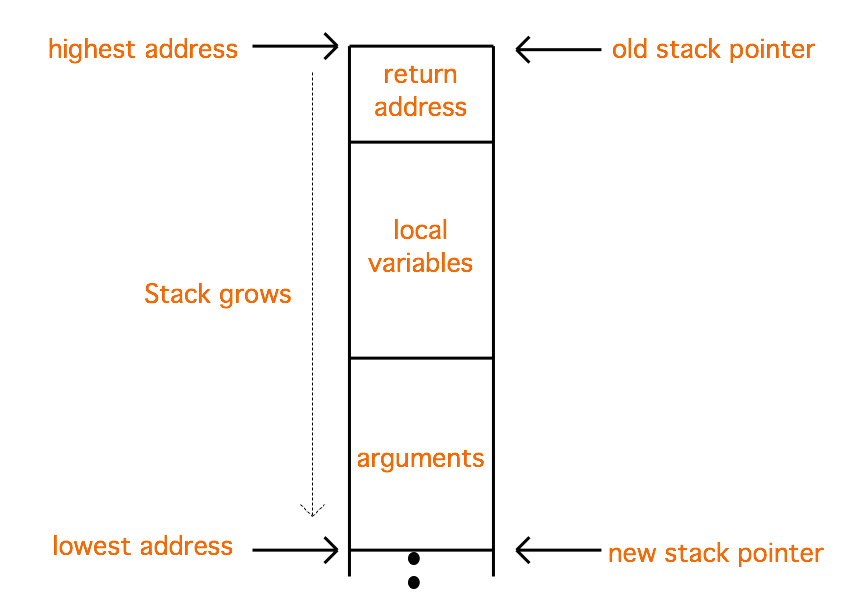
\includegraphics[width=1\textwidth]{img/stack_architecture.png}
    \caption{Architecture of the stack relatively to a function in LISS}
    \label{fig:stack_architecture_mips}
\end{figure}

So, in Figure ~\ref{fig:stack_architecture_mips}, the stack is organized by this way: 
\begin{itemize}
\item the variables of the arguments function next to the new position of the stack pointer
\item the local variables relatively to the variables declared under the declarations parts.
\item the return address of the function.
\end{itemize}

Notice that the stack grows from the highest address to the lowest one and that there is also a reason regarding to this chosen architecture.

Remember that each variables that the compiler finds and needs to add to the symbol table, an address is also associated to the variable. When the compiler enters to a function statement ( declaration of a subprogram in LISS), the address is set to zero. And in this case, each variables who are found, will begin by the address zero and then incremented relatively to their types.

Now, if we want to access to a variable in that stack, we just need to get the address of the variable throw the symbol table and get the position of the ~\textit{new stack pointer} (if the level scope of the compiler, when he is processing the access, is the same as the level scope of the variable). Then we add both of them and get the position for accessing the value of the variable in the stack.

Care that, in Figure ~\ref{fig:stack_architecture_mips}, it is possible that the arguments section or the local variables section might not appear in the stack (depending to the LISS code) and also that those informations are added to the stack created under the project.

Now, let's explain the code generated in MIPS relatively to the Listing ~\ref{lst:variable_declarations_greater_than_0}.

The fact that it is a subprogram (function), every code generated will be added relatively to the branch associated of the function name in MIPS and the first thing that must be done under that branch is to increase the stack relatively to the amount of informations that needs to be allocated (see in Listing ~\ref{lst:init_function_mips}).

\begin{lstlisting}[caption={Initialization of MIPS code generated for a function},label={lst:init_function_mips}]
    test: 
      addi $sp, $sp, -160		
      sw $ra, 156($sp)
\end{lstlisting}

In Listing ~\ref{lst:init_function_mips}, we see the name of the branch associated to the function in first. Then comes the part of adding some informations about the stack that the function needs to allocate. In this case, we have one instruction ~\textit{add} (line 2) which explains us that the function needs to allocate 160 bytes  in the stack memory regarding to the stack pointer and to refresh the address of the new stack pointer with the new allocation. Finally, we save the information regarding to the return address of the function into the stack (line 3).

Those are always the initialization of MIPS instruction regarding to a function declared in LISS. After that, comes the MIPS assembly code relatively to the variables declared under the ~\textit{declarations} part of the function.

In line 5 of Listing ~\ref{lst:variable_declarations_greater_than_0}, we are declaring integer variables and the code generated for those variables are available in Listing ~\ref{lst:integer_variable_declaration_level_scope_greater_than_0}.

\begin{lstlisting}[caption={Declaring integer variables in level scope greater than 0 on MIPS.},label={lst:integer_variable_declaration_level_scope_greater_than_0}]
  li $t0,0		
  sw $t0, 0($sp)
  li $t0,4		
  sw $t0, 4($sp)
  li $t0,-1		
  sw $t0, 8($sp)
  li $t0,+2		
  sw $t0, 12($sp)
\end{lstlisting}

In Listing ~\ref{lst:integer_variable_declaration_level_scope_greater_than_0}, line 1 and 2 are related for declaring the variable ~\textbf{a}. Basically, the idea of declaring integer variable is done by this way: 

\begin{enumerate}
\item load the value to store in the variable
\item store that value to the position related to the variable in the stack.
\end{enumerate}

Notice that the position is given by the algorithm that we explained in a previous section (stack structure).

Now, line 3 and 4 are the code generated for the variable ~\textbf{b}; line 5 and 6 are the code generated for the variable ~\textbf{c}; line 7 and 8 are the code generated for the variable ~\textbf{d}.

Line 6 of Listing ~\ref{lst:variable_declarations_greater_than_0}, refers to variables declared with the type boolean and the code generated for that type is visible in Listing ~\ref{lst:boolean_variable_declaration_level_scope_greater_than_0}.

\begin{lstlisting}[caption={Declaring boolean variables in level scope greater than 0},label={lst:boolean_variable_declaration_level_scope_greater_than_0}]
  li $t0,0		
  sw $t0, 16($sp)
  li $t0,1		
  sw $t0, 20($sp)
  li $t0,0		
  sw $t0, 24($sp)
\end{lstlisting}

In Listing ~\ref{lst:boolean_variable_declaration_level_scope_greater_than_0}, the methodology of creating boolean variables is the same as if it was with a level scope equals to zero. The only thing that differs, is the instruction for storing the value that is associated to the variable.

Line 1 and 2 of Listing ~\ref{lst:boolean_variable_declaration_level_scope_greater_than_0} refers to the declaration of the variable ~\textbf{flag}; line 3 and 4 is the declaration of the variable ~\textbf{flag2} and line 5 and 6 is the declaration of the variable ~\textbf{flag1}.

Line 7 and 8 of Listing ~\ref{lst:variable_declarations_greater_than_0}, refers to variables declared with the type array and the code generated for the variable ~\textbf{array2} is visible in Listing ~\ref{lst:array_variable_declaration_level_scope_greater_than_0}.

\begin{lstlisting}[caption={Declaring array variables in level scope greater than 0},label={lst:array_variable_declaration_level_scope_greater_than_0}]
  ##### Initialize Array :array2#####
  li $t0,0		
  sw $t0, 28($sp)
  li $t0,0		
  sw $t0, 32($sp)
  li $t0,0		
  sw $t0, 36($sp)
  #######################################
  ##### Initialize Value Array :array2#####
  li $t0,2		
  li $t1,0		
  li $t2,28		
  add $t1, $t1, $t2	
  add $t1, $t1, $sp
  sw $t0, ($t1)
  li $t0,1		
  li $t1,4		
  li $t2,28		
  add $t1, $t1, $t2	
  add $t1, $t1, $sp
  sw $t0, ($t1)
  li $t0,1		
  li $t1,8		
  li $t2,28		
  add $t1, $t1, $t2	
  add $t1, $t1, $sp
  sw $t0, ($t1)
  #######################################
\end{lstlisting}

So the creation of a variable with the type array is done almost by the same way as if it was with a variable declared in the level scope equals to zero.
But it differs on some points which must be explained.

As we know, the stack grows and decrease by time and the values in the memory of the stack are not removed regarding to the process of the stack by growing up or decreasing it. So, regarding to variables with the type of array, we need to firstly set to zero all the position of the array in the stack (done on line 2 to 7 of Listing ~\ref{lst:array_variable_declaration_level_scope_greater_than_0}). Then, we need to put the values that were declared in the array to their right position.

Let's see how it is done with the value 2 of the variable ~\textbf{array2} relatively with the code made in Listing ~\ref{lst:array_variable_declaration_level_scope_greater_than_0}:

\begin{enumerate}
\item line 10 : Put the value 2 to register.
\item line 11 : Put the index of the value 2 regarding to the array declared to register.
\item line 12 : Put the address of the array to register.
\item line 13 : Sum the index with the address of the array for getting the address of the index.
\item line 14 : Sum the index address with the stack pointer, for getting the address position in the stack.
\item line 15 : Store the value 2 to the address position in the stack.
\end{enumerate}

And redo the same algorithm for the next values that need to be stored. Also notice that the index of the array is calculated throw the algorithm mentioned before and that the address of the array is associated to the variable and caught with the symbol table.

Line 9 of Listing ~\ref{lst:variable_declarations_greater_than_0}, refers to the declaration of variables with the type set and it only gets and creates the tree structure which will be associated to each variables. Nothing more will be generated as code, unless if it is used in the ~\textit{statements} section.

Line 10 of Listing ~\ref{lst:variable_declarations_greater_than_0}, refers to the declaration of variables with the type sequence and the code generated for the variable ~\textbf{seq2} is visible in Listing ~\ref{lst:sequence_variable_declaration_level_scope_greater_than_0}.

\begin{lstlisting}[caption={Declaring sequence variable in level scope greater than 0},label={lst:sequence_variable_declaration_level_scope_greater_than_0}]
  li $t2,-1		
  sw $t2, 148($sp)		
  lw $s0, 148($sp)	
  li $s1, 1		
  jal cons_sequence		
  move $s0, $v0		
  li $s1, 2		
  jal cons_sequence		
  sw $v0, 148($sp)		
\end{lstlisting}

The idea of  generating the code for the sequence variable is the same as an array variable.
Firstly, we need to put the value NULL in the stack memory (line 2 and 3 of Listing ~\ref{lst:sequence_variable_declaration_level_scope_greater_than_0}) and then, if some values are associated to the variable, we need to generate the code (which is almost the same way as if it was on a level scope equals to 0).

So, firstly we go get the address of the variable sequence which needs to add a certain value (line 4 of Listing ~\ref{lst:sequence_variable_declaration_level_scope_greater_than_0}), then we load the value to a register (line 5 of Listing ~\ref{lst:sequence_variable_declaration_level_scope_greater_than_0}) and finally, we call the function that will process the concatenation of the value to the sequence.

Notice that after creating those generated code relatively to those variable declarations, comes the flow of the execution subprogram (everything that is created under the statements part of the subprogram). Finally, at the end of the execution of the subprogram, we need to remove the allocated stack memory of the function and return.

Let's see the code generated in Listing ~\ref{lst:exit_function_mips}.

\begin{lstlisting}[caption={Exiting the function in MIPS assembly code},label={lst:exit_function_mips}]
  lw $ra, 156($sp)		
  addi $sp, $sp, 160		
  jr $ra	
\end{lstlisting}

In Listing ~\ref{lst:exit_function_mips}, line 1 will get the return address of the function; then at line 2 it will remove the stack allocated for the function and finally at line 3, it will process for exiting the function with the return address.

\subsubsection{Creating I/O in LISS}

%\begin{itemize}
%\item Level scope equals to zero
%\end{itemize}

Let's see an example of LISS code in Listing ~\ref{lst:io_statements_mips}.

\begin{lstlisting}[caption={Example of I/O statements in LISS},label={lst:io_statements_mips}]
  write();
  write(a);
  write("hello");
  writeln();
  writeln(a);
  writeln("hello");
  input(a);
\end{lstlisting}

Firstly, let's talk about the output statements. They are known by ~\textit{write} and ~\textit{writeln}.

~\textit{Write} statement is an output which only prints the content and doesn't add the return carriage. However ~\textit{writeln} statement is an output which prints the content and add the return carriage at the end.

Those output statements have three possibility of being declared:

\begin{enumerate}
\item empty (line 1 and 4 of Listing ~\ref{lst:io_statements_mips})
\item expression (line 2 and 5 of Listing ~\ref{lst:io_statements_mips})
\item string (line 3 and 6 of Listing ~\ref{lst:io_statements_mips})
\end{enumerate}

Basically, for generating each output statements, we need to generate firstly the code regarding to the content available in the parentheses and then the code related to the type of output statements is available.

If the output of the statement is a ~\textit{write}, then the code will be :

\begin{lstlisting}
  jal write
\end{lstlisting}

Otherwise if the output of the statement is a ~\textit{writeln}, then the code will be :

\begin{lstlisting}	
  jal writeln
\end{lstlisting}

Notice that the behavior of the output statement ~\textit{writeln} reuses the ~\textit{write} statement plus adds the instruction code for adding the carriage return (see Listing ~\ref{lst:example_writeln_mips}).

\begin{lstlisting}[caption={Code generated for line 6 in Listing ~\ref{lst:io_statements_mips}},label={lst:example_writeln_mips}]
  la $a0, writestring0
  li $v0, 4
  jal write	
  jal writeln
\end{lstlisting}

And the code already predifined regarding to both of the statement is available in Listing ~\ref{lst:write_writeln_mips}.

\begin{lstlisting}[caption={MIPS assembly code of write and writeln},label={lst:write_writeln_mips}]
  write: 
	syscall
	jr $ra
  writeln: 
	li $v0, 4
	la $a0, newline
	syscall
	jr $ra
\end{lstlisting}

Now, let's talk about the input statement which is known by ~\textit{input}.

The idea behind of that statment for generating the code, it is to call the function which process for the output in MIPS and then store the information to the variable that is associated to the ~\textit{input} statment inside of the parentheses.

Let's see the code generated of line 7 in Listing ~\ref{lst:io_statements_mips} below:

\begin{lstlisting}
  jal read		
  move $t0, $v0		
  sw $t0, a		
\end{lstlisting}

As we can see, after processing the read statement. We need to move the value that the user have put to another register and finally, store the value to the variable that was associated.

This is the code that is predefined for the read statement (see in Listing ~\ref{lst:read_mips}).

\begin{lstlisting}[caption={Read statement code in MIPS},label={lst:read_mips}]
  read: 
    li $v0,4
    la $a0,messagereadvalue
    syscall
    li $v0,5
    syscall
    jr $ra
\end{lstlisting}

\subsubsection{Creating conditional statement in LISS}

Creating a conditional statement in LISS is basically following that schema available in Figure ~\ref{fig:conditional_figure}.

\begin{figure}[h!]
  \centering
    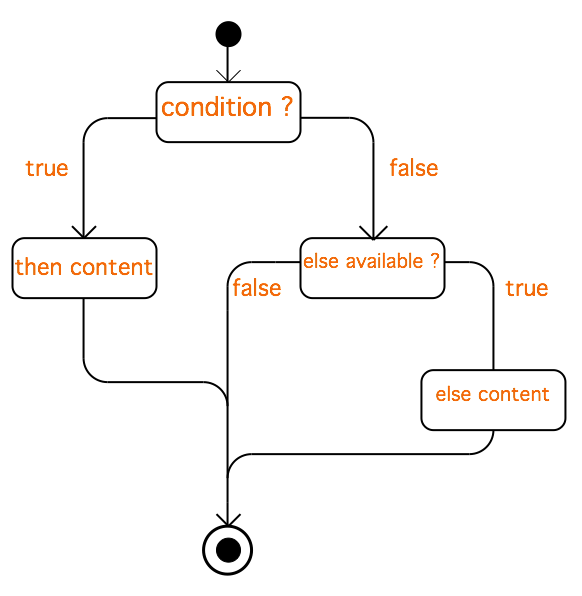
\includegraphics[width=0.7\textwidth]{img/conditional_statement.png}
    \caption{Schema of the conditional statements in LISS}
    \label{fig:conditional_figure}
\end{figure}

And for a better view of how it is generated let's see an example of a conditional statement in Listing ~\ref{lst:conditional_statement_liss}.

\begin{lstlisting}[caption={Example of conditional statement in LISS},label={lst:conditional_statement_liss}]
  if(flag)
  then{
    writeln("Then content.");
  }else{
    writeln("Else content.");
  }
\end{lstlisting}

Basically we have, in Listing ~\ref{lst:conditional_statement_liss}, a conditional statement with an if and an else statement. The condition of the if-statement  in this case is false, so by this way the else content will be processed when it will be executed.

Now let's see how the code is generated in Listing ~\ref{lst:conditional_code_generation}.

\begin{lstlisting}[caption={Code generated for conditional statement in MIPS},label={lst:conditional_code_generation}]
    lw $t0,flag		
    bne $t0, 1, else1		
    la $a0, writestring0
    li $v0, 4
    jal write		
    jal writeln		
    j l1		
  else1:		
    la $a0, writestring1
    li $v0, 4
    jal write		
    jal writeln		
  l1:		
\end{lstlisting}

In Listing ~\ref{lst:conditional_code_generation}, line 1 is the piece of code relatively to the condition of the conditional statement, then comes at line 2 the instruction which compares the value of the condition to the value true. If the value are different then it must jump to the else-condition. Otherwise if the value are the same, then it process the next instruction available in line 3 which is the code instruction available in the content of the then-statment. At the end of the then-statement, it exit the conditional statement (line 7).

Now, if the condition of the statement is true, then it will jump to the branch of the else-statement (line 8) and execute every code instruction available there. Notice that it won't jump at the end as if it will be with the then-statement content, it will process the next instruction sequentially without jumping.

Let's consider now that in the LISS code, no else-statement is used. Then the only thing that disappears is the whole code below of the else branch in Listing ~\ref{lst:conditional_code_generation}.

Let's see an example of the same code relatively to Listing ~\ref{lst:conditional_code_generation} without the else-statement in Listing ~\ref{lst:conditional_statement_no_else_mips}.

\begin{lstlisting}[caption={Code generated for conditional statements without an else-statement in MIPS},label={lst:conditional_statement_no_else_mips}]
    lw $t0,flag		
    bne $t0, 1, else1		
    la $a0, writestring0
    li $v0, 4
    jal write		
    jal writeln		
    j l1		
  else1:
\end{lstlisting}

\subsubsection{Creating iterative statement}

In LISS, we have three different ways of creating iterative statement. 

They are known by:

\begin{enumerate}
\item For-loop with 'in' condition.
\item For-loop with 'inArray' condition.
\item While-loop.
\end{enumerate}

In Figure ~\ref{fig:for-loop_in}, we can see the routine of a for-loop with an 'in' condition.

\begin{figure}[h!]
  \centering
    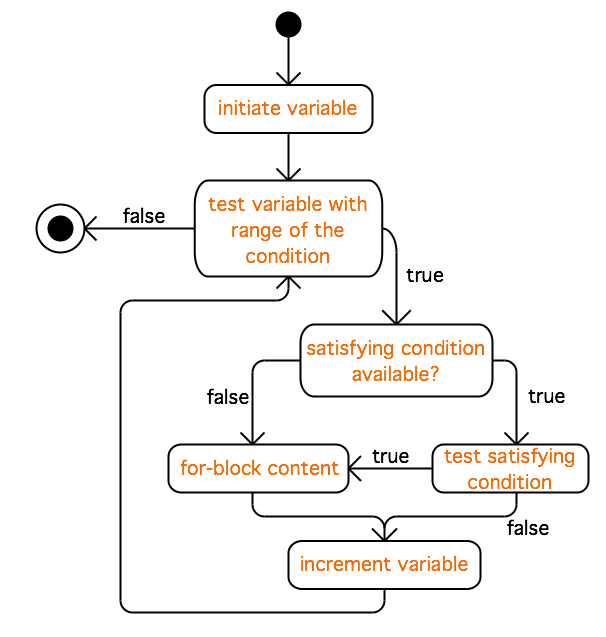
\includegraphics[width=0.8\textwidth]{img/for-loop_in.png}
    \caption{Schema of the for-loop statement relatively with the use of the condition 'in'}
    \label{fig:for-loop_in}
\end{figure}

Notice that the black circle is where the flow of the for-loop statement begins and that the double circle is where it finish of executing the flow of the for-loop statement.

Let's see a piece of LISS code relatively to a for-loop statement with an 'in' condition in Listing ~\ref{lst:for-loop_in_condition_LISS}.

\begin{lstlisting}[caption={Example of a for-loop statement with 'in' condition in LISS},label={lst:for-loop_in_condition_LISS}]
  for(a in 1..5) stepUp 1 satisfying flag==true{
    writeln(a);
  }
\end{lstlisting}

We can see in Listing ~\ref{lst:for-loop_in_condition_LISS}, that it is created a for-loop statement with an 'in' condition and beside that there is also more informations relatively to that loop. Informations that refers about the method for incrementing (~\textit{stepUp}) and a condition which must be tested every time before executing the block content inside of the for-loop statement (~\textit{satisfying}).

Let's see the code generated for that piece of code in Listing ~\ref{lst:for-loop_in_condition_mips}.

\begin{lstlisting}[caption={Code generated for the LISS code in Listing ~\ref{lst:for-loop_in_condition_LISS}},label={lst:for-loop_in_condition_mips}]
    li $t0,1		
    sw $t0, a		
  for_loop1:
    lw $t0,a		
    li $t1,5		
    slt $t0, $t1, $t0	
    sltu $t0, $zero, $t0	
    xori $t0, $t0, 1	
    bne $t0, 1, for_exit1		
    lw $t0,flag		
    li $t1,1		
    slt $t2, $t0, $t1	
    sltu $t2, $zero, $t2	
    xori $t2, $t2, 1	
    slt $t3, $t1, $t0	
    sltu $t3, $zero, $t3	
    xori $t3, $t3, 1	
    and $t2, $t2, $t3	
    move $t0, $t2		
    bne $t0, 1, satisfying_exit1		
    lw $t0,a		
    move $a0, $t0		
    li $v0, 1
    jal write		
    jal writeln		
 satisfying_exit1:
    lw $t1,a		
    li $t2,1		
    add $t1, $t1, $t2	
    sw $t1, a		
    j for_loop1		
  for_exit1:
\end{lstlisting}

In Listing ~\ref{lst:for-loop_in_condition_mips}, line 1 to 2 we create the variable ~\textit{a}; line 3 we create the for-loop branch; line 4 to 9 we test if the value of the variable ~\textit{a} is in the range of the for-loop condition. If no, we exit the for-loop flow by going to the branch named ~\textit{for\_exit1}(line 32); otherwise we continue the flow of the for-loop execution by going to line 10. Line 10 to 20 refers to the ~\textit{satisfying} condition. If the condition isn't satisfied then it goes to the branch named ~\textit{satisfying\_exit1}, otherwise it continues the flow of the execution in line 21. Line 21 to 25 is the code contained in the block of the for-loop statement. Notice that line 27 to 30 is the piece of code who will increment the variable ~\textit{a} relatively to ~\textit{stepUp}. At the end (line 31), it jumps to the branch of the for-loop statement ~\textit{for\_loop1}(line 3).

Notice also, that ~\textit{stepUp} and ~\textit{satisfying} informations are optional statement. If the satisfying statement is not available then the line from 10 to 20 and line 26 of Listing ~\ref{lst:for-loop_in_condition_mips} will be removed. Regarding to the ~\textit{step} statement, even if the information is not available, by definition a for-loop statement needs to  have some kind of iteraction by step by step. So, by omission, it will increment the variable by one; otherwise if the information is available, it will increment or decrease relatively the information shown.

In Figure ~\ref{fig:for-loop_inArray}, we can see the routine of a for-loop with an 'inArray' condition.

\begin{figure}[h!]
  \centering
    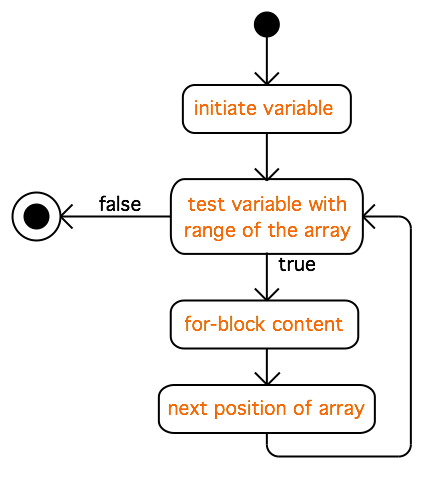
\includegraphics[width=0.5\textwidth]{img/for-loop_inArray.png}
    \caption{Schema of the for-loop statement relatively with the use of the condition 'inArray'}
    \label{fig:for-loop_inArray}
\end{figure}

The idea of that for-loop statement is to have some kind of a foreach statement in LISS. Basically, the for-loop statement will pass to every positions of the array. Notice that when it is used that for-loop statement, it is unavailable for the user of declaring any ~\textit{step} or ~\textit{satisfying} statement.

Let's see a piece of LISS code relatively to a for-loop statement with an 'inArray' condition in Listing ~\ref{lst:for-loop_inArray_condition_LISS}.

\begin{lstlisting}[caption={Example of a for-loop statement with 'inArray' condition in LISS},label={lst:for-loop_inArray_condition_LISS}]
  for(a inArray array1){
      writeln(a);
  }
\end{lstlisting}

We can see in Listing ~\ref{lst:for-loop_inArray_condition_LISS}, that it is created a for-loop statement where the ~\textit{array1} is the variable of type array and the variable ~\textit{a} will have the value of each position of the variable ~\textit{array1}.

By doing a ~\textit{writeln(a)} in line 2 of Listing ~\ref{lst:for-loop_inArray_condition_LISS}, it will output the value of each position of the array named ~\textit{array1}.

Let's see the code generated for that piece of code in Listing ~\ref{lst:for-loop_inArray_condition_MIPS}.

\begin{lstlisting}[caption={Code generated for the LISS code in Listing ~\ref{lst:for-loop_inArray_condition_LISS}},label={lst:for-loop_inArray_condition_MIPS}]
    li $t0,0		
    sw $t0, for_var4		
  for_loop4:
    lw $t0,for_var4		
    li $t1,16		
    slt $t0, $t1, $t0	
    sltu $t0, $zero, $t0	
    xori $t0, $t0, 1	
    bne $t0, 1, for_exit4		
    lw $t0,for_var4		
    lw $t0, array1($t0)		
    sw $t0, a		
    lw $t0,a		
    move $a0, $t0		
    li $v0, 1
    jal write		
    jal writeln		
    lw $t1,for_var4		
    li $t2,4		
    add $t1, $t1, $t2	
    sw $t1, for_var4		
    j for_loop4		
  for_exit4:
\end{lstlisting}

In Listing ~\ref{lst:for-loop_inArray_condition_MIPS}, line 1 to 2 we create a variable named ~\textit{for\_var4} which will be used for accesing each index of the array; line 3 we create the branch name relatively to the for-loop statement; line 4 to line 9 we test if the variable ~\textit{for\_var4} is in the limits of the array. If it isn't then it must exit the for-loop statement by going to the branch named ~\textit{for\_exit4} (line 23), otherwise it continues the flow of the execution of the code to line 10. Line 10 to line 12, we refresh the value of the variable ~\textit{a} by getting the value throw the index (variable ~\textit{for\_var4}) of the array. Line 13 to 17, this is where the content of the block relatively to the for-loop statement that will be put. In this case, it is the code instruction for writing to the output the variable ~\textit{a}. Line 18 to 21, we refresh the variable ~\textit{for\_var4} to the next position of the array and this is done by summing up with 4 bytes relatively to the old value of the variable ~\textit{for\_var4}. Lastly, line 22, we jumps to the branch ~\textit{for\_loop4} and continue the flow of the execution of the for-loop statement.

In Figure ~\ref{fig:for-loop_inArray}, we can see the routine of a while-loop.

\begin{figure}[h!]
  \centering
    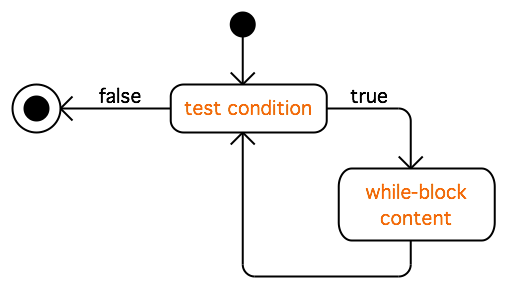
\includegraphics[width=0.6\textwidth]{img/while-loop.png}
    \caption{Schema of the while-loop statement}
    \label{fig:for-loop_inArray}
\end{figure}

Basically, behind the idea of being the most simple iterative statement, the behavior of the while-loop statement is to check the truth of the condition every iteraction. If it is true, then the content who is inside will be executed otherwise it will exit the while-loop statement.

Let's see a piece of LISS code relatively to a while-loop statement in Listing ~\ref{lst:while-loop_LISS}.

\begin{lstlisting}[caption={Example of a while-loop statement in LISS},label={lst:while-loop_LISS}]
  while(flag){
      writeln("Hello");
  }
\end{lstlisting}

In Listing ~\ref{lst:while-loop_LISS}, we have a variable ~\textit{flag} which hold the value true. In this case, the condition is true and then it should proceed to the content available inside of the parentheses. Otherwise if the condition is false, then it will quit the while-loop statement.

Let's see the code generated for that piece of code in Listing ~\ref{lst:while-loop_LISS}.

\begin{lstlisting}[caption={Code generated for the LISS code in Listing ~\ref{lst:while-loop_LISS}},label={lst:while-loop_MIPS}]
  while5:		
    lw $t0,flag		
    bne $t0, 1, while_exit5	
    la $a0, writestring0
    li $v0, 4
    jal write		
    jal writeln		
    j while5		
  while_exit5:		
\end{lstlisting}

In Listing ~\ref{lst:while-loop_MIPS}, line 1 is created for the branch name of the while-loop statement. Firstly, we incorporate the code of the condition associated to the while-loop statement (line 2), then we test the truth of the condition in line 3. If the condition is false, it will jump to the branch ~\textit{while\_exit5} (line 9) for exiting the while-loop statement; otherwise, it will continue the flow of the execution by going to line 4. At this part, it is included all the code relatively to the content available in the while-loop statement (line 4 to 7). Finally, at line 8, it will jump back to the branch ~\textit{while5} and redo the algorithm.

\subsubsection{Creating increment or decrement variables}

If we wanna increment an integer variable, we can use and do by this following way in Listing ~\ref{lst:succ_LISS}.

\begin{lstlisting}[caption={Increment variable in LISS},label={lst:succ_LISS}]
  succ i;
\end{lstlisting}

Basically, we use the word ~\textit{succ} to give notion of incrementing and then we write the variable which will be incremented (~\textit{i}).

Let's see the piece of LISS code relatively to Listing ~\ref{lst:succ_LISS} in Listing ~\ref{lst:succ_MIPS}.

\begin{lstlisting}[caption={Code generated for the LISS code in Listing ~\ref{lst:succ_LISS}},label={lst:succ_MIPS}]
  lw $t0,i		
  li $t1,1		
  add $t0, $t0, $t1	
  sw $t0, i		
\end{lstlisting}

In Listing ~\ref{lst:succ_MIPS}, line 1 load the variable ~\textit{i} to register; line 2 load the value 1 to register; line 3 add both last registers (value of the variable and the value 1); line 4 refresh and store the result to the variable ~\textit{i}.

If we wanna decrement an integer variable, we can use and do by this following way in Listing ~\ref{lst:pred_LISS}.

\begin{lstlisting}[caption={Decrement variable in LISS},label={lst:pred_LISS}]
  pred i;
\end{lstlisting}

We use the word ~\textit{pred} for decrementing the variable and then we write the variable which will be drecremented (~\textit{i}).

Let's see the piece of LISS code relatively to Listing ~\ref{lst:pred_LISS} in Listing ~\ref{lst:pred_MIPS}.

\begin{lstlisting}[caption={Code generated for the LISS code in Listing ~\ref{lst:pred_MIPS}},label={lst:pred_MIPS}] 
  lw $t0,i		
  li $t1,1		
  sub $t0, $t0, $t1	
  sw $t0, i		
\end{lstlisting}

In Listing ~\ref{lst:pred_MIPS}, line 1 load the variable ~\textit{i} to register; line 2 load the value 1 to register; line 3 subtract both last registers (value of the variable and the value 1); line 4 refresh and store the result to the variable ~\textit{i}.

\subsubsection{Assigning some values}


























%The lexical syntax is usually a regular language, with the grammar rules consisting of regular expressions; they define the set of possible character sequences that are used to form individual tokens or lexemes. A lexer recognizes strings, and for each kind of string found the lexical program takes an action, most simply producing a token.


%\chapter{Applications}
%        Application of main result (examples and case studies)
%\section{Introduction}
%\section{Summary}


%%%%%%%%%%%%%%%%%%%%%%%%%%%%%%%%%%%%%%%%%%%%%%%%%%%%%%%%%%

\chapter{SDE: DEVELOPMENT}

Before we try to explain the concept of a Syntax-Directed Editor (SDE) ~\citep{RT89b,Ko05,alsCH10a,TR81a,RMT86a,RT89a,AHW89}, let's start defining what is an Integrated Development Environment (IDE).

An IDE is described as a software application that provides facilities to computer programmers for software development. It consists , normally, of a source code editor, a compiler, a debugger, and others tools.
IDEs are designed for maximizing the productivity of programmers with visual interface and contains, normally, an interpreter, a compiler or both (see Figure~\ref{fig:ideXCode}).
%IDEs are designed for maximizing the productivity of programmers with visual interface and contains, normally, an interpreter, a compiler or both (see Figure~\ref{fig:ideXCode}).


\begin{figure}[h!]
  \centering
    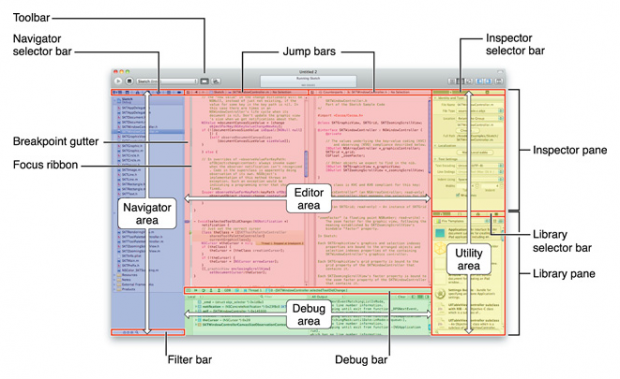
\includegraphics[width=1\textwidth]{img/XCode-interface.png}
    \caption{Example of an IDE visual interface (XCode) \protect\footnote{http://www.alauda.ro/wp-content/uploads/2011/04/XCode-interface-e1302035068112.png}}
    \label{fig:ideXCode}
\end{figure}

\newpage

Programs are created top down in the editor sections by inserting statements and expressions at the right cursor position of the current syntactic template and we can, by the cursor, change simply from one line of text to another one.

A SDE has the same approach of an IDE which is (as said above) an interactive programming environment with integrated facilities to create, edit, execute and debugging programs.
The difference between them is that SDE encourages the program writing at a high level of abstraction, and promotes the programming based on a step by step refinement process.

It liberates the user from knowing the language syntactic details while editing programs.

SDE is basically guided by the syntactic structure of a programming language in both editing and execution. It is a hybrid system between a tree editor and a text editor.

The notion of cursor is really important in the context of SDE because, when the editing mode is on, the cursor is always located in a placeholder of a correct template (see next section) and the programmer may only change to another correct template at that placeholder or to its constituents.%, and not simply from one line of text to another as an IDE alike .
%And the only place where the cursor can move anywhere is in a phrase, which can only be placed at the leftmost symbol of a template or a placeholder.

It reinforces the idea that the program is a hierarchical composition of syntactic objects, rather than a sequence of characters.

\section {What is a template?}

The grammar of a programming language is a collection of production (or derivation rules) that state how a non-terminal symbol (LHS) is decomposed in a sequence of other symbols (RHS). A template is just the RHS of a grammar rule.
Templates cannot be altered, they have placeholders for inserting a phrase or another template and they are generated by editor commands, according to the grammar production. %verificar se pode ou nao inserir placeholders


%meter example of templates !
\begin{lstlisting}[caption={Example of a IF Conditional template},label={lst:template}]
IF( condition )
  THEN statement
  ELSE statement
\end{lstlisting}

In Listing ~\ref{lst:template} we can see the editor template for the if-statement, where \textit{condition} and \textit{statement} are placeholders.

The notion of template is very important because templates are always syntactically correct for two reasons:

\begin{enumerate}
  \item First, the command is validated to guarantee that it inserts a template permitted. %at the current cursor.

  \item Second, the template is not typed, so it contains no lexical errors.

\end{enumerate}

So a correct program (i.e., a valid sentence of the programming language) is created by choosing templates and replacing placeholders by others templates or by concrets values (numeric or string constants or identifiers).

%For a better vision of the context of a SDE, see the figure ~\ref{fig:SDE}.

To clarify the definition of SDE, we will explain it with the help of an example.

\begin{figure}[h!]
  \centering
    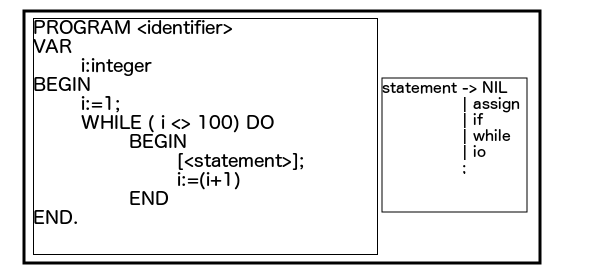
\includegraphics[width=1\textwidth]{img/SDE.png}
    \caption{SDE example}
    \label{fig:SDE}
\end{figure}

%\newpage

Figure ~\ref{fig:SDE} shows the main window of a standard Syntax-Directed Editor.
In this figure, two boxes are displayed.
The left one is the editor window where we code the program, and the right one exhibits templates choices.

Every \texttt{<}...\texttt{>}  tag represents a placeholder, and [...] represents the actual cursor position.

As the cursor changes its position, moving from one placeholder to another placeholder, the right box will be updated according to the grammar rules in the context of the new cursor position.
In this example, the cursor in Figure ~\ref{fig:SDE} is placed at the placeholder corresponding to a \textit{statement}; at the same time, the right box will be updated with all the possibile templates according to the \textit{statement} derivation rules (RHS).

To sum up, this is how a SDE works.

\section{Conception of the SDE}

By taking the ideas talked in the previous section, we managed to create a simple and ease use of a syntax directed editor based with the idea of supporting those notions:

\begin{itemize}
\item having a visualization of generating the rules with the language associated to the program (LISS).
\item seeing the code produced relatively to the rules generated.
\item having syntax, semantic errors output and results of the execution code.
\end{itemize}

And by this way, it was done by creating the program called ~\textit{liss$|$SDE} (see Figure ~\ref{fig:LISS-SDE}).

\begin{figure}[h!]
  \centering
    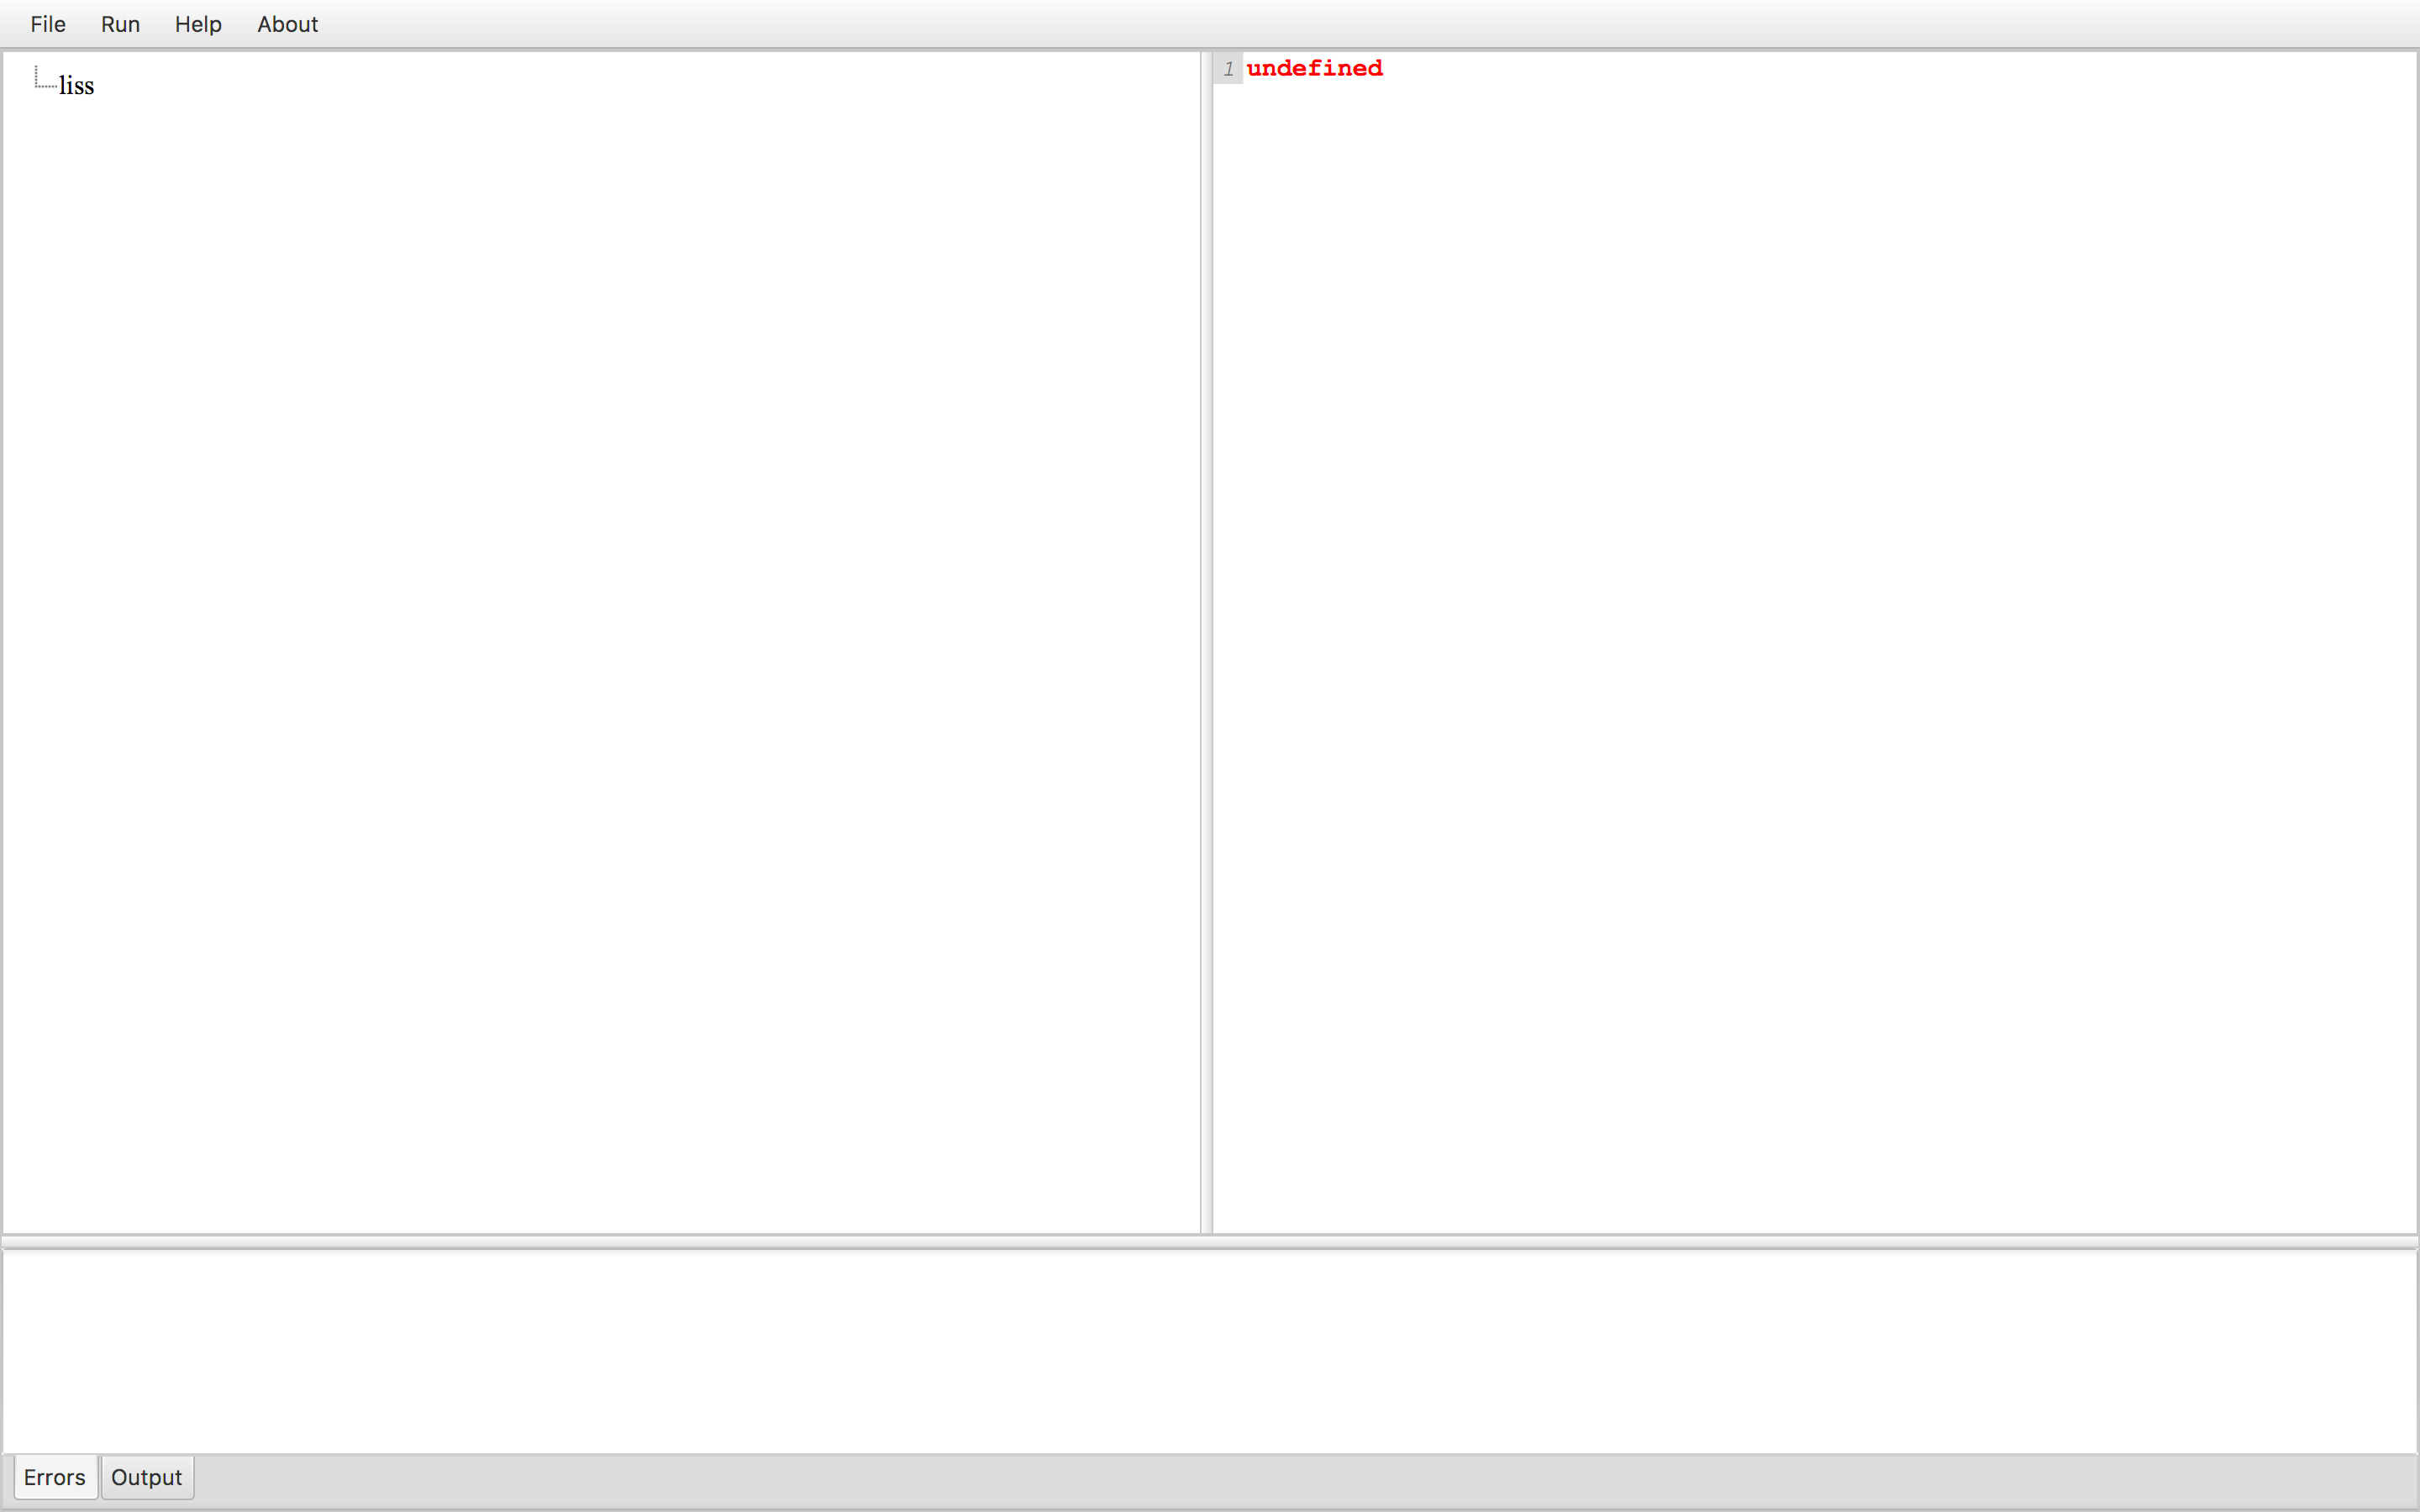
\includegraphics[width=1\textwidth]{img/LISS-SDE.png}
    \caption{liss$|$SDE}
    \label{fig:LISS-SDE}
\end{figure}

The program ~\textit{liss$|$SDE} is divided by three main areas (see Figure ~\ref{fig:LISS-SDE_structure}).

\begin{figure}[h!]
  \centering
    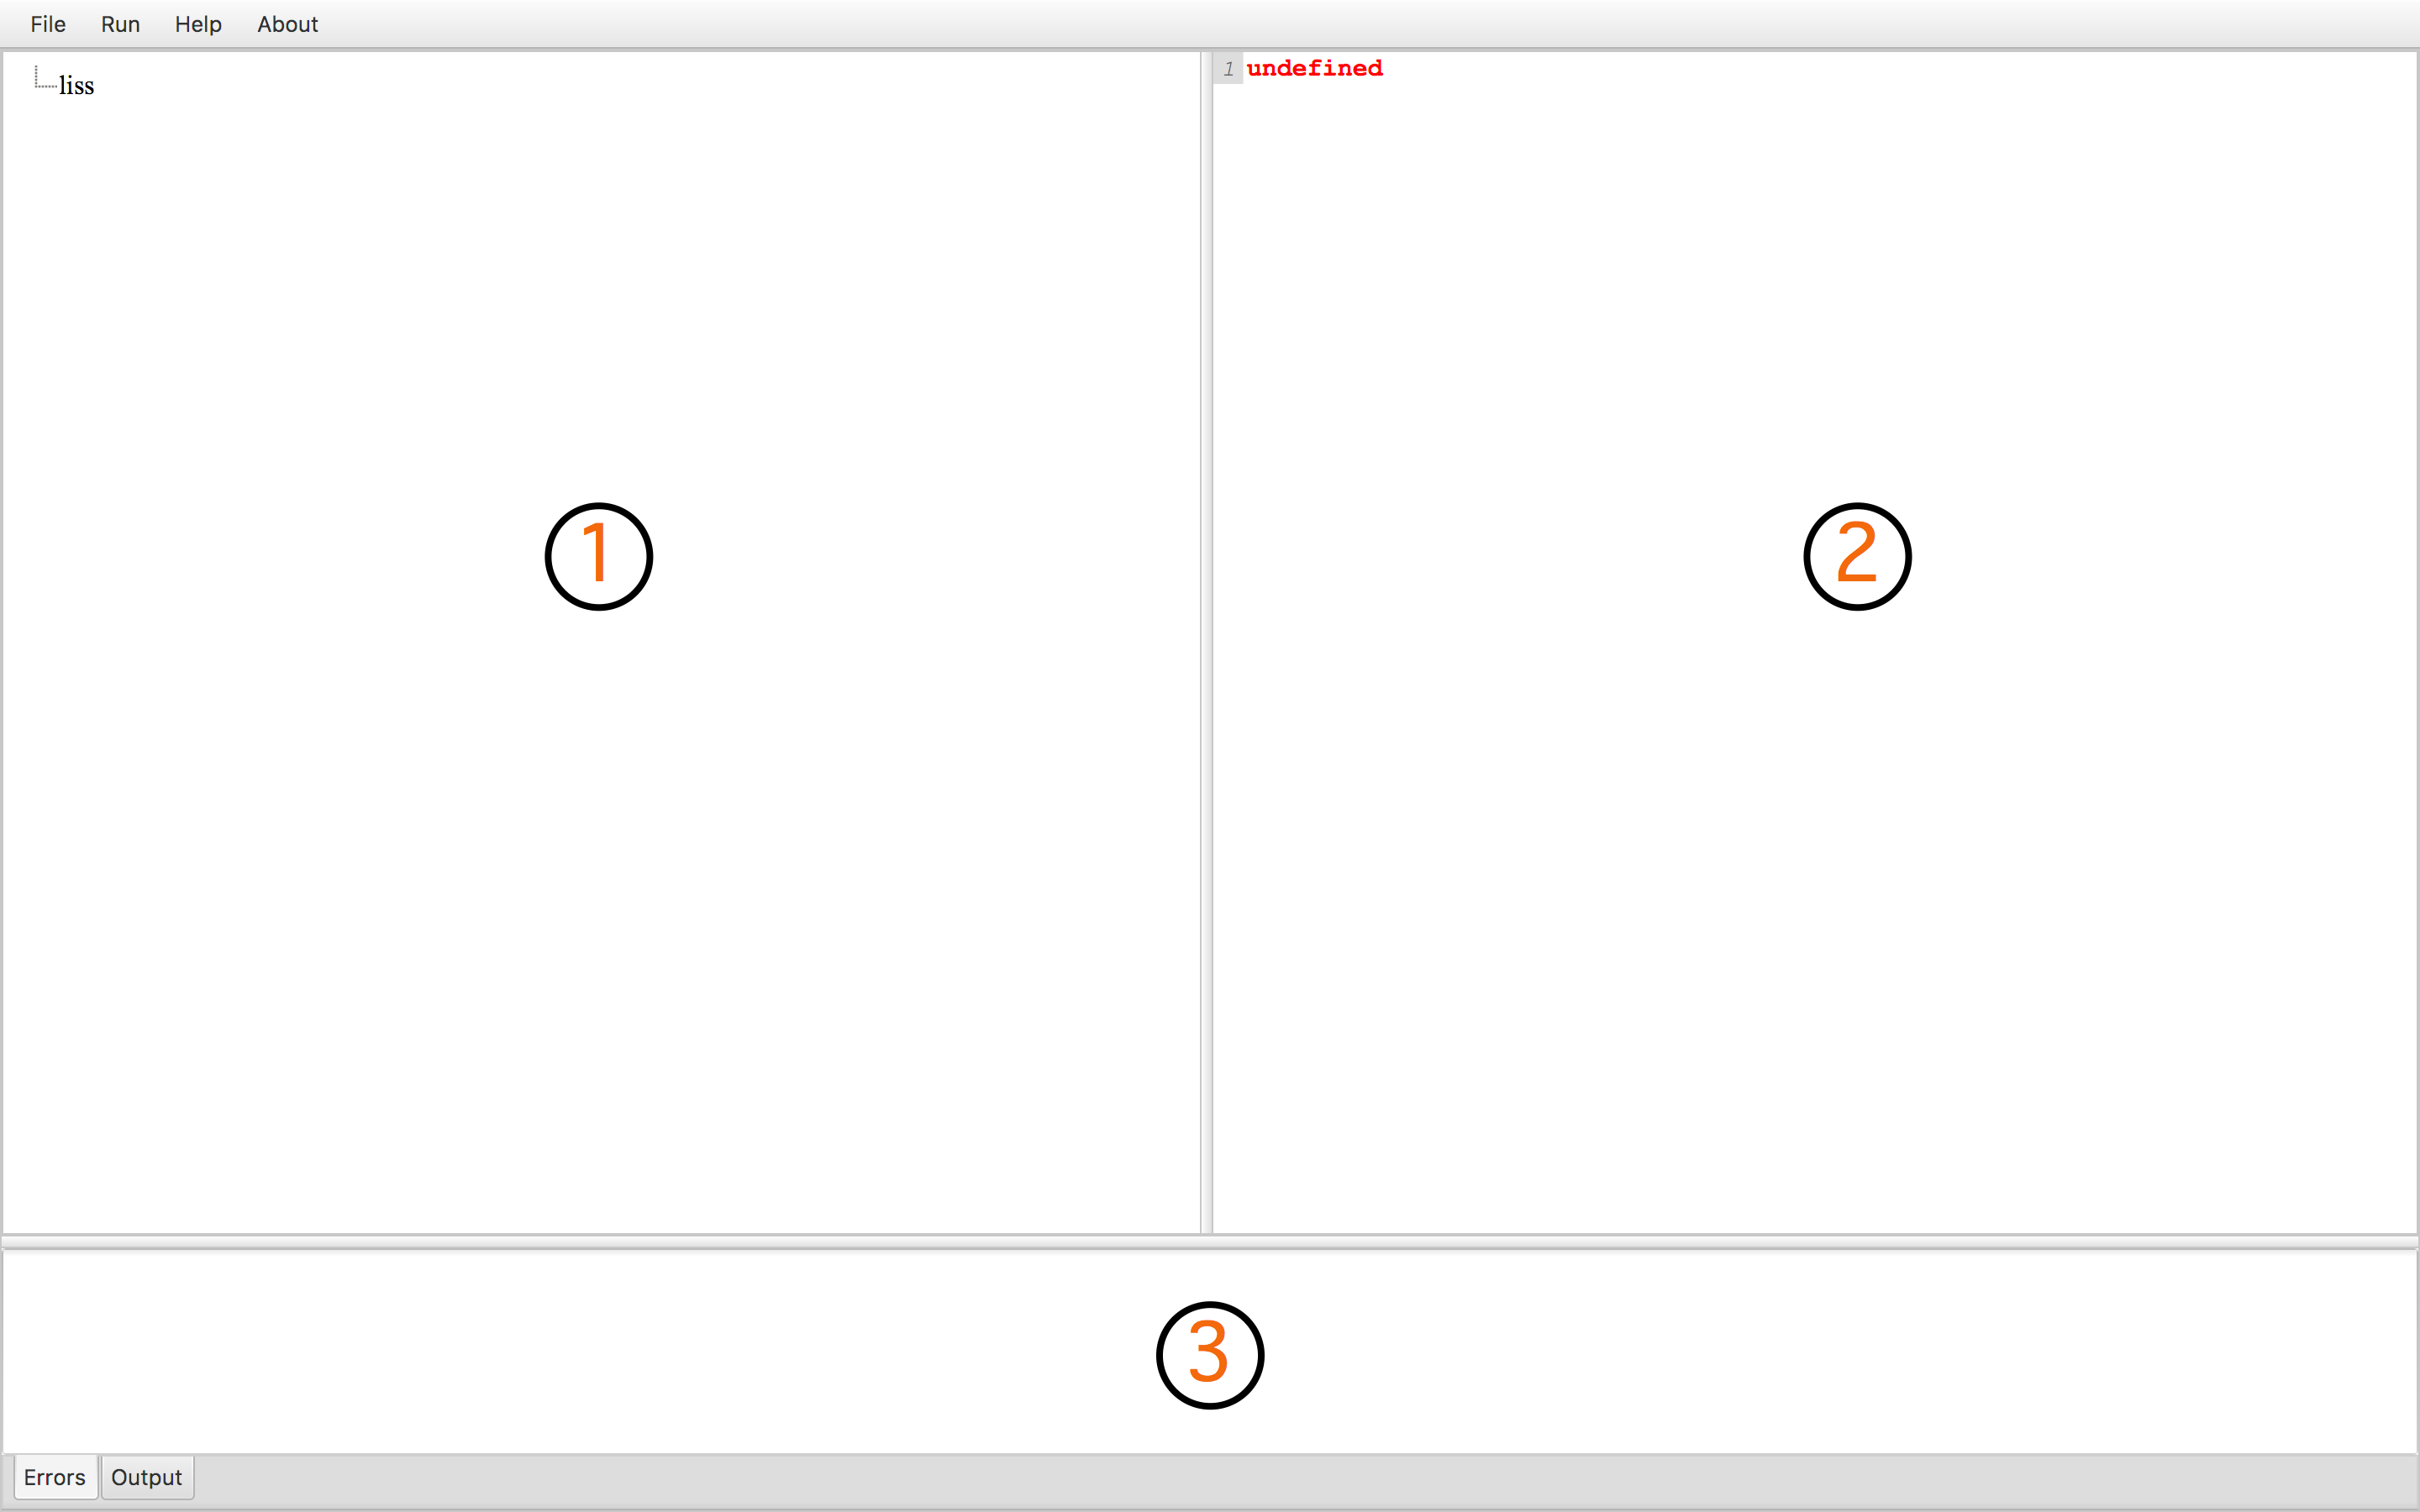
\includegraphics[width=1\textwidth]{img/LISS-SDE_organization.png}
    \caption{liss$|$SDE structure}
    \label{fig:LISS-SDE_structure}
\end{figure}

The number 1, in Figure ~\ref{fig:LISS-SDE_structure}, is where the rules of the language LISS are available. This part was implemented with the technology called HTML and Javascript, and the main reason of implementing that part with that technology was the fact that we needed to implement a tree visualization structure. 

Creating some visualization content within the JAVA context is really hard and not easy, for that reason we decided to use another technology where JAVA could handle it. And for that job, HTML and Javascript was the perfect key for creating those contents, due to his powerful and ease use of creating some visualization content.

Also, notice that, we implemented a tree visualization structure for one simple reason: a programming language is represented by a tree structure. So we decided to adapt it and create a tree visualization structure.

The number 2, in Figure ~\ref{fig:LISS-SDE_structure}, is where the code of the language is processed regarding to the rules generated to the view number 1. Notice that each time, the user generates a rule, in the same time it will refresh the view number 2.

Lastly, the number 3 is related to every syntax and semantic errors, as well as, the output of the execution relatively to the LISS code.

\subsection{Creating a program}

For a better view of that section, let's see a simple piece of LISS code in Listing ~\ref{lst:liss_sde_simple}.

\begin{lstlisting}[caption={LISS code},label={lst:liss_sde_simple}]
  program helloWorld{
    declarations
    statements
      writeln("Hello World!");
  }
\end{lstlisting}

In Listing ~\ref{lst:liss_sde_simple}, we created a 'hello world' program in LISS which basically outputs the string "Hello World!".

Now, let's try and create the same LISS code relatively with the program ~\textit{liss$|$SDE}.

%So, firstly, we need to generate the rule regarding to the LISS language and, by this way we need to interact with the view number 1 from Figure ~\ref{fig:LISS-SDE_structure}.

In Figure ~\ref{fig:LISS-SDE_example_1}, we left click in the non-terminal ~\textit{liss} which generate the rule and adds three branches under the non-terminal ~\textit{liss}:

\begin{itemize}
\item program
\item name
\item body
\end{itemize}

The ~\textit{program} word is a terminal which can be seen by his bold and blurry visual; instead that the others branches are non-terminal (~\textit{name} and ~\textit{body}) and they are not bolded nor blurried. Those visual effects are really important for the user because it means that terminal aren't clickable and non-terminal are clickable.

Notice, also, that by generating the ~\textit{liss} rule, in the right window, the code is also being refreshed and that the name of the terminal word appears correctly and non-terminal word doesn't appear with the correct name. And this is due for one reason (relatively to the behavior of the non-terminal), it means that the non-terminal must be generated and that the code isn't valid in this state.


\begin{figure}[h!]
  \centering
    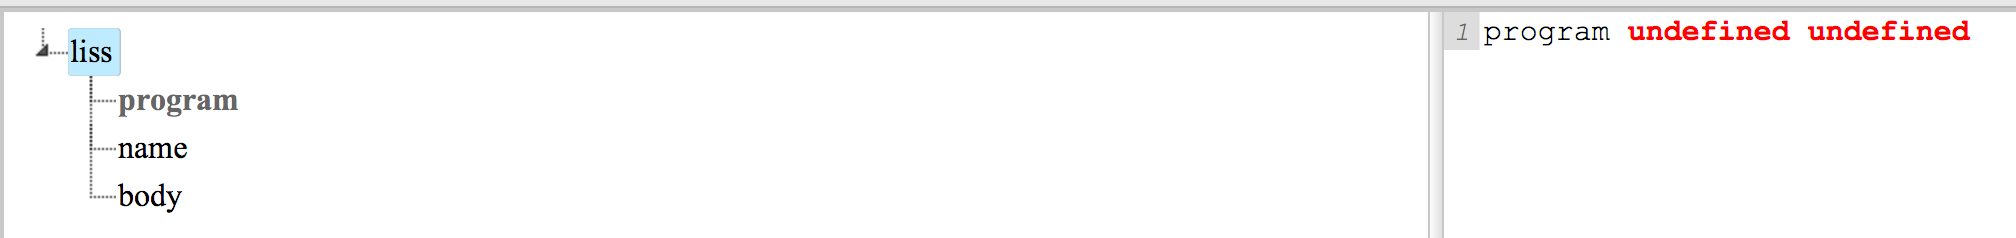
\includegraphics[width=1\textwidth]{img/LISS-SDE_creating_program/LISS-SDE1.png}
    \caption{Example of creating a LISS code (1/17)}
    \label{fig:LISS-SDE_example_1}
\end{figure}

So, in this case, we need to generate those non-terminal rules and we will do it by clicking with the left click of the mouse to the ~\textit{name} branch.
This generates a rectangle box with a name included inside of the box (called as ~\textit{IDENTIFIER} box), see Figure ~\ref{fig:LISS-SDE_example_2}.

Basically, a rectangle as shown in Figure ~\ref{fig:LISS-SDE_example_2} means that this is an input interaction with the user and that the word ~\textit{IDENTIFIER} informs to the user which kind of information must be typed.

In this case, the ~\textit{IDENTIFIER} word explains to the user that it must be typed a word which governs a certain pattern:

\begin{lstlisting}
  ('a'..'z'|'A'..'Z')('a'..'z'|'A'..'Z'|'0'..'9'|'_')*
\end{lstlisting}

\begin{figure}[h!]
  \centering
    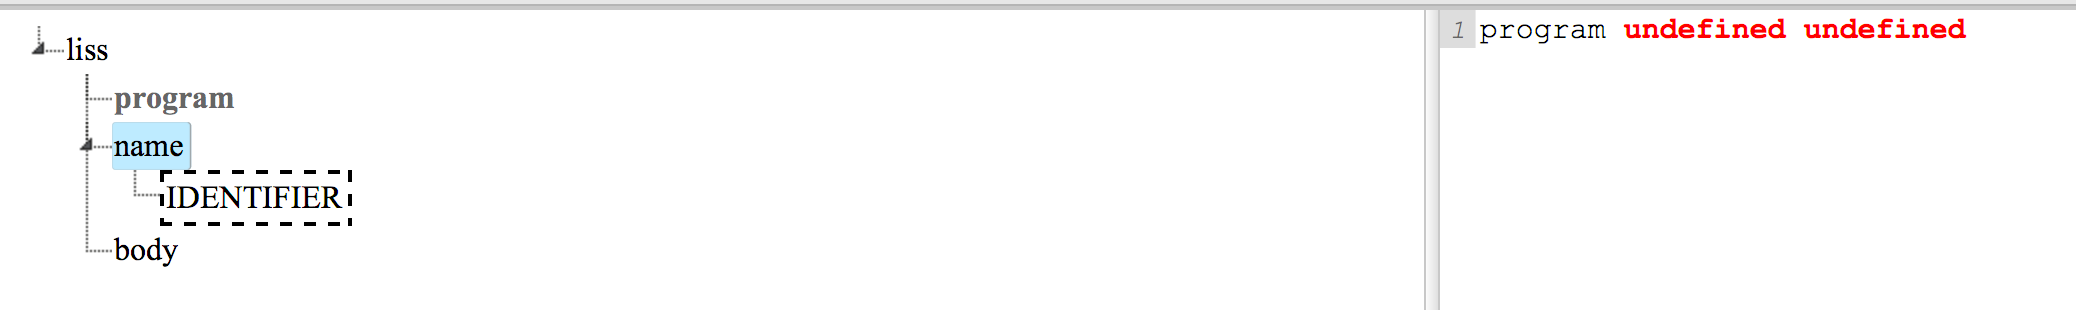
\includegraphics[width=1\textwidth]{img/LISS-SDE_creating_program/LISS-SDE2.png}
    \caption{Example of creating a LISS code (2/17)}
    \label{fig:LISS-SDE_example_2}
\end{figure}

If the pattern isn't correct relatively to the user input, then the box will change the color and put it as red (see Figure ~\ref{fig:LISS-SDE_example_3}).

Red color means that there is a problem according to the input; instead that green color means that the input is correct.

\begin{figure}[h!]
  \centering
    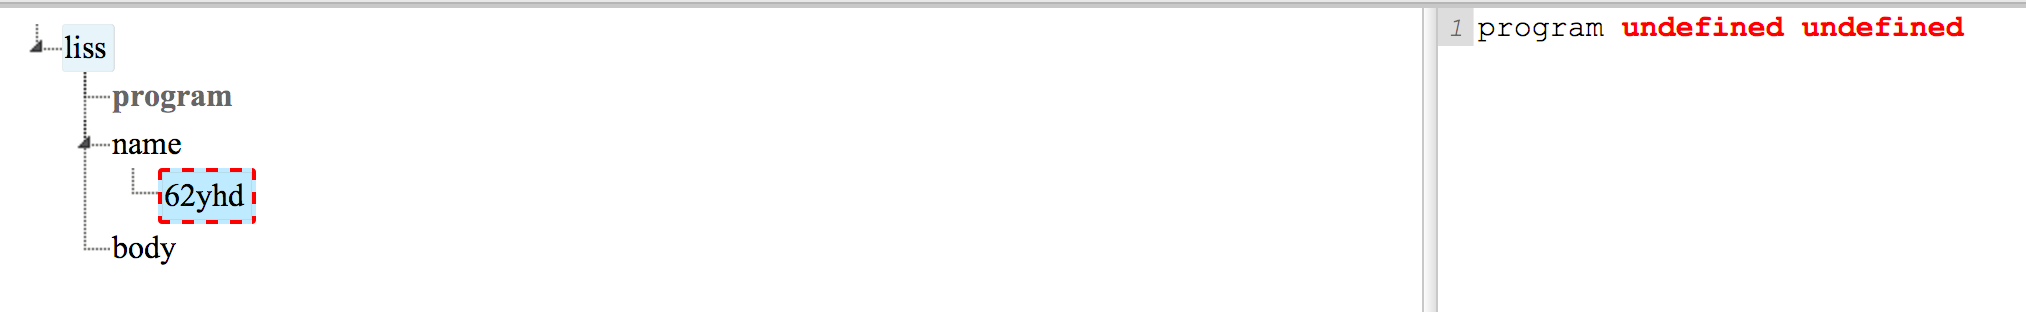
\includegraphics[width=1\textwidth]{img/LISS-SDE_creating_program/LISS-SDE3.png}
    \caption{Example of creating a LISS code (3/17)}
    \label{fig:LISS-SDE_example_3}
\end{figure}

Although, if the color of the box is green (see Figure ~\ref{fig:LISS-SDE_example_4}) then the input is correct and the ~\textit{undefined} word who was available in the right window previously (see Figure ~\ref{fig:LISS-SDE_example_3}), will change to the according name of the input.

\begin{figure}[h!]
  \centering
    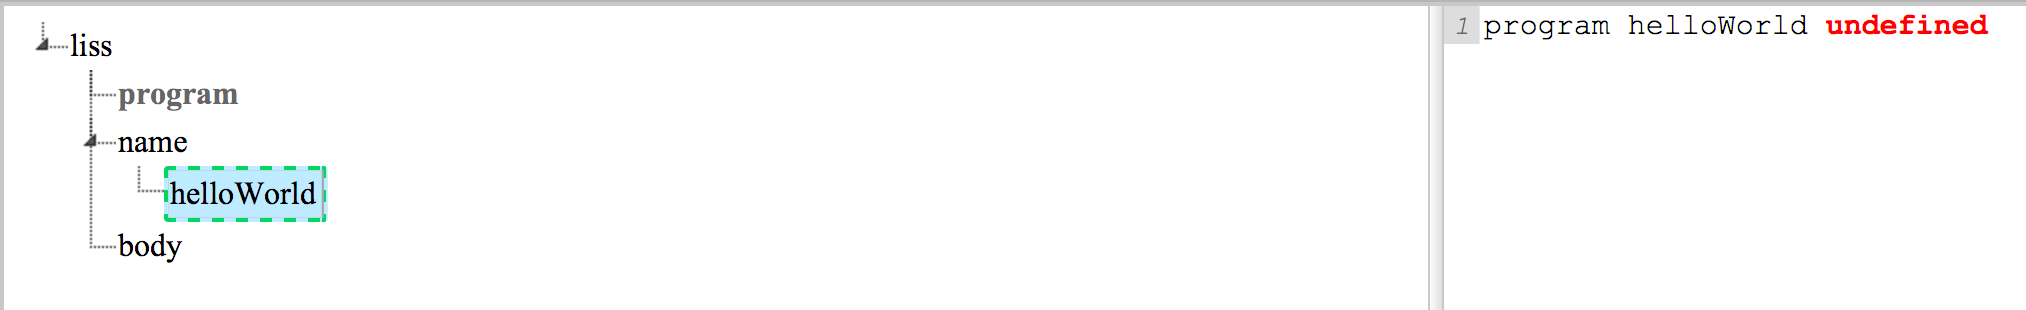
\includegraphics[width=1\textwidth]{img/LISS-SDE_creating_program/LISS-SDE4.png}
    \caption{Example of creating a LISS code (4/17)}
    \label{fig:LISS-SDE_example_4}
\end{figure}

Now, let's proceed with the other branch ~\textit{body} by clicking it with the left click. 

As we can see, in Figure ~\ref{fig:LISS-SDE_example_5}, the rule generated more rules and notice, that in the right windows, it has changed the code and that we must to generate more rules in order to make the code feasable.

\begin{figure}[h!]
  \centering
    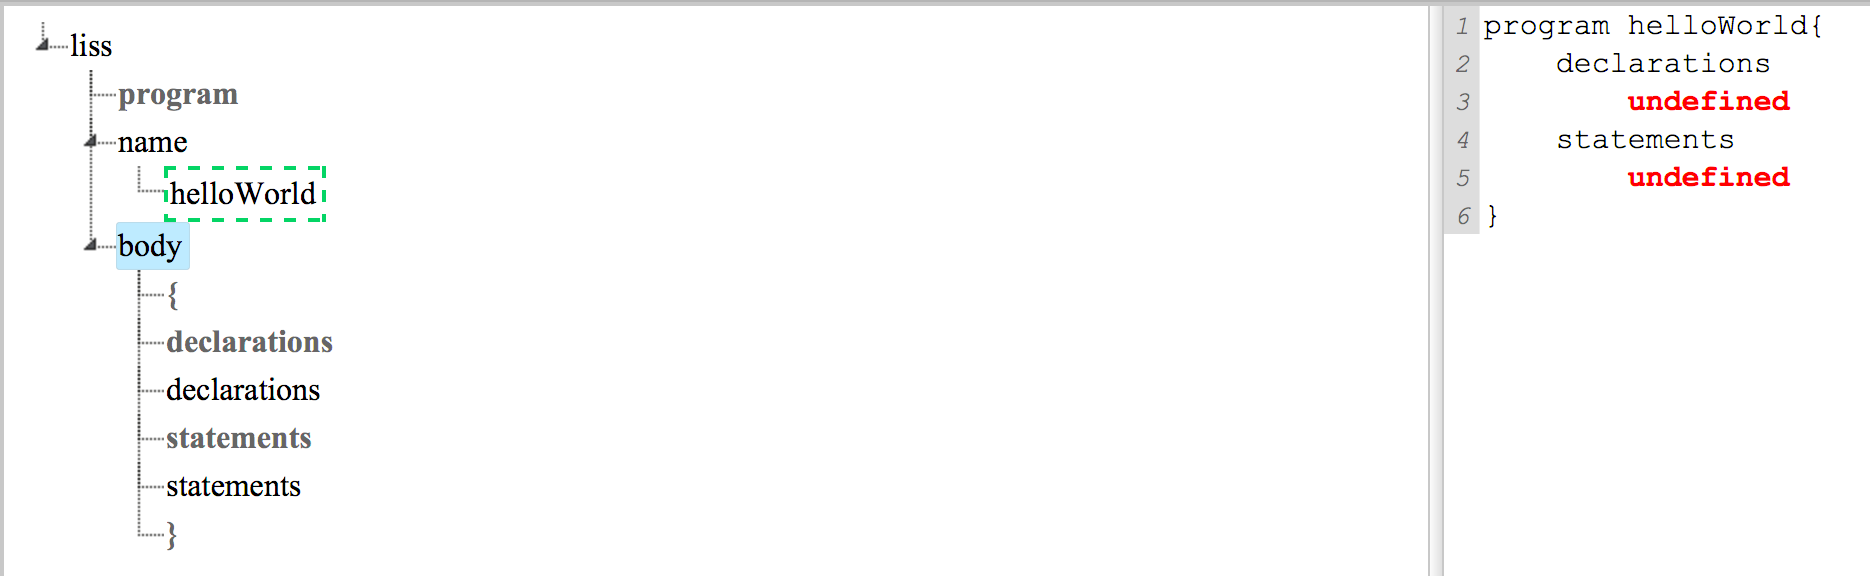
\includegraphics[width=1\textwidth]{img/LISS-SDE_creating_program/LISS-SDE5.png}
    \caption{Example of creating a LISS code (5/17)}
    \label{fig:LISS-SDE_example_5}
\end{figure}



\subsection{Executing the program}









%%%%%%%%%%%%%%%%%%%%%%%%%%%%%%%%%%%%%%%%%%%%%%%%%%%%%%%%%%

\chapter{Conclusion}
        %Conclusions and future work.
\section{Future Work}
%\section{Conclusion}
%\section{Prospect for future work}

	\bookmarksetup{startatroot} % Ends last part.
	\addtocontents{toc}{\bigskip} % Making the table of contents look good.
	%\cleardoublepage

	%- Bibliography (needs bibtex) -%
	\bibliography{dissertation}

	% Index of terms (needs  makeindex) -------------
	%\printindex
	
	
	% APPENDIX --------------------------------------
	\umappendix{Appendix}
	
	% Add appendix chapters
	\chapter{Liss Context Free Grammar}

	LISS ~\citep{CH07a} is an imperative programming language, defined by the Language Processing members (Pedro Henriques and Leonor Barroca) at UM for teaching purposes.
	It allows handling integers, sets of integers, dynamic sequences, complex numbers, polynomials, etc., etc~\citep{CH07d,CH07a,CH06a,CH06b,CH05a}.

	The idea behind the design of LISS language was to create a simplified version of the more usual imperative languages although combining functionalities from various languages.

	%explicar que é uma GIC de liss escrita em notaçao antlr.	
	
	\lstinputlisting[label={lst:GIC_LISS}]{lissGIC.g4}

	%\chapter{Support material}
	Auxiliary results which are not main-stream; or

	%\chapter{Details of results}
	Details of results whose length would compromise readability of main text; or

	%\chapter{Listings}
	Specifications and Code Listings: should this be the case; or

	%\chapter{Tooling}
	Tooling: Should this be the case.

	%Anyone using \Latex\ should consider having a look at \TUG,
	%the \tug{\TeX\ Users Group}


	% Back Cover -------------------------------------------
	\umbackcover{
	NB: place here information about funding, FCT project, etc in which the work is framed. Leave empty otherwise.
	}


\end{document}
